% Options for packages loaded elsewhere
\PassOptionsToPackage{unicode}{hyperref}
\PassOptionsToPackage{hyphens}{url}
\PassOptionsToPackage{dvipsnames,svgnames,x11names}{xcolor}
%
\documentclass[
  authoryear,
  preprint,
  3p]{elsarticle}

\usepackage{amsmath,amssymb}
\usepackage{iftex}
\ifPDFTeX
  \usepackage[T1]{fontenc}
  \usepackage[utf8]{inputenc}
  \usepackage{textcomp} % provide euro and other symbols
\else % if luatex or xetex
  \usepackage{unicode-math}
  \defaultfontfeatures{Scale=MatchLowercase}
  \defaultfontfeatures[\rmfamily]{Ligatures=TeX,Scale=1}
\fi
\usepackage{lmodern}
\ifPDFTeX\else  
    % xetex/luatex font selection
\fi
% Use upquote if available, for straight quotes in verbatim environments
\IfFileExists{upquote.sty}{\usepackage{upquote}}{}
\IfFileExists{microtype.sty}{% use microtype if available
  \usepackage[]{microtype}
  \UseMicrotypeSet[protrusion]{basicmath} % disable protrusion for tt fonts
}{}
\makeatletter
\@ifundefined{KOMAClassName}{% if non-KOMA class
  \IfFileExists{parskip.sty}{%
    \usepackage{parskip}
  }{% else
    \setlength{\parindent}{0pt}
    \setlength{\parskip}{6pt plus 2pt minus 1pt}}
}{% if KOMA class
  \KOMAoptions{parskip=half}}
\makeatother
\usepackage{xcolor}
\setlength{\emergencystretch}{3em} % prevent overfull lines
\setcounter{secnumdepth}{5}
% Make \paragraph and \subparagraph free-standing
\ifx\paragraph\undefined\else
  \let\oldparagraph\paragraph
  \renewcommand{\paragraph}[1]{\oldparagraph{#1}\mbox{}}
\fi
\ifx\subparagraph\undefined\else
  \let\oldsubparagraph\subparagraph
  \renewcommand{\subparagraph}[1]{\oldsubparagraph{#1}\mbox{}}
\fi


\providecommand{\tightlist}{%
  \setlength{\itemsep}{0pt}\setlength{\parskip}{0pt}}\usepackage{longtable,booktabs,array}
\usepackage{calc} % for calculating minipage widths
% Correct order of tables after \paragraph or \subparagraph
\usepackage{etoolbox}
\makeatletter
\patchcmd\longtable{\par}{\if@noskipsec\mbox{}\fi\par}{}{}
\makeatother
% Allow footnotes in longtable head/foot
\IfFileExists{footnotehyper.sty}{\usepackage{footnotehyper}}{\usepackage{footnote}}
\makesavenoteenv{longtable}
\usepackage{graphicx}
\makeatletter
\def\maxwidth{\ifdim\Gin@nat@width>\linewidth\linewidth\else\Gin@nat@width\fi}
\def\maxheight{\ifdim\Gin@nat@height>\textheight\textheight\else\Gin@nat@height\fi}
\makeatother
% Scale images if necessary, so that they will not overflow the page
% margins by default, and it is still possible to overwrite the defaults
% using explicit options in \includegraphics[width, height, ...]{}
\setkeys{Gin}{width=\maxwidth,height=\maxheight,keepaspectratio}
% Set default figure placement to htbp
\makeatletter
\def\fps@figure{htbp}
\makeatother

\usepackage{fontspec}
\usepackage{multirow}
\usepackage{multicol}
\usepackage{colortbl}
\usepackage{hhline}
\newlength\Oldarrayrulewidth
\newlength\Oldtabcolsep
\usepackage{longtable}
\usepackage{array}
\usepackage{hyperref}
\usepackage{float}
\usepackage{wrapfig}
\usepackage{graphicx}
\usepackage{unicode-math}
\usepackage{hyperref}
\def\tightlist{}
\usepackage{setspace}
\doublespacing
\usepackage{lineno}
\linenumbers
\makeatletter
\@ifpackageloaded{caption}{}{\usepackage{caption}}
\AtBeginDocument{%
\ifdefined\contentsname
  \renewcommand*\contentsname{Table of contents}
\else
  \newcommand\contentsname{Table of contents}
\fi
\ifdefined\listfigurename
  \renewcommand*\listfigurename{List of Figures}
\else
  \newcommand\listfigurename{List of Figures}
\fi
\ifdefined\listtablename
  \renewcommand*\listtablename{List of Tables}
\else
  \newcommand\listtablename{List of Tables}
\fi
\ifdefined\figurename
  \renewcommand*\figurename{Figure}
\else
  \newcommand\figurename{Figure}
\fi
\ifdefined\tablename
  \renewcommand*\tablename{Table}
\else
  \newcommand\tablename{Table}
\fi
}
\@ifpackageloaded{float}{}{\usepackage{float}}
\floatstyle{ruled}
\@ifundefined{c@chapter}{\newfloat{codelisting}{h}{lop}}{\newfloat{codelisting}{h}{lop}[chapter]}
\floatname{codelisting}{Listing}
\newcommand*\listoflistings{\listof{codelisting}{List of Listings}}
\makeatother
\makeatletter
\makeatother
\makeatletter
\@ifpackageloaded{caption}{}{\usepackage{caption}}
\@ifpackageloaded{subcaption}{}{\usepackage{subcaption}}
\makeatother
\ifLuaTeX
  \usepackage{selnolig}  % disable illegal ligatures
\fi
\usepackage[]{natbib}
\bibliographystyle{elsarticle-harv}
\usepackage{bookmark}

\IfFileExists{xurl.sty}{\usepackage{xurl}}{} % add URL line breaks if available
\urlstyle{same} % disable monospaced font for URLs
\hypersetup{
  pdftitle={Towards completely caring 15-minute neighbourhoods},
  pdfauthor={Anastasia Soukhov; Léa Ravensbergen; Lucía Mejía Dorantes; Antonio Páez},
  pdfkeywords={Accessibility, Mobility of Care, Gender, 15-minute
neighbourhood, Care Complete Neighbourhoods},
  colorlinks=true,
  linkcolor={blue},
  filecolor={Maroon},
  citecolor={Blue},
  urlcolor={Blue},
  pdfcreator={LaTeX via pandoc}}

\setlength{\parindent}{6pt}
\begin{document}

\begin{frontmatter}
\title{Towards completely caring 15-minute neighbourhoods}
\author[1]{Anastasia Soukhov%
\corref{cor1}%
}
 \ead{soukhoa@mcmaster.ca} 
\author[1]{Léa Ravensbergen%
%
}
 \ead{ravensbl@mcmaster.ca} 
\author[2]{Lucía Mejía Dorantes%
%
}
 \ead{lucia.mejia.dorantes@gmail.com} 
\author[1]{Antonio Páez%
%
}
 \ead{paezha@mcmaster.ca} 

\affiliation[1]{organization={McMaster University, School of Earth,
Environment \& Society},city={Hamilton, Canada},postcodesep={}}
\affiliation[2]{organization={Consultant},city={Karlsruhe,
Germany},postcodesep={}}

\cortext[cor1]{Corresponding author}




        





\begin{keyword}
    Accessibility \sep Mobility of Care \sep Gender \sep 15-minute
neighbourhood \sep 
    Care Complete Neighbourhoods
\end{keyword}
\end{frontmatter}
    
\section{Abstract}\label{abstract}

The ``15-Minute City'' concept has been embraced by global leaders to
promote human-scale neighbourhoods with transport and land-use designs
that support short trips to daily necessities. This paper bridges the
15-Minute City to ``Mobility of Care'', a framework that foregrounds
travel to care destinations, travel done predominately by women. This
focus contrasts the more commonly studied travel to employment and
leisure destinations. While the 15-Minute City concept is flexible
enough to consider all destination types, gendered examinations are
relatively lacking in the literature, and little research to date has
focused explicitly on care destinations. This gap is addressed in this
paper by identifying which areas in the city of Hamilton, Canada are
`caring 15-minute neighbourhoods'. To do so, a database of care
destinations was compiled to estimate the number (using the cumulative
opportunity accessibility measure) and diversity of mix (using the
entropy measure) of care destinations within a 15-minute walk from
residential parcels. Using data-driven machine learning techniques
(Self-Organizing Maps and Decision Trees), neighborhoods were classified
into `caring 15-minute neighbourhood' typologies that are examined
across residential socio-economic profiles. Our results suggest that the
majority of caring 15-minute neighbourhoods are in the urban core, where
more lower-income households reside. In contrast, not caring 15-minute
neighbourhoods in higher-income peripheral areas. Areas that make good
candidates for urban policy intervention are identified, and the
implications of enhancing 15-minute walkable caring access are discussed
in relation to gender mainstreaming in transportation planning.

Keywords: 15-Minute City; 15-Minute Neighbourhoods; Chrono-Urbanism;
Accessibility; Mobility of Care; Cities of Proximity; Inequality; Gender
Gap

\section{Introduction}\label{introduction}

The ``15-Minute City'' has been recently adopted by leaders as a way to
promote human-scaled cities
\citep{teixeiraClassifying15minuteCities2024}. As introduced in
\citet{moreno_introducing_2021}, the 15-Minute City is a urban planning
model based in chrono-urbanism, a theory that emphasizes the positive
impact on quality of urban life when urban space becomes multi-rythmic,
in opposition to the segregation of urban time and space for individual
uses and mobility
\citep{mulicekUrbanRhythmsChronotopic2015, morenoVilleQuartHeure2016}.
It is in opposition to the forces that supported the formation of
single-use neighbourhoods such as industrial Fordism and single-use
zoning
\citep{mulicekUrbanRhythmsChronotopic2015, morenoVilleQuartHeure2016}.
The ``15-Minute City'' refers to a city where relevant destinations
within a walkable (or bikeable or transit supportive) radius are
reachable by all. This form of neighbourhood planning would allow
individuals to reclaim time spent on car mobility, giving way to
sustainable modes and prompting urban spaces that are responsive to
human needs and environmental sensibilities \citep{Allam2022}.

The term 15-Minute City is relatively new, but the concept is not. Its
newfound fame under the moniker of chrono-urbanism comes to complement
long-standing efforts to foster community and local travel to amenities
in neighbourhood planning practice. As recent examples, planned
neighbourhoods dominated post-WWII built urban form: the Neighbourhood
Unit Concept in the western world
\citep{brodyNeighbourhoodUnitConcept2013} and a parallel concept of the
``mikrorayons'' neighbourhoods in the Soviet Union
\citep{kissfazekasCircleParadigms15minute2022}. Along different
dimensions, these planning forms have been extensively critiqued
\citep{talenSocialSciencePlanned2017}. In this respect, neighbourhood
planning approaches such as the 15-Minute City concept offer an
opportunity for bottom-up approaches that leverage co-creation tools and
meaningful resident participation to achieve equitable and just
neighbourhood forms \citep{mahmoudCocreationPathwayUrban2021}. How to
prescribe equitable urban forms that `enable' contact with social
opportunities (instead of `engendering it' from the top-down) is still a
matter for debate. Questions remain, including: what destinations really
matter? What mode and travel time threshold is most appropriate? And who
benefits? To be certain, these dimensions are under discussion among
proximity-based planners who use accessibility-based tools
\citep{silvaProximitycentredAccessibilityConceptual2023, silvaRegionalAccessibilityUndermining2022, guzmanProximityEnoughCritical2024}.
In this way, the 15-Minute City could be understood to be a normative
cumulative opportunity accessibility measure
\citep{paez_measuring_2012}.

From another perspective, feminist geographers, urban planners and other
researchers agree that urban structure influences travel, but city
planning falls short in planning for a neutral identity. In contrast,
cities ought to be planned according to the multiple identities of the
inhabitants
\citep{vacchelli_towards_2018, urbandevelopmentviennaGenderMainstreamingUrban2013}.
Researchers have demonstrated how mobility patterns differ according to
gender
\citep{lawWomenTransportNew1999, cresswell_gendered_2008, levy2013travel, little_gender_1994, tronto_toward_1990, neto_gender_2015}.
The causes for this are varied, and related to gendered social norms and
cultural factors that play a role in how, where, with whom, what for,
and how far we move. Women tend to travel shorter distances and more
frequently \citep{roorda_triap_2010, morency_distance_2011}, and conduct
more activities related to care no matter their stage of life
\citep{ilo_care_2018, garciaromanGenderDifferencesTime2022}. Combined,
these findings indicate that the spatial organization of activities has
a different impact according to gender, and therefore the 15-Minute City
concept should not be gender blind.

This work builds a theoretical bridge between the 15-Minute City and
Mobility of Care concepts to answer questions about what destinations
matter and who benefits from proximity planning. The Mobility of Care
term was coined in
\citet{sanchezdemadariagaMobilityCareIntroducing2013}; it refers to all
travel required to sustain the needs of a household, such as grocery
shopping, escorting children, travelling to health appointments, and
running errands. While decades of research have examined types of
household-serving trips (e.g., shopping trips, escorting to school),
\citet{sanchezdemadariagaMobilityCareIntroducing2013} was the first to
consider them all as one category. In doing so, care-related mobility
can be shown to comprise a significant proportion of daily travel,
characterizing approximately 30\% of adults' daily trips
\citep{sanchezdemadariagaMobilityCareIntroducing2013, sanchezdemadariagaMeasuringMobilitiesCare2019, ravensbergen2023exploratory}.
We argue that Mobility of Care is especially relevant to the 15-Minute
City, as care trips are necessary for \emph{all} people and they most
often occur at the local level. Moreover, care trips are of particular
gendered and socio-economic importance, as women, and especially those
within lower income households, complete the majority of care trips
\citep{ravensbergen2023exploratory}. Despite care travel's importance in
advancing gender equality -and equity more broadly-, Mobility of Care
and access to care destinations have been under-examined relative to
employment destinations. This is especially pertinent in accessibility
research that has largely focused on employment points of interest e.g.,
\citep{farberOntarioLineSocioeconomic2019, duarteInfluenceJobAccessibility2023, ryanAccessibilitySpaceTime2023}.

The objectives of this research are two-fold. First, we aim to
theoretically bridge Mobility of Care with the 15-Minute City concept to
re-imagine what local amenities matter from the perspective of care and
to define an associated accessibility and diversity of accessibility
measures. And secondly, we take a data-driven approach to classify areas
into `caring 15-minute neighbourhoods' typologies and examine associated
residential profiles in an empirical examination of the city of
Hamilton, Canada.

\section{Review of neighbourhood planning
literature}\label{review-of-neighbourhood-planning-literature}

\subsection{From the 15-Minute City to the
NUC}\label{from-the-15-minute-city-to-the-nuc}

In the last decades, the need for more sustainable, healthier, and
livable cities has become a prominent concern. Planners and
decision-makers have proposed a shift to neighbourhood planning
principles centered on proximity to urban functions
\citep{pozoukidou15MinuteCityDecomposing2021}. In this context, the
15-Minute City is now in the public spotlight
\citep{logan_xminute_2022, moreno_introducing_2021}. The 15-Minute City
was introduced in \citet{moreno_introducing_2021} along with four
dimensions: density (in terms of people per km\(^2\)), diversity
(including mixed-land use and diversity of people), the temporal and
spatial proximity to essential services, and digitalisation
\citep[related concepts in][]{cerveroTravelDemand3Ds1997}. However, the
framework presented has been criticized within academic and planning
circles
\citep[e.g.,][]{guzmanProximityEnoughCritical2024, mouratidisTimeChallenge15minute2024}
among other things for shortfalls in terms of addressing pre-existing
structural forces and individual characteristics that drive inequalities
and influence who benefits or could benefit the most from such an
approach
\citep{dimarino15minuteCityConcept2023, willberg15minuteCityAll2023}. A
15-Minute City for all people is an aspirational goal, but does not
fully confront existing mobility and accessibility inequalities in need
of redress. Without directed and context-specific solutions, this
popular concept risks becoming an empty city branding exercise.
\citep{pozoukidou15MinuteCityDecomposing2021, gowerPlanningInnovationCity2022}.

Reflective of the flexible and aspirational presentation of the
15-Minute City, the concept has been adopted by cities using a diverse
range of definitions and tools along with indistinct universal
approaches. A trail blazer in this respect was Portland (U.S.) in the
Portland Plan \citep{city_of_portland_20minute_2010} of April 2012.
Adopted before the `15-Minute City' concept of today, this plan aimed to
foster inclusive city development based on prosperity, education,
health, and equity over a 30 year horizon. Central to the plan was the
promotion of neighbourhood self-sufficiency and connectivity to city
centers and centres of employment. The progress report describes a
high-level focus on equitable service delivery to all residents with
equity concerning topics related to racial equity and people with
disabilities \citep{portland_government_portland_2017}, similarly taking
on an ``all populations'' approach. Subsequently, other cities adopted
proximity-based goals using similarly neutral approaches. For example,
the 15-Minute City plan announced during the re-election campaign of
Paris mayor Anne Hidalgo in 2020 emphasized six key social functions
that should be easily accessible from any location
\citep{ville_de_paris_paris_2022}. These locations included: housing,
work, health care, groceries, education and leisure. The 15-Minute City
concept inspired language in the agendas of other cities in the Western
world such as Ottawa, in the Canadian context, who also adopted a
15-Minutes approach in their recent Official Plan
\citep{ville_dottawa_quartier_2021}.
\citet{teixeiraClassifying15minuteCities2024}'s global review finds that
the 15-Minute City concept is in early phases of implementation around
the world and the diverse range of definitions, strategies, and
instruments present a significant knowledge and implementation gap. In
other words: the 15-Minute City is aspirational but how do we get there
and who will benefit?

The past can provide cautionary tales. While the 15-Minute City brand of
planning is new, neighbourhood planning to improve society outcomes is
not: in fact the literature has drawn parallels from the 15-Minute City
to Clarence A. Perry's Neighbourhood Unit Concept (NUC) from the 1930s
\citep{kissfazekasCircleParadigms15minute2022}. The NUC is a
socio-spatial normative scheme widely adopted by government agencies
(and the real-estate community) in the Western world after the Second
World War \citep{talenSocialSciencePlanned2017, solow1969concept}.
Pairing well with the objectives of planning agencies at the time,
Perry's NUC would allow for efficient mass-building of cellular units
that prioritized the perceived functional needs of women and children:
each unit providing proximate access to an elementary school and
supporting community facilities, shopping, parks and housing
\citep{talenSocialSciencePlanned2017, brodyNeighbourhoodUnitConcept2013}.
The NUC primarily prioritized local service provision, though Perry had
confidence in good design's contribution to `neighbourhood spirit'
\citep{hall2014cities}. By the end of the 1960s, planners' aspirational
attempts to prescribe social meaning to the neighbourhood's physical
form had been criticized to near extinction
\citep{talenSocialSciencePlanned2017}. A critique by social scientists
was an overestimation of the impact of built environment on social life.
Planners, on the other hand, could not reach consensus on the
specificity of the neighbourhood (i.e., population size and the type,
quality, and quantity of amenity) or how neighbourhood units connect
between them and the rest of the region. In response to these
criticisms, neighbourhood planning proponents redefined their
deterministic terminology; their prescriptive physical form would
`enable' social contact with opportunities rather than `engendering' it.

The redefined bottom-up approach to community and neighbourhood planning
was adopted in the 1980s by American New Urbanists
\citep{trudeau_new_2013}, from which the 15-Minute City eventually
stemmed \citep{kissfazekasCircleParadigms15minute2022}. However, the
bottom-up effectiveness of these ideas remains to be seen due to the
contemporary nature of the concept. Though, related research can be
examined. In recent years, the question of \emph{how can physical form
be planned to enable an improved quality of life, for whom, and with
what outcomes} has occupied the urban planning research agenda. For
instance, the examination of low-income households access to
transportation and their likelihood of gaining employment
\citep{blumenbergDriveWorkRelationship2017, bastiaanssenDoesBetterJob2022}
or the relationship between children's access to public transit and
participation in after-school activities
\citep{palmRolePublicTransit2020}. A new wave of researchers and
practitioners focused on local and context-specific relationships with
the proximity to destinations have also emerged
\citep{silvaProximitycentredAccessibilityConceptual2023, silvaRegionalAccessibilityUndermining2022}.
As reviewed in the city plans that have adopted 15-Minute City
approaches, the NUC's criticisms, and recent urban planning research,
the question of \emph{how to enable improved quality of life through
urban built environment} is highly context-sensitive, prompting the need
for further investigation.

\subsection{Tools: accessibility methods, diversity measures and
typology-classification}\label{tools-accessibility-methods-diversity-measures-and-typology-classification}

In examining how to enable improved quality of life through urban built
environment, accessibility measures have become an increasingly popular
tool. These measures are a way to quantify the ease of reaching
destinations from a given point in space and have been used to examine
urban areas through just and sustainable city planning agendas
\citep{vale2023accessibility, handyAccessibilityIdeaWhose2020}. The
15-Minute City is an amenity-provision neighbourhood planning concept
aimed at enabling the creation of urban environments that enhance life
quality, making it well-suited for analysis using accessibility
methodologies \citep{guzmanProximityEnoughCritical2024}. Recent works
have applied accessibility measures to investigate the 15-Minute City
across different geographic scopes. For instance, in Naples, Italy
\citep{gaglioneUrbanAccessibility15minute2022}, Barcelona, Spain
\citep{graellsCityCitiesMeasuring2021}, Vancouver, Canada
\citep{hosford15minuteCityReach2022}, and in urban areas across Europe
\citep{vale2023accessibility}. The ``cumulative opportunity'' measure
has been applied in many 15-Minute City examinations. This measure
quantifies how many destinations can be reached from a point in space
within a given travel time threshold, pairing well with normative
examinations \citep[see][]{paez_measuring_2012} that use travel time
thresholds like x-minute cities \citep{logan_xminute_2022}. Furthermore,
the cumulative opportunity measure is widely appreciated for its
intuitive computation and popularity among practitioners
\citep{handyAccessibilityIdeaWhose2020, handyMeasuringAccessibilityExploration1997, chengInvestigatingWalkingAccessibility2019}.
However, accessibility measures other than the cumulative opportunity
have also been applied, reflecting the diversity of measures in the
literature \citep{guzmanProximityEnoughCritical2024}.

Another concept that complements the assessment of the 15-Minute City
regarding the diversity of opportunity types is entropy. The entropy
measure, based on the Shannon-Wiener index of species diversity,
expresses relative evenness within a sequence
\citep{whittaker1972evolution}. In urban studies and planning
literature, the concept of entropy has been used to characterize
land-use mix diversity
\citep{frankLinkingObjectivelyMeasured2005, ewingTravelBuiltEnvironment2010a, moniruzzaman_accessibility_2012}
including to understand mobility behaviour
\citep{mcbride2020exploration, montero2023applying, montero2023role}, in
the context of non-work trips \citep{cerveroTravelDemand3Ds1997},
walking
\citep{luUrbanDensityDiversity2017, mavoaIdentifyingAppropriateLanduse2018},
and suburban sprawl \citep{randallGISBasedLand2015}. However, entropy
indices are rare in accessibility analysis. There are examples of their
use as parameters within accessibility scores for employment
opportunities
\citep{chengMeasuringUrbanJob2013, daiIncorporatingJobDiversity2018}
and, more recently, to describe the diversity in transit facilities
\citep{yinIncorporatingFacilityDiversity2024}. Given how 15-Minute
Cities aim to provide access to numerous amenities, diversity of
land-use is a key feature. In this way, the entropy measure
theoretically complements the 15-Minute City.

Classification algorithms also show promise as a tool in the assessment
of the 15-Minute City, as they have been useful in identifying mobility
and spatial typologies within the transportation planning literature.
Often, these algorithms take the form of machine learning approaches: in
transportation, the use of Self-Organizing Maps (SOM) was pioneered by
Delmelle \citeyearpar{delmelle_spatial_2012}. It has been used to group
U.S. neighbourhoods by minimizing dissimilarity in attributes
\citep{delmelleDifferentiatingPathwaysNeighborhood2017}. SOM has also
been used to classify individuals' travel patterns according to the
dissimilarity in mobility attributes along with the Decision Tree
algorithm to partition the data into interpretable classifications
\citep{victorianoTimeSpaceMoney2020}. Other approaches include the use
of spatially constrained multivariate clustering, to develop urban form
typologies related to the 15-Minute City
\citep{burkeGeospatialAnalysisFramework2022} and the use of k-means to
analyse travel behaviour and classify metro stations based on mobility
patterns \citep{ganUnderstandingUrbanMobility2020}.

\subsection{Mobility of Care and feminist 15-minute
neighbourhoods}\label{mobility-of-care-and-feminist-15-minute-neighbourhoods}

Rather than focusing on \emph{all} destinations, it is valuable to
examine those related to caring activities. This framing offers a
feminist perspective on urban functions that matter from a care
perspective, and connects well with the 15-Minute City concept. Caring
activities, which fulfill the physical, psychological, and emotional
needs of others, are among the most essential and fundamental activities
in society \citep{ilo_care_2018}. Yet, they are the most unequal,
undervalued, and even devalued activities worldwide. Conventionally,
caring activities have been borne on women's shoulders
\citep{haydenGrandDomesticRevolution1982, hochschild_second_2012}.
According to \citet{ilo_care_2018}, women and girls perform more than
three-quarters of the total amount of unpaid care worldwide, a gender
gap that varies geographically \citep{RN5}. This unequal share of caring
responsibilities leads to multifaceted gendered differences: in career
development, profession selection, contract type, pay gap, and time
poverty, as recognized by various international organisations
\citep{EIGE2016, ilo_care_2018}. In terms of spatial and transportation
planning, almost one third of daily trips are for care purposes
\citep{sanchezdemadariagaMobilityCareIntroducing2013, sanchezdemadariagaMeasuringMobilitiesCare2019, ravensbergen2023exploratory}.
From this research motivation, Sánchez de Madariaga coined the term
Mobility of Care in 2013 to refer to all travel required to sustain the
needs of a household, such as grocery shopping, escorting children,
travelling to health appointments, and running errands
\citep{sanchezdemadariagaMobilityCareIntroducing2013}. While an
undercurrent of research had examined these unique household-serving
trips over the decades, her seminal work was the first to consider all
these trips as one category and demonstrate how Mobility of Care is a
significant proportion of daily travel.

The Mobility of Care concept also explicitly integrates inter-sectional
equity considerations, a common criticism leveled at the 15-Minute City
\citep{guzmanProximityEnoughCritical2024}. Perhaps unsurprisingly given
the gendered division of care work discussed, women have consistently
been found to complete more Mobility of Care trips than men. In one
study, Mobility of Care comprised 32\% of women's daily trips compared
to 28\% of men's. While this gap is significant, it was found to be far
greater in lower income households where women complete 20\% more care
trips than men \citep{ravensbergen2023exploratory}. Sánchez de Madariaga
not only shows how important these Mobility of Care trips are, but also
highlights the ways in which ``Mobility of Care is systematically
under-represented in any analysis of urban transport'' (p.~37). As a
product of the masculinst bias in planning, transport surveys and tools
often do not directly capture Mobility of Care, which re-enforces the
idea that these trips are not a significant part of daily mobility. In
this respect, the feminist perspective of the cities of proximity is
still underestimated with only few examples on the topic
\citep{gil_sola_choose_2022, macintyre_her_2022}.

Pairing well with the focus on shorter trips and the potential use of
sustainable modes within the 15-Minute City, Mobility of Care trips are
more local, shorter-distance and trip-chained. Compared to the trip to
work, Mobility of Care trips are more frequently completed by foot, and
less frequently by transit or bicycle
\citep{ravensbergen2023exploratory}. However, little work to date
examines walking to care destinations through the Mobility of Care
framework. Though there is ample literature that examines walking to
care destinations, such as schools (e.g., \citep{RN7, RN8, RN9}) and
grocery stores (e.g., \citep{RN10, RN11}), they tend to consider
singular care destinations in research focusing on walkability. In
summary, we reviewed the neighborhood planning framework from which the
15-Minute City concept stems and is situated within. We then reviewed
tools common and useful in investigating the 15-Minute City. Finally, we
introduced the Mobility of Care concept, theoretically linking it to the
15-Minute City to highlight the importance of care destinations for all
but especially along gendered and socio-economic lines. The objectives
of this work are two-fold, achieved through an empirical examination of
Hamilton, Canada, a mid-sized city:

\begin{itemize}
\tightlist
\item
  First, by theoretically bridging Mobility of Care with the 15-Minute
  City concept, we re-imagine what local amenities matter and calculate
  associated accessibility and entropy measure for care destinations.
\item
  Second, using a bottom-up data-driven approach, we apply machine
  learning methodologies to classification areas into \emph{15-minute
  caring neighbourhoods} and investigation their associated residential
  profiles along socio-economic lines.
\end{itemize}

\section{Data}\label{data}

\subsection{Case study context}\label{case-study-context}

This work focuses on Hamilton, Ontario, a mid-sized city on the shore of
Lake Ontario. Hamilton has a heterogenous land-use, with a populated and
dense urban core, surrounded by suburban development, which is itself
surrounded by rural communities. The Niagara Escarpment runs through
Hamilton, and results in a city with two key elevations: a more dense
lower city that contains the downtown core and the elevated suburban
development referred to as `the Mountain'. In this work, we analyse the
residential parcel centroids, 143,882 locations. We aggregated the
points at the level of Canadian Census Dissemination Area (DA) along
with the population and population per parcel plots in
Figure~\ref{fig-Fig1}.

\begin{figure}

\centering{

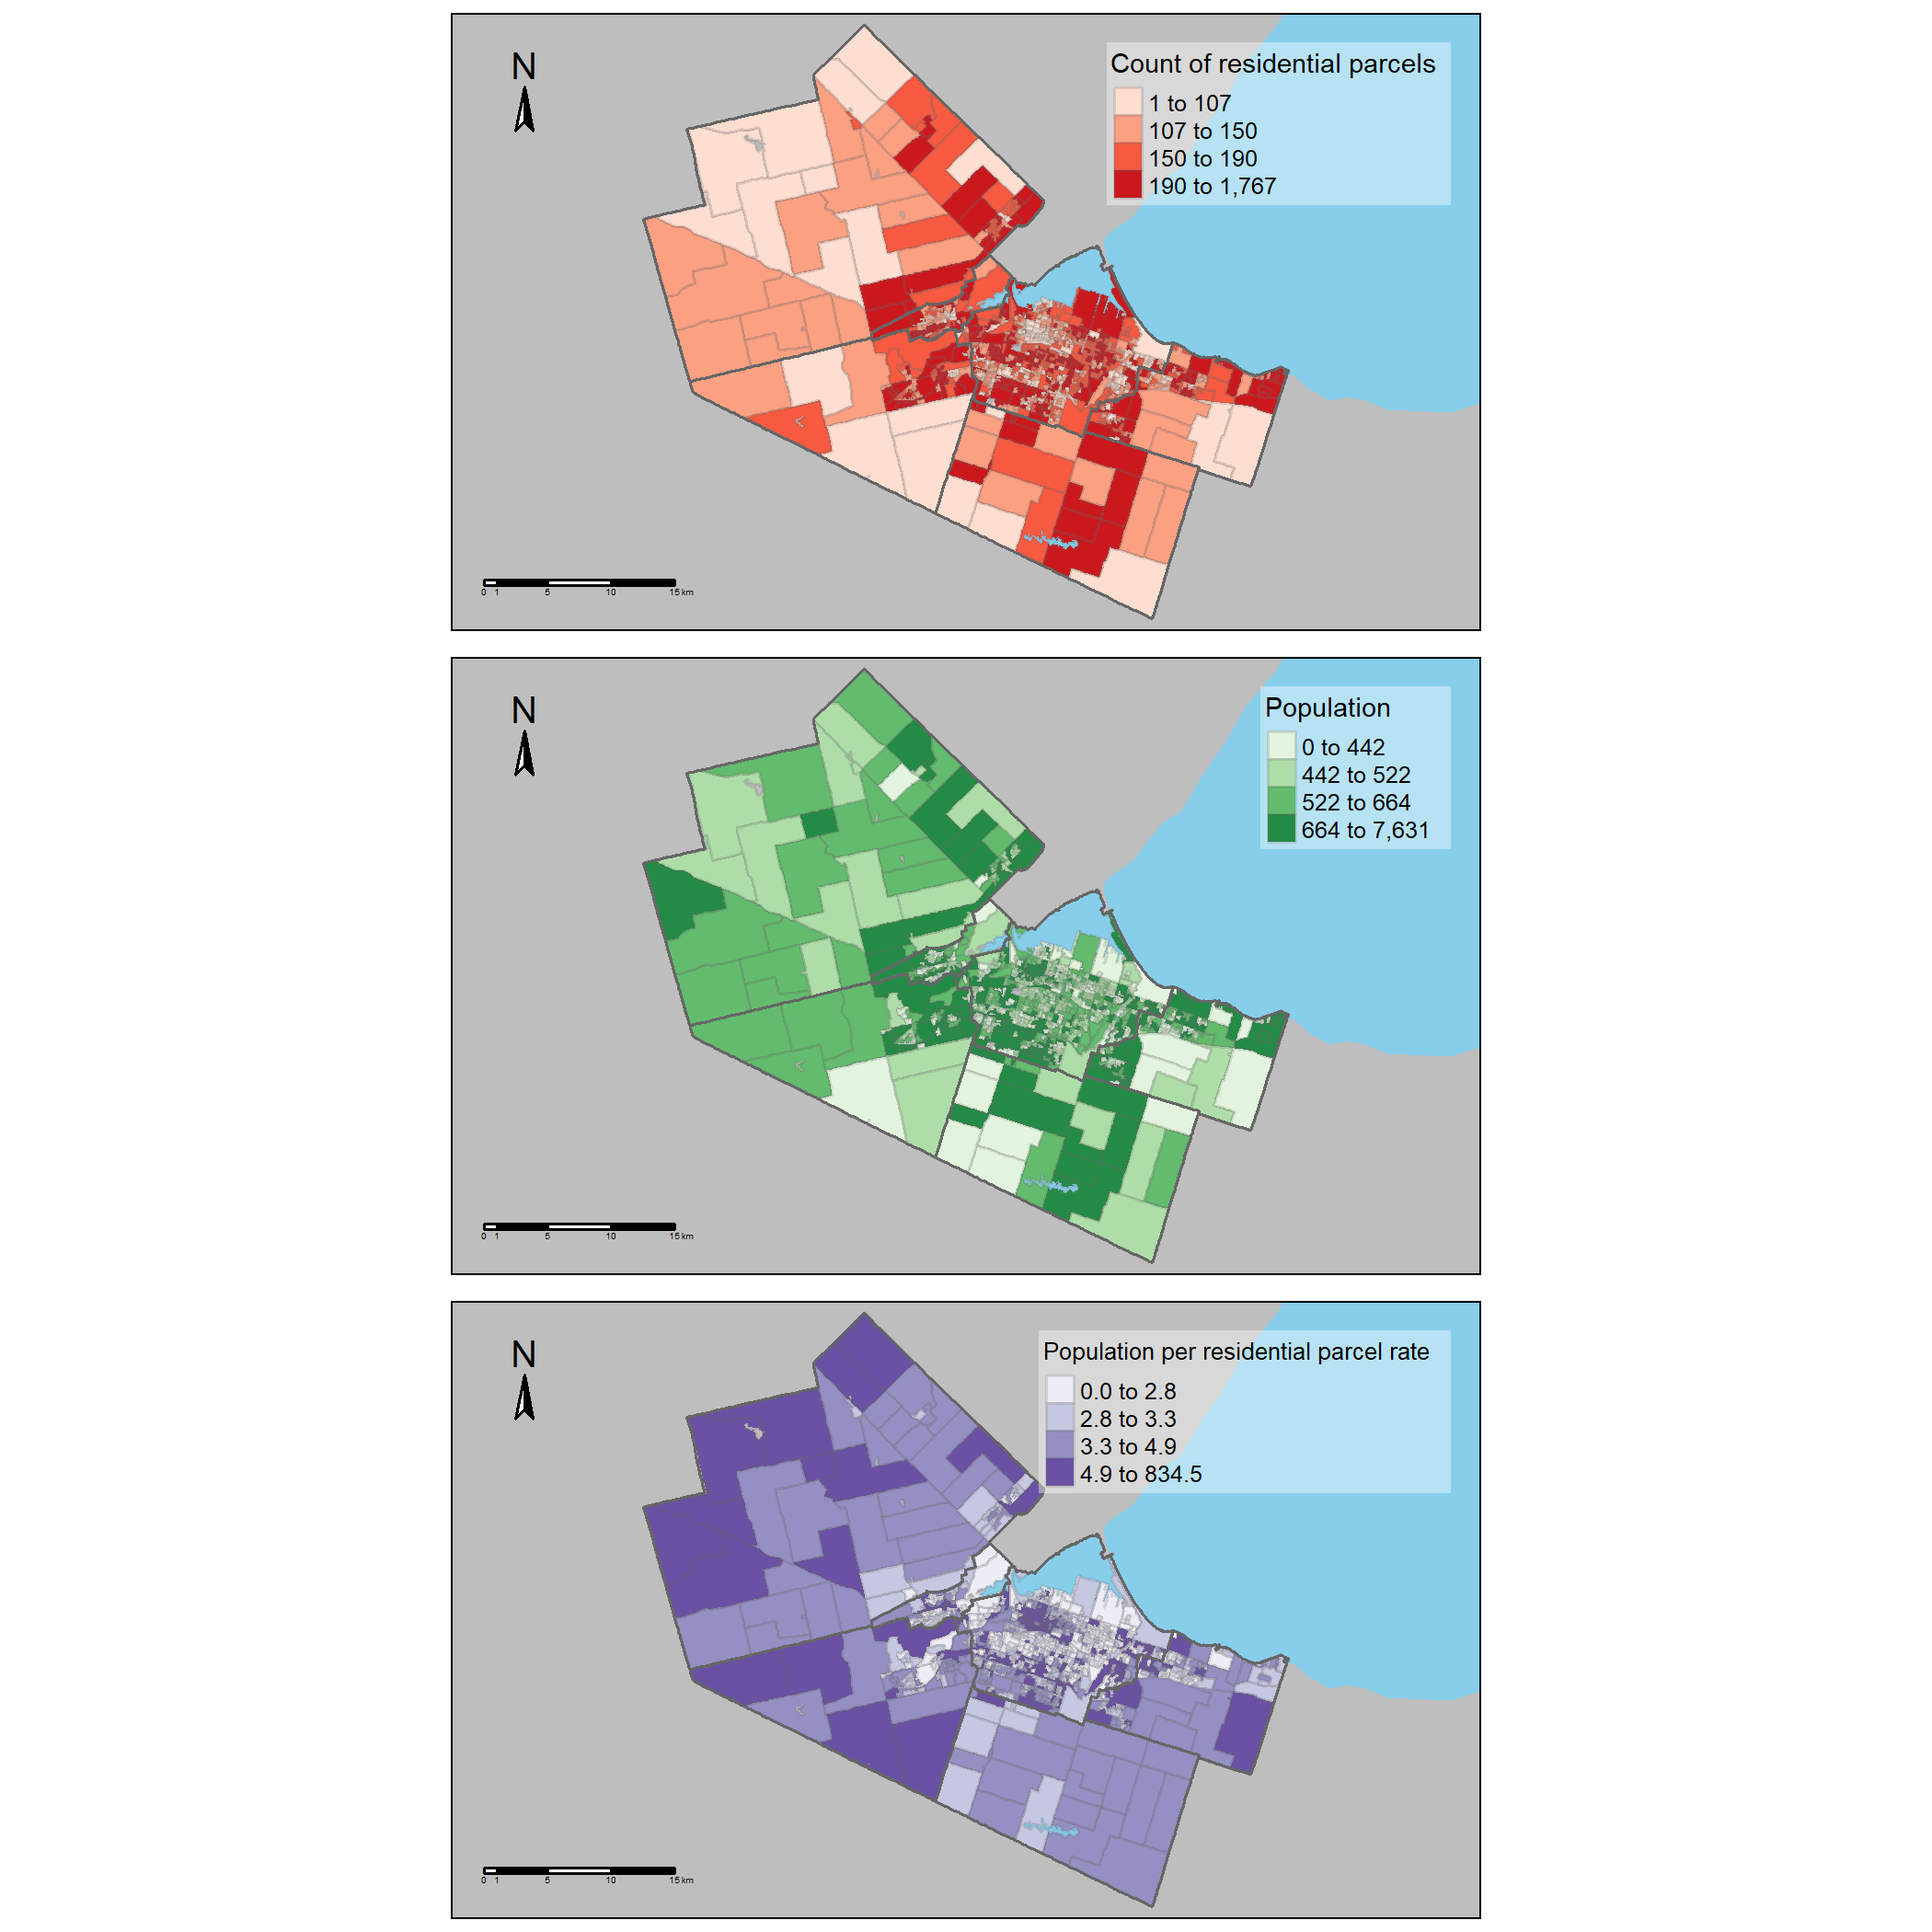
\includegraphics[width=6.25in,height=6.25in]{../figures/pop_descriptive_plots_1.png}

}

\caption{\label{fig-Fig1}The number of residential parcels per DA in
2020 (top), the population (middle) retrieved from the 2021 Canadian
Census, and the rate of population per parcel per DA (bottom). All
scales in quartiles. Basemap shapefiles are sourced from the Open Data
Hamilton Portal \citep{opendatahamiltonCityBoundary2023} and the USGS
\citep{greatlakesUSGS2010}.}

\end{figure}%

Hamilton also exhibits spatial disparities in social and economic
indicators; their spatial distribution is visualised in
Figure~\ref{fig-Fig2}. The densely populated inner city is characterised
by lower average incomes, and a higher prevalence of households living
under the low-income cutoff thresholds (LICO). Notably, the suburban
areas of the city tend to have a greater proportion of children and a
lower proportion of one parent households.

\begin{figure}

\centering{

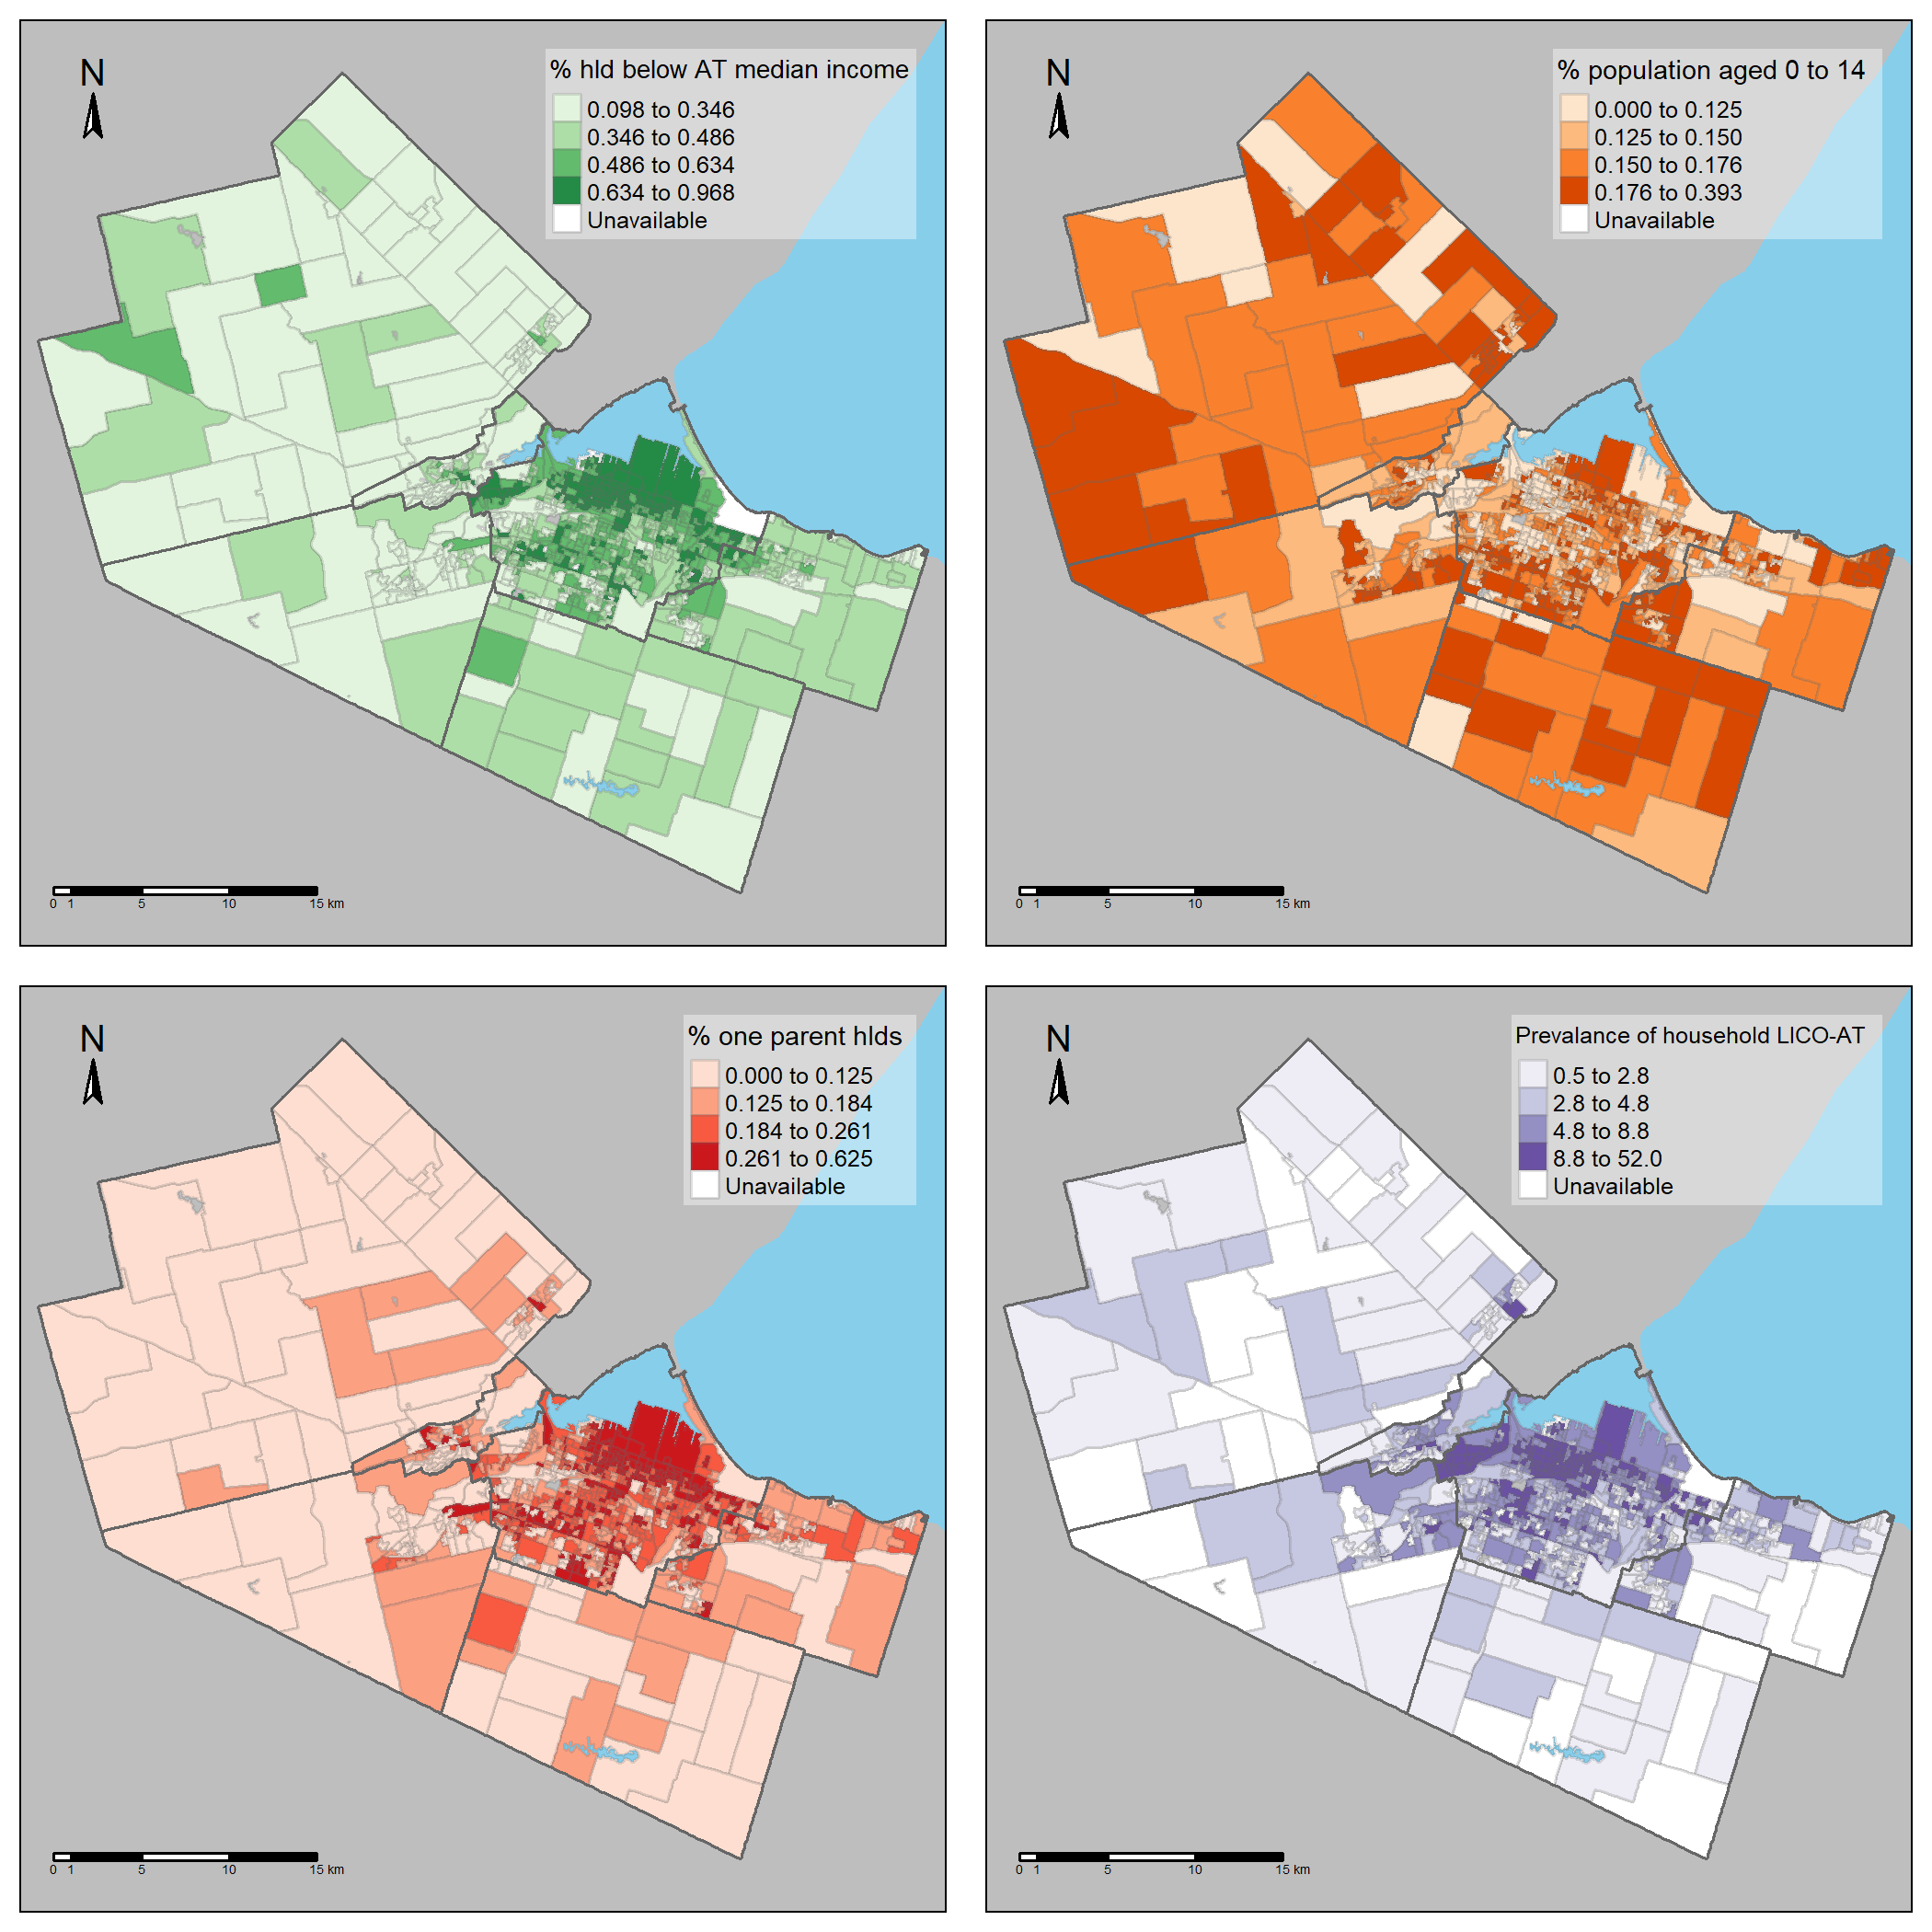
\includegraphics[width=6.25in,height=6.25in]{../figures/pop_descriptive_plots_2.png}

}

\caption{\label{fig-Fig2}Socio-economic and demographic variables that
characterise accessibility to care destinations retrieved from the 2021
Canadian Census. All scales in quartiles. Basemap shapefiles are sourced
from the Open Data Hamilton Portal
\citep{opendatahamiltonCityBoundary2023} and the USGS
\citep{greatlakesUSGS2010}.}

\end{figure}%

\newpage

\subsection{Care destination dataset}\label{care-destination-dataset}

A spatial dataset of care destinations for Hamilton was compiled as
detailed in the forthcoming work of \citet{soukhovforthcoming2024}. The
dataset includes 14 types of care destinations that were classified into
four categories: dependent-centric (e.g., the destinations for child-
and elder-centric escorting trips), grocery-centric, health-centric, and
errand-centric. Notably, these categories were generated following the
travel purpose categories created in the Mobility of Care research by
\citet{sanchezdemadariagaMeasuringMobilitiesCare2019}. Care categories,
sources of data, and descriptive notes are detailed in
Table~\ref{tbl-Tbl1}. The spatial distribution of destination type are
visualised in Figure~\ref{fig-Fig3} by their category.

\global\setlength{\Oldarrayrulewidth}{\arrayrulewidth}

\global\setlength{\Oldtabcolsep}{\tabcolsep}

\setlength{\tabcolsep}{2pt}

\renewcommand*{\arraystretch}{1}



\providecommand{\ascline}[3]{\noalign{\global\arrayrulewidth #1}\arrayrulecolor[HTML]{#2}\cline{#3}}

\begin{longtable}[c]{|p{0.67in}|p{3.94in}|p{2.09in}}

\caption{\label{tbl-Tbl1}Description of care destinations categories,
notes on data preparation and associated data sources.}

\tabularnewline

\ascline{1.5pt}{666666}{1-3}

\multicolumn{1}{>{\raggedright}m{\dimexpr 0.67in+0\tabcolsep}}{\textcolor[HTML]{000000}{\fontsize{8}{8}\selectfont{Care\ category}}} & \multicolumn{1}{>{\raggedright}m{\dimexpr 3.94in+0\tabcolsep}}{\textcolor[HTML]{000000}{\fontsize{8}{8}\selectfont{Care\ destination\ types}}} & \multicolumn{1}{>{\raggedright}m{\dimexpr 2.09in+0\tabcolsep}}{\textcolor[HTML]{000000}{\fontsize{8}{8}\selectfont{Sources}}} \\

\ascline{1.5pt}{666666}{1-3}\endfirsthead 

\ascline{1.5pt}{666666}{1-3}

\multicolumn{1}{>{\raggedright}m{\dimexpr 0.67in+0\tabcolsep}}{\textcolor[HTML]{000000}{\fontsize{8}{8}\selectfont{Care\ category}}} & \multicolumn{1}{>{\raggedright}m{\dimexpr 3.94in+0\tabcolsep}}{\textcolor[HTML]{000000}{\fontsize{8}{8}\selectfont{Care\ destination\ types}}} & \multicolumn{1}{>{\raggedright}m{\dimexpr 2.09in+0\tabcolsep}}{\textcolor[HTML]{000000}{\fontsize{8}{8}\selectfont{Sources}}} \\

\ascline{1.5pt}{666666}{1-3}\endhead



\multicolumn{1}{>{\raggedright}m{\dimexpr 0.67in+0\tabcolsep}}{\textcolor[HTML]{000000}{\fontsize{8}{0}\selectfont{Depedent-centric}}} & \multicolumn{1}{>{\raggedright}m{\dimexpr 3.94in+0\tabcolsep}}{\textcolor[HTML]{000000}{\fontsize{8}{0}\selectfont{Schools,}}\textcolor[HTML]{000000}{\fontsize{8}{0}\selectfont{\ }}\textcolor[HTML]{000000}{\fontsize{8}{0}\selectfont{daycares,}}\textcolor[HTML]{000000}{\fontsize{8}{0}\selectfont{\ }}\textcolor[HTML]{000000}{\fontsize{8}{0}\selectfont{and}}\textcolor[HTML]{000000}{\fontsize{8}{0}\selectfont{\ }}\textcolor[HTML]{000000}{\fontsize{8}{0}\selectfont{community}}\textcolor[HTML]{000000}{\fontsize{8}{0}\selectfont{\ }}\textcolor[HTML]{000000}{\fontsize{8}{0}\selectfont{centres,}}\textcolor[HTML]{000000}{\fontsize{8}{0}\selectfont{\ }}\textcolor[HTML]{000000}{\fontsize{8}{0}\selectfont{recreation}}\textcolor[HTML]{000000}{\fontsize{8}{0}\selectfont{\ }}\textcolor[HTML]{000000}{\fontsize{8}{0}\selectfont{centres,}}\textcolor[HTML]{000000}{\fontsize{8}{0}\selectfont{\ }}\textcolor[HTML]{000000}{\fontsize{8}{0}\selectfont{parks,}}\textcolor[HTML]{000000}{\fontsize{8}{0}\selectfont{\ }}\textcolor[HTML]{000000}{\fontsize{8}{0}\selectfont{senior}}\textcolor[HTML]{000000}{\fontsize{8}{0}\selectfont{\ }}\textcolor[HTML]{000000}{\fontsize{8}{0}\selectfont{centres,}}\textcolor[HTML]{000000}{\fontsize{8}{0}\selectfont{\ }}\textcolor[HTML]{000000}{\fontsize{8}{0}\selectfont{long-term}}\textcolor[HTML]{000000}{\fontsize{8}{0}\selectfont{\ }}\textcolor[HTML]{000000}{\fontsize{8}{0}\selectfont{care}}\textcolor[HTML]{000000}{\fontsize{8}{0}\selectfont{\ }}\textcolor[HTML]{000000}{\fontsize{8}{0}\selectfont{homes,}}\textcolor[HTML]{000000}{\fontsize{8}{0}\selectfont{\ }}\textcolor[HTML]{000000}{\fontsize{8}{0}\selectfont{and}}\textcolor[HTML]{000000}{\fontsize{8}{0}\selectfont{\ }}\textcolor[HTML]{000000}{\fontsize{8}{0}\selectfont{retirement}}\textcolor[HTML]{000000}{\fontsize{8}{0}\selectfont{\ }}\textcolor[HTML]{000000}{\fontsize{8}{0}\selectfont{homes:}}\textcolor[HTML]{000000}{\fontsize{8}{0}\selectfont{\ }}\textcolor[HTML]{000000}{\fontsize{8}{0}\selectfont{1,265}}\textcolor[HTML]{000000}{\fontsize{8}{0}\selectfont{\ }}\textcolor[HTML]{000000}{\fontsize{8}{0}\selectfont{locations}}\textcolor[HTML]{000000}{\fontsize{8}{0}\selectfont{\ }}\textcolor[HTML]{000000}{\fontsize{8}{0}\selectfont{are}}\textcolor[HTML]{000000}{\fontsize{8}{0}\selectfont{\ }}\textcolor[HTML]{000000}{\fontsize{8}{0}\selectfont{included.}}} & \multicolumn{1}{>{\raggedright}m{\dimexpr 2.09in+0\tabcolsep}}{\textcolor[HTML]{000000}{\fontsize{8}{0}\selectfont{(Hamilton}}\textcolor[HTML]{000000}{\fontsize{8}{0}\selectfont{\ }}\textcolor[HTML]{000000}{\fontsize{8}{0}\selectfont{2022a,}}\textcolor[HTML]{000000}{\fontsize{8}{0}\selectfont{\ }}\textcolor[HTML]{000000}{\fontsize{8}{0}\selectfont{2023,}}\textcolor[HTML]{000000}{\fontsize{8}{0}\selectfont{\ }}\textcolor[HTML]{000000}{\fontsize{8}{0}\selectfont{2022c,}}\textcolor[HTML]{000000}{\fontsize{8}{0}\selectfont{\ }}\textcolor[HTML]{000000}{\fontsize{8}{0}\selectfont{2022d;}}\textcolor[HTML]{000000}{\fontsize{8}{0}\selectfont{\ }}\textcolor[HTML]{000000}{\fontsize{8}{0}\selectfont{Ontario}}\textcolor[HTML]{000000}{\fontsize{8}{0}\selectfont{\ }}\textcolor[HTML]{000000}{\fontsize{8}{0}\selectfont{2023;}}\textcolor[HTML]{000000}{\fontsize{8}{0}\selectfont{\ }}\textcolor[HTML]{000000}{\fontsize{8}{0}\selectfont{Ontario GeoHub}}\textcolor[HTML]{000000}{\fontsize{8}{0}\selectfont{\ }}\textcolor[HTML]{000000}{\fontsize{8}{0}\selectfont{2023)}}} \\





\multicolumn{1}{>{\raggedright}m{\dimexpr 0.67in+0\tabcolsep}}{\textcolor[HTML]{000000}{\fontsize{8}{0}\selectfont{Grocery-centric}}} & \multicolumn{1}{>{\raggedright}m{\dimexpr 3.94in+0\tabcolsep}}{\textcolor[HTML]{000000}{\fontsize{8}{0}\selectfont{Convenience}}\textcolor[HTML]{000000}{\fontsize{8}{0}\selectfont{\ }}\textcolor[HTML]{000000}{\fontsize{8}{0}\selectfont{stores}}\textcolor[HTML]{000000}{\fontsize{8}{0}\selectfont{\ }}\textcolor[HTML]{000000}{\fontsize{8}{0}\selectfont{and}}\textcolor[HTML]{000000}{\fontsize{8}{0}\selectfont{\ }}\textcolor[HTML]{000000}{\fontsize{8}{0}\selectfont{grocery}}\textcolor[HTML]{000000}{\fontsize{8}{0}\selectfont{\ }}\textcolor[HTML]{000000}{\fontsize{8}{0}\selectfont{stores}}\textcolor[HTML]{000000}{\fontsize{8}{0}\selectfont{\ }}\textcolor[HTML]{000000}{\fontsize{8}{0}\selectfont{(e.g.,}}\textcolor[HTML]{000000}{\fontsize{8}{0}\selectfont{\ }}\textcolor[HTML]{000000}{\fontsize{8}{0}\selectfont{large}}\textcolor[HTML]{000000}{\fontsize{8}{0}\selectfont{\ }}\textcolor[HTML]{000000}{\fontsize{8}{0}\selectfont{retailers}}\textcolor[HTML]{000000}{\fontsize{8}{0}\selectfont{\ }}\textcolor[HTML]{000000}{\fontsize{8}{0}\selectfont{as}}\textcolor[HTML]{000000}{\fontsize{8}{0}\selectfont{\ }}\textcolor[HTML]{000000}{\fontsize{8}{0}\selectfont{well}}\textcolor[HTML]{000000}{\fontsize{8}{0}\selectfont{\ }}\textcolor[HTML]{000000}{\fontsize{8}{0}\selectfont{as}}\textcolor[HTML]{000000}{\fontsize{8}{0}\selectfont{\ }}\textcolor[HTML]{000000}{\fontsize{8}{0}\selectfont{speciality}}\textcolor[HTML]{000000}{\fontsize{8}{0}\selectfont{\ }}\textcolor[HTML]{000000}{\fontsize{8}{0}\selectfont{food}}\textcolor[HTML]{000000}{\fontsize{8}{0}\selectfont{\ }}\textcolor[HTML]{000000}{\fontsize{8}{0}\selectfont{grocers,}}\textcolor[HTML]{000000}{\fontsize{8}{0}\selectfont{\ }}\textcolor[HTML]{000000}{\fontsize{8}{0}\selectfont{health}}\textcolor[HTML]{000000}{\fontsize{8}{0}\selectfont{\ }}\textcolor[HTML]{000000}{\fontsize{8}{0}\selectfont{food}}\textcolor[HTML]{000000}{\fontsize{8}{0}\selectfont{\ }}\textcolor[HTML]{000000}{\fontsize{8}{0}\selectfont{grocers):}}\textcolor[HTML]{000000}{\fontsize{8}{0}\selectfont{\ }}\textcolor[HTML]{000000}{\fontsize{8}{0}\selectfont{381}}\textcolor[HTML]{000000}{\fontsize{8}{0}\selectfont{\ }}\textcolor[HTML]{000000}{\fontsize{8}{0}\selectfont{destinations}}\textcolor[HTML]{000000}{\fontsize{8}{0}\selectfont{\ }}\textcolor[HTML]{000000}{\fontsize{8}{0}\selectfont{are}}\textcolor[HTML]{000000}{\fontsize{8}{0}\selectfont{\ }}\textcolor[HTML]{000000}{\fontsize{8}{0}\selectfont{included.}}} & \multicolumn{1}{>{\raggedright}m{\dimexpr 2.09in+0\tabcolsep}}{\textcolor[HTML]{000000}{\fontsize{8}{0}\selectfont{(Axle Data}}\textcolor[HTML]{000000}{\fontsize{8}{0}\selectfont{\ }}\textcolor[HTML]{000000}{\fontsize{8}{0}\selectfont{2023)}}} \\





\multicolumn{1}{>{\raggedright}m{\dimexpr 0.67in+0\tabcolsep}}{\textcolor[HTML]{000000}{\fontsize{8}{0}\selectfont{Health-centric}}} & \multicolumn{1}{>{\raggedright}m{\dimexpr 3.94in+0\tabcolsep}}{\textcolor[HTML]{000000}{\fontsize{8}{0}\selectfont{Hospitals,}}\textcolor[HTML]{000000}{\fontsize{8}{0}\selectfont{\ }}\textcolor[HTML]{000000}{\fontsize{8}{0}\selectfont{pharmacies,}}\textcolor[HTML]{000000}{\fontsize{8}{0}\selectfont{\ }}\textcolor[HTML]{000000}{\fontsize{8}{0}\selectfont{clinics,}}\textcolor[HTML]{000000}{\fontsize{8}{0}\selectfont{\ }}\textcolor[HTML]{000000}{\fontsize{8}{0}\selectfont{and}}\textcolor[HTML]{000000}{\fontsize{8}{0}\selectfont{\ }}\textcolor[HTML]{000000}{\fontsize{8}{0}\selectfont{dentist}}\textcolor[HTML]{000000}{\fontsize{8}{0}\selectfont{\ }}\textcolor[HTML]{000000}{\fontsize{8}{0}\selectfont{offices:}}\textcolor[HTML]{000000}{\fontsize{8}{0}\selectfont{\ }}\textcolor[HTML]{000000}{\fontsize{8}{0}\selectfont{421}}\textcolor[HTML]{000000}{\fontsize{8}{0}\selectfont{\ }}\textcolor[HTML]{000000}{\fontsize{8}{0}\selectfont{destinations}}\textcolor[HTML]{000000}{\fontsize{8}{0}\selectfont{\ }}\textcolor[HTML]{000000}{\fontsize{8}{0}\selectfont{are}}\textcolor[HTML]{000000}{\fontsize{8}{0}\selectfont{\ }}\textcolor[HTML]{000000}{\fontsize{8}{0}\selectfont{identified.}}} & \multicolumn{1}{>{\raggedright}m{\dimexpr 2.09in+0\tabcolsep}}{\textcolor[HTML]{000000}{\fontsize{8}{0}\selectfont{(Ontario GeoHub}}\textcolor[HTML]{000000}{\fontsize{8}{0}\selectfont{\ }}\textcolor[HTML]{000000}{\fontsize{8}{0}\selectfont{2023;}}\textcolor[HTML]{000000}{\fontsize{8}{0}\selectfont{\ }}\textcolor[HTML]{000000}{\fontsize{8}{0}\selectfont{HNHB Healthline}}\textcolor[HTML]{000000}{\fontsize{8}{0}\selectfont{\ }}\textcolor[HTML]{000000}{\fontsize{8}{0}\selectfont{2023)}}} \\





\multicolumn{1}{>{\raggedright}m{\dimexpr 0.67in+0\tabcolsep}}{\textcolor[HTML]{000000}{\fontsize{8}{0}\selectfont{Errand-centric}}} & \multicolumn{1}{>{\raggedright}m{\dimexpr 3.94in+0\tabcolsep}}{\textcolor[HTML]{000000}{\fontsize{8}{0}\selectfont{Libraries,}}\textcolor[HTML]{000000}{\fontsize{8}{0}\selectfont{\ }}\textcolor[HTML]{000000}{\fontsize{8}{0}\selectfont{post}}\textcolor[HTML]{000000}{\fontsize{8}{0}\selectfont{\ }}\textcolor[HTML]{000000}{\fontsize{8}{0}\selectfont{offices,}}\textcolor[HTML]{000000}{\fontsize{8}{0}\selectfont{\ }}\textcolor[HTML]{000000}{\fontsize{8}{0}\selectfont{and}}\textcolor[HTML]{000000}{\fontsize{8}{0}\selectfont{\ }}\textcolor[HTML]{000000}{\fontsize{8}{0}\selectfont{banks:}}\textcolor[HTML]{000000}{\fontsize{8}{0}\selectfont{\ }}\textcolor[HTML]{000000}{\fontsize{8}{0}\selectfont{158}}\textcolor[HTML]{000000}{\fontsize{8}{0}\selectfont{\ }}\textcolor[HTML]{000000}{\fontsize{8}{0}\selectfont{destinations}}\textcolor[HTML]{000000}{\fontsize{8}{0}\selectfont{\ }}\textcolor[HTML]{000000}{\fontsize{8}{0}\selectfont{are}}\textcolor[HTML]{000000}{\fontsize{8}{0}\selectfont{\ }}\textcolor[HTML]{000000}{\fontsize{8}{0}\selectfont{identified.}}} & \multicolumn{1}{>{\raggedright}m{\dimexpr 2.09in+0\tabcolsep}}{\textcolor[HTML]{000000}{\fontsize{8}{0}\selectfont{(Hamilton}}\textcolor[HTML]{000000}{\fontsize{8}{0}\selectfont{\ }}\textcolor[HTML]{000000}{\fontsize{8}{0}\selectfont{2022b;}}\textcolor[HTML]{000000}{\fontsize{8}{0}\selectfont{\ }}\textcolor[HTML]{000000}{\fontsize{8}{0}\selectfont{Axle Data}}\textcolor[HTML]{000000}{\fontsize{8}{0}\selectfont{\ }}\textcolor[HTML]{000000}{\fontsize{8}{0}\selectfont{2023;}}\textcolor[HTML]{000000}{\fontsize{8}{0}\selectfont{\ }}\textcolor[HTML]{000000}{\fontsize{8}{0}\selectfont{Canada Post}}\textcolor[HTML]{000000}{\fontsize{8}{0}\selectfont{\ }}\textcolor[HTML]{000000}{\fontsize{8}{0}\selectfont{2023;}}\textcolor[HTML]{000000}{\fontsize{8}{0}\selectfont{\ }}\textcolor[HTML]{000000}{\fontsize{8}{0}\selectfont{BMO}}\textcolor[HTML]{000000}{\fontsize{8}{0}\selectfont{\ }}\textcolor[HTML]{000000}{\fontsize{8}{0}\selectfont{2023;}}\textcolor[HTML]{000000}{\fontsize{8}{0}\selectfont{\ }}\textcolor[HTML]{000000}{\fontsize{8}{0}\selectfont{HSBC}}\textcolor[HTML]{000000}{\fontsize{8}{0}\selectfont{\ }}\textcolor[HTML]{000000}{\fontsize{8}{0}\selectfont{2023;}}\textcolor[HTML]{000000}{\fontsize{8}{0}\selectfont{\ }}\textcolor[HTML]{000000}{\fontsize{8}{0}\selectfont{National Bank}}\textcolor[HTML]{000000}{\fontsize{8}{0}\selectfont{\ }}\textcolor[HTML]{000000}{\fontsize{8}{0}\selectfont{2023;}}\textcolor[HTML]{000000}{\fontsize{8}{0}\selectfont{\ }}\textcolor[HTML]{000000}{\fontsize{8}{0}\selectfont{RBC}}\textcolor[HTML]{000000}{\fontsize{8}{0}\selectfont{\ }}\textcolor[HTML]{000000}{\fontsize{8}{0}\selectfont{2023;}}\textcolor[HTML]{000000}{\fontsize{8}{0}\selectfont{\ }}\textcolor[HTML]{000000}{\fontsize{8}{0}\selectfont{Scotiabank}}\textcolor[HTML]{000000}{\fontsize{8}{0}\selectfont{\ }}\textcolor[HTML]{000000}{\fontsize{8}{0}\selectfont{2023;}}\textcolor[HTML]{000000}{\fontsize{8}{0}\selectfont{\ }}\textcolor[HTML]{000000}{\fontsize{8}{0}\selectfont{TD Bank}}\textcolor[HTML]{000000}{\fontsize{8}{0}\selectfont{\ }}\textcolor[HTML]{000000}{\fontsize{8}{0}\selectfont{2023)}}\textcolor[HTML]{000000}{\fontsize{8}{0}\selectfont{.}}} \\

\ascline{1.5pt}{666666}{1-3}


\end{longtable}

\arrayrulecolor[HTML]{000000}

\global\setlength{\arrayrulewidth}{\Oldarrayrulewidth}

\global\setlength{\tabcolsep}{\Oldtabcolsep}

\renewcommand*{\arraystretch}{1}

\begin{figure}

\centering{

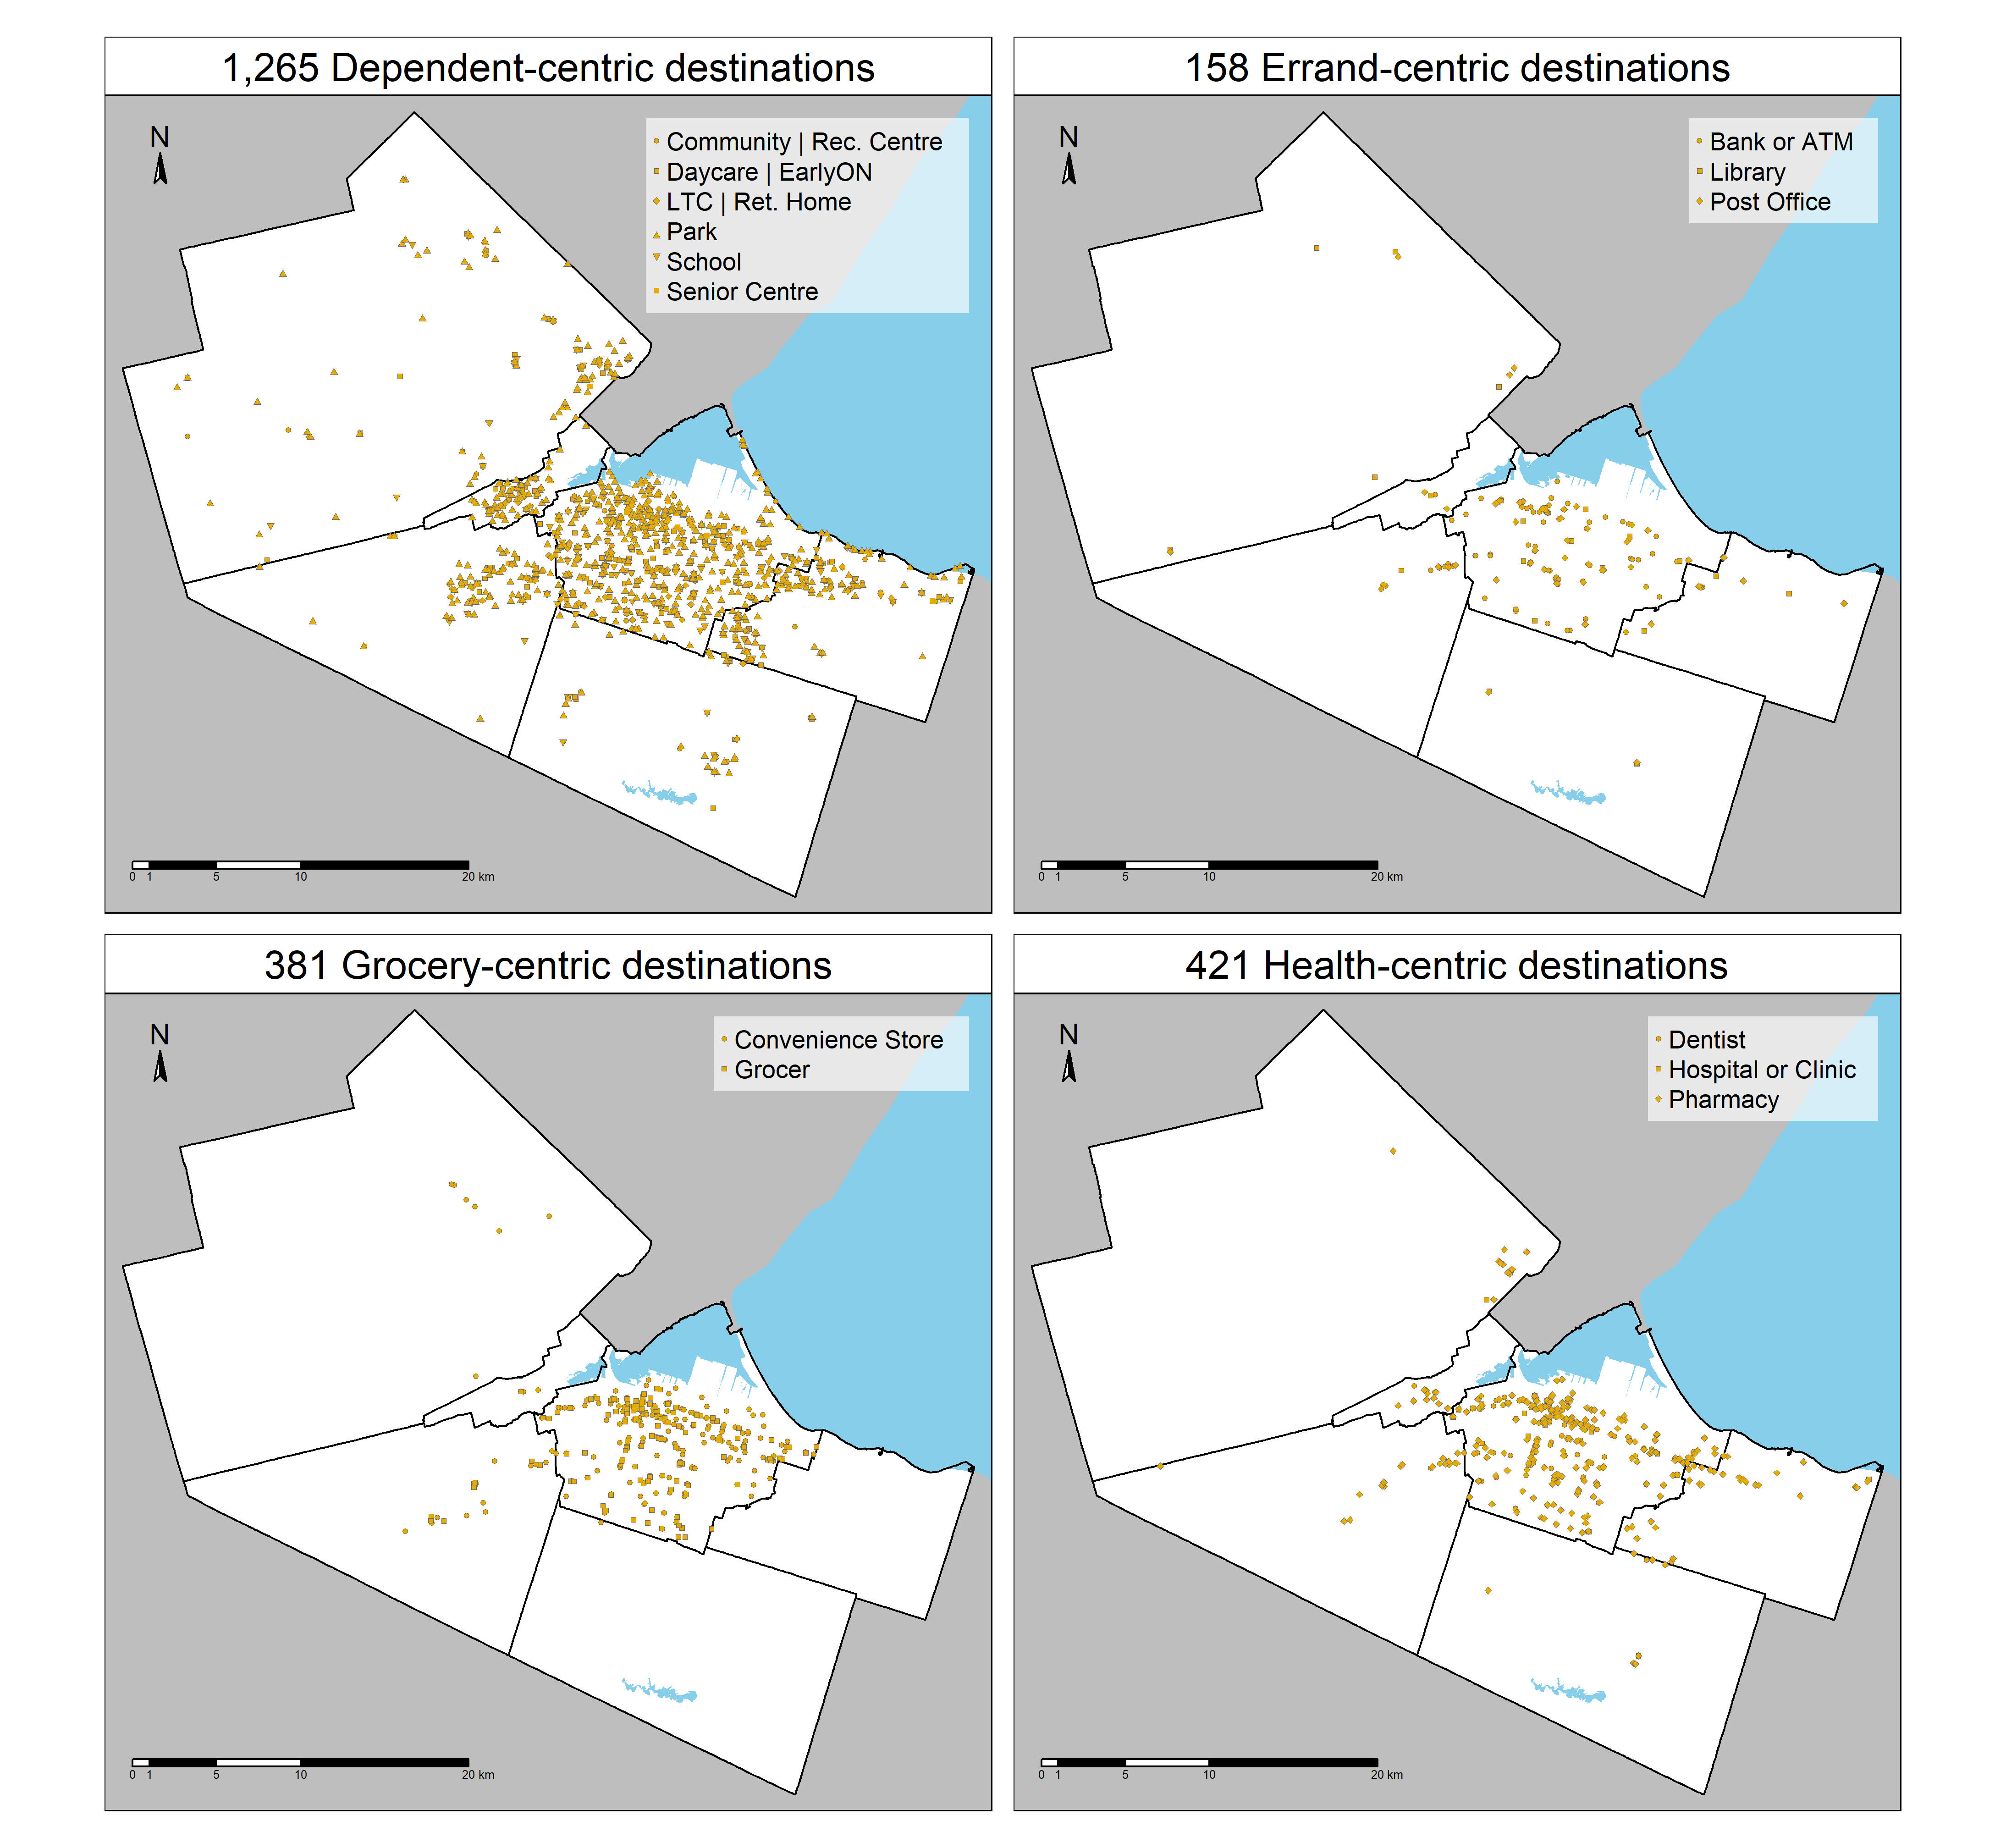
\includegraphics[width=6.25in,height=6.25in]{../figures/care_categories_plot.png}

}

\caption{\label{fig-Fig3}The locations of care destinations in Hamilton
separated by the author-generated categories of: dependent-, errand-,
grocery- and health- centric care categories. Basemap shapefiles are
sourced from the Open Data Hamilton Portal
\citep{opendatahamiltonCityBoundary2023} and the USGS
\citep{greatlakesUSGS2010}.}

\end{figure}%

\newpage

\subsection{Travel time to care destinations
estimations}\label{travel-time-to-care-destinations-estimations}

Travel behaviour to care-oriented destinations is often uncounted and
hence comprehensive travel times to all destination types in
Table~\ref{tbl-Tbl1} is unavailable. To overcome this gap, travel time
from residential parcel locations in Hamilton and care destinations in
Figure~\ref{fig-Fig3} are approximated assuming travel by foot at an
average speed (3.6 km/hr). This estimation is done using the
`travel\_time\_matrix()' function from the \{r5r\} package
\citep{pereiraR5rRapidRealistic2021} using R version 4.3.2
\citep{coreR2023}. The inputs into the function are: the locations of
143,882 residential parcels as origins, the 2,225 care locations as
destinations, and a OpenStreetMap road network including walking
infrastructure \citep{geofabrikOntarioCanadaOpen2023}. In line with the
15-Minute City, a maximum walking travel time of 15 minutes is specified
and an origin-destination travel time matrix of the shortest travel time
from origin to destination is calculated. The resulting matrix contains
2,014,502 rows, representing walking travel times from each parcel to
reachable care destinations within 15 minutes.

\section{Methods}\label{methods}

The following sub-sections detail the methods to classify Hamilton into
spatial degrees of \emph{caring 15-minute neighbourhood}. First,
accessibility to each of the 14 destination types from each of the
143,882 residential parcel locations is described. Second, the entropy
measures used to calculate the diversity of accessibility to each of the
care categories is detailed. Third, we describe how accessibility and
diversity values for each parcel are input into a Self-Organizing Map
(SOM) algorithm, and how the resulting clusters are analyzed using a
Decision Tree algorithm to narrate residential profiles based on
socio-economic variables. In sum, this methodology presents a
data-driven approach to examine what neighbourhoods in a city have the
potential to provide 15-minute caring access, at what level of intensity
and completeness, and the socio-economic characteristics of those who
are most benefited or burdened.

\subsection{Accessibility: the cumulative opportunity
measure}\label{accessibility-the-cumulative-opportunity-measure}

To capture the quantity of access to each type of destinations, a
cumulative opportunity accessibility score \(S^t_i\) is calculated.
Scores for each of the 14 care destination types \(t\) is calculated for
every parcel \(i\). The calculation takes the following mathematical
form:

\[
S^t_i=\sum_{j}O_j^{t}\cdot f(c_{ij})
\] \noindent Where:

\begin{itemize}
\tightlist
\item
  \(i\) is a set of parcel point origin locations.
\item
  \(j\) is a set of care destination locations of type \(t\).
\item
  \(O^t_j\) is a number of opportunities of category type \(t\) at
  \(j\).
\item
  \(c_{ij}\) is the travel cost between \(i\) and \(j\).
\item
  \(f(\cdot)\) is an impedance function of \(c_{ij}\); within the
  cumulative opportunity approach, it is a binary function that takes
  the value of 1 if \(c_{ij}\) is less than a selected value
  \citep{handyMeasuringAccessibilityExploration1997}.
\item
  \(S_{i}^t\) is the cumulative opportunity accessibility score, the sum
  of weighted opportunities reachable within \(f(\cdot)\), at each \(i\)
  for each \(t\).
\end{itemize}

\subsection{Diversity in opportunity accessibility: the entropy
measure}\label{diversity-in-opportunity-accessibility-the-entropy-measure}

The entropy measure, as defined in \citet{cerveroTravelDemand3Ds1997},
is used to represent the diversity of care destination accessibility.
For each parcel, a value between 0 to 1 is calculated, where 1
represents total evenness in the number of care opportunities in each
category that can be reached. The mathematical formulation takes the
following form:

\[
D_{i} = \frac{-\sum_{t} [S_i^{t} / \sum_{t}S^{t}_{i} \times ln(S_i^{t} / \sum_{t}S^{t}_{i} )]}{ln(n_t)}
\]

\noindent Where:

\begin{itemize}
\tightlist
\item
  \(i\) is a set of parcel point origin locations.
\item
  \(t\) is a set of care destination types (e.g., school, grocery, park,
  etc.)
\item
  \(n_t\) is the count of care destination types \(t\). In this work,
  this value is 14.
\item
  \(S_{i}^t\) is the cumulative opportunity accessibility score, the sum
  of weighted opportunities reachable within a 15-minute walk from
  \(i\).
\item
  \(D_i\) is the diversity score.
\end{itemize}

Notably, \(D_i\) represents evenness in the type of care categories a
parcel can access. For example, if a parcel has an access score of
\(S_i^t = 0.5\) for all destination types, it will receive a diversity
score of \(D_i = 1\), just as if it had an access score of
\(S_i^t = 10\) for each destination. Conversely, a parcel may be
assigned a low \(D_i\) score if its accessibility scores differ across
categories, regardless of whether those scores are low or high.

\subsection{Machine learning classification: SOM and Decision
Trees}\label{machine-learning-classification-som-and-decision-trees}

We use two machine learning techniques in this work. First, SOM is an
unsupervised technique implemented to reduce the data dimensionality and
create interpretable clusters related to the intensity and completeness
of caring access. This is done by imputing each parcel as an observation
with its associated accessibility and diversity attributes, and the data
being rearranged onto a two-dimensional space based on its minimizing
dissimilarity in its neighbourhood. An appropriate number of
superclusters are selected and assigned labels based on the quantity and
diversity of care access provided, i.e., the degree by each the parcel
is located in a \emph{caring 15-minute neighbourhood}. Then, a Decision
Tree is run to characterise the socio-economic profiles of who resides
in neighbourhoods associated with the superclusters. Together, this
combined approach leverages the unsupervised data-driven classification
power of the SOM with the interpretation of Decision Trees. The
procedure used in this work is similar to that used in
\citet{victorianoTimeSpaceMoney2020}. In this work, rather than each
observation representing an individual's daily mobility behaviour (with
associated variables), each observation represents a parcel location
with calculated care accessibility and accessibility diversity scores.

For the SOM step, the function `trainSOM()' from \{SOMbrero\} R package
is used \citep{VillaVialaneix2017}. The input variables include the
143,882 parcels, each as individual observation along with 15 variables:
the 14 calculated accessibility scores \(S_i^t\), normalized to the
min-max range score within each \(t\), and one diversity value \(D_i\).
Otherwise, defaults for all other parameters are assumed, relying on the
data-driven heuristics embedded in the `trainSOM()' function.
Consequently, a 100 node (10 by 10 grid) SOM structure using euclidean
distance and square topology is produced. Simply put, the SOM algorithm
proceeds as follows: a 2D grid of nodes is created as specified by the
analyst, where a node represents a point in the reduced-dimensional
space. Upon initialization, each node is assigned a random weight vector
of the same dimension as the input data (in our case, 15). From the
input data, a random observation with its associated weight vector
(i.e., one parcel point with 15 variables) is selected and the Euclidean
distance between its weight vector and all nodes in the grid are
calculated. The node with the smallest distance (i.e., the smallest
dissimilarity) is labelled the `best matching unit' as it is the node
that best represents the input observation. After this best matching
unit is identified, its own weight and its neighbouring nodes are
updated to become more like the input observation. The process of
finding best matching units and updating their weights is repeated for
every observation, multiple times, until the results converge. As
mentioned, this competitive learning process produces a 100 node SOM
structure where each observation (parcel) is assigned to 1 node with an
associated dissimilarity index. The SOM output is typically examined
through a dissimilarity dendogram and an associated dissimilarity
variance explained plot to select an appropriately representative
`superclusters'
\citep{VillaVialaneix2017, victorianoTimeSpaceMoney2020}.

For the Decision Tree step, the supercluster-classified parcels
identified in the SOM step are used as \emph{labels} and socio-economic
and demographic indicators related to the Mobility of Care literature
are used as \emph{features}. Features are retrieved from the 2021
Canadian Census \citep{governmentofcanadaCensusPopulation2023}. This
step creates residential profiles of the superclusters, allowing us to
explore the characteristics of residents within the superclusters in a
data-driven way. To estimate the Decision Tree, the `rpart()' function
in the \{rpart\} R package is used \citep{Therneau2023}; default
parameters for classification splitting along with each value being
weighted by the population present in the associated DA is assumed. The
Decision Tree algorithm is a supervised learning technique that begins
by splitting a subset of the input data into branches based on a
selected feature with the lowest impurity score (i.e., the least mixing
of label membership within a branch). This process is recursively
repeated for each data subset, selecting the next best feature.
Ultimately, the data is classified into distinct classes, with class
membership explained by traversing the branches defined by the features
that characterise the partitions within the Decision Tree. Notably, the
absence of features from the Decision Tree does not necessarily imply
they are irrelevant for classification, rather, they are less relevant
than other features. Put another way, when considering features that are
highly correlated, such as income level and LICO, not all relevant
variables may be present in the tree
\citep{victorianoTimeSpaceMoney2020}.

\section{Results}\label{results}

\subsection{Overview of access to care
destinations}\label{overview-of-access-to-care-destinations}

How many care destinations can be reached within a 15-minute walk is
summed for each of the four care categories defined in
Table~\ref{tbl-Tbl1}. The median parcel value for each DA is visualised
in Figure~\ref{fig-Fig4} and the median parcel diversity of care
destinations accessible is presented in Figure~\ref{fig-Fig5}. Together,
Figure~\ref{fig-Fig4} and Figure~\ref{fig-Fig5} represent summaries of
15 variables that served as inputs into the SOM algorithm.

\begin{figure}

\centering{

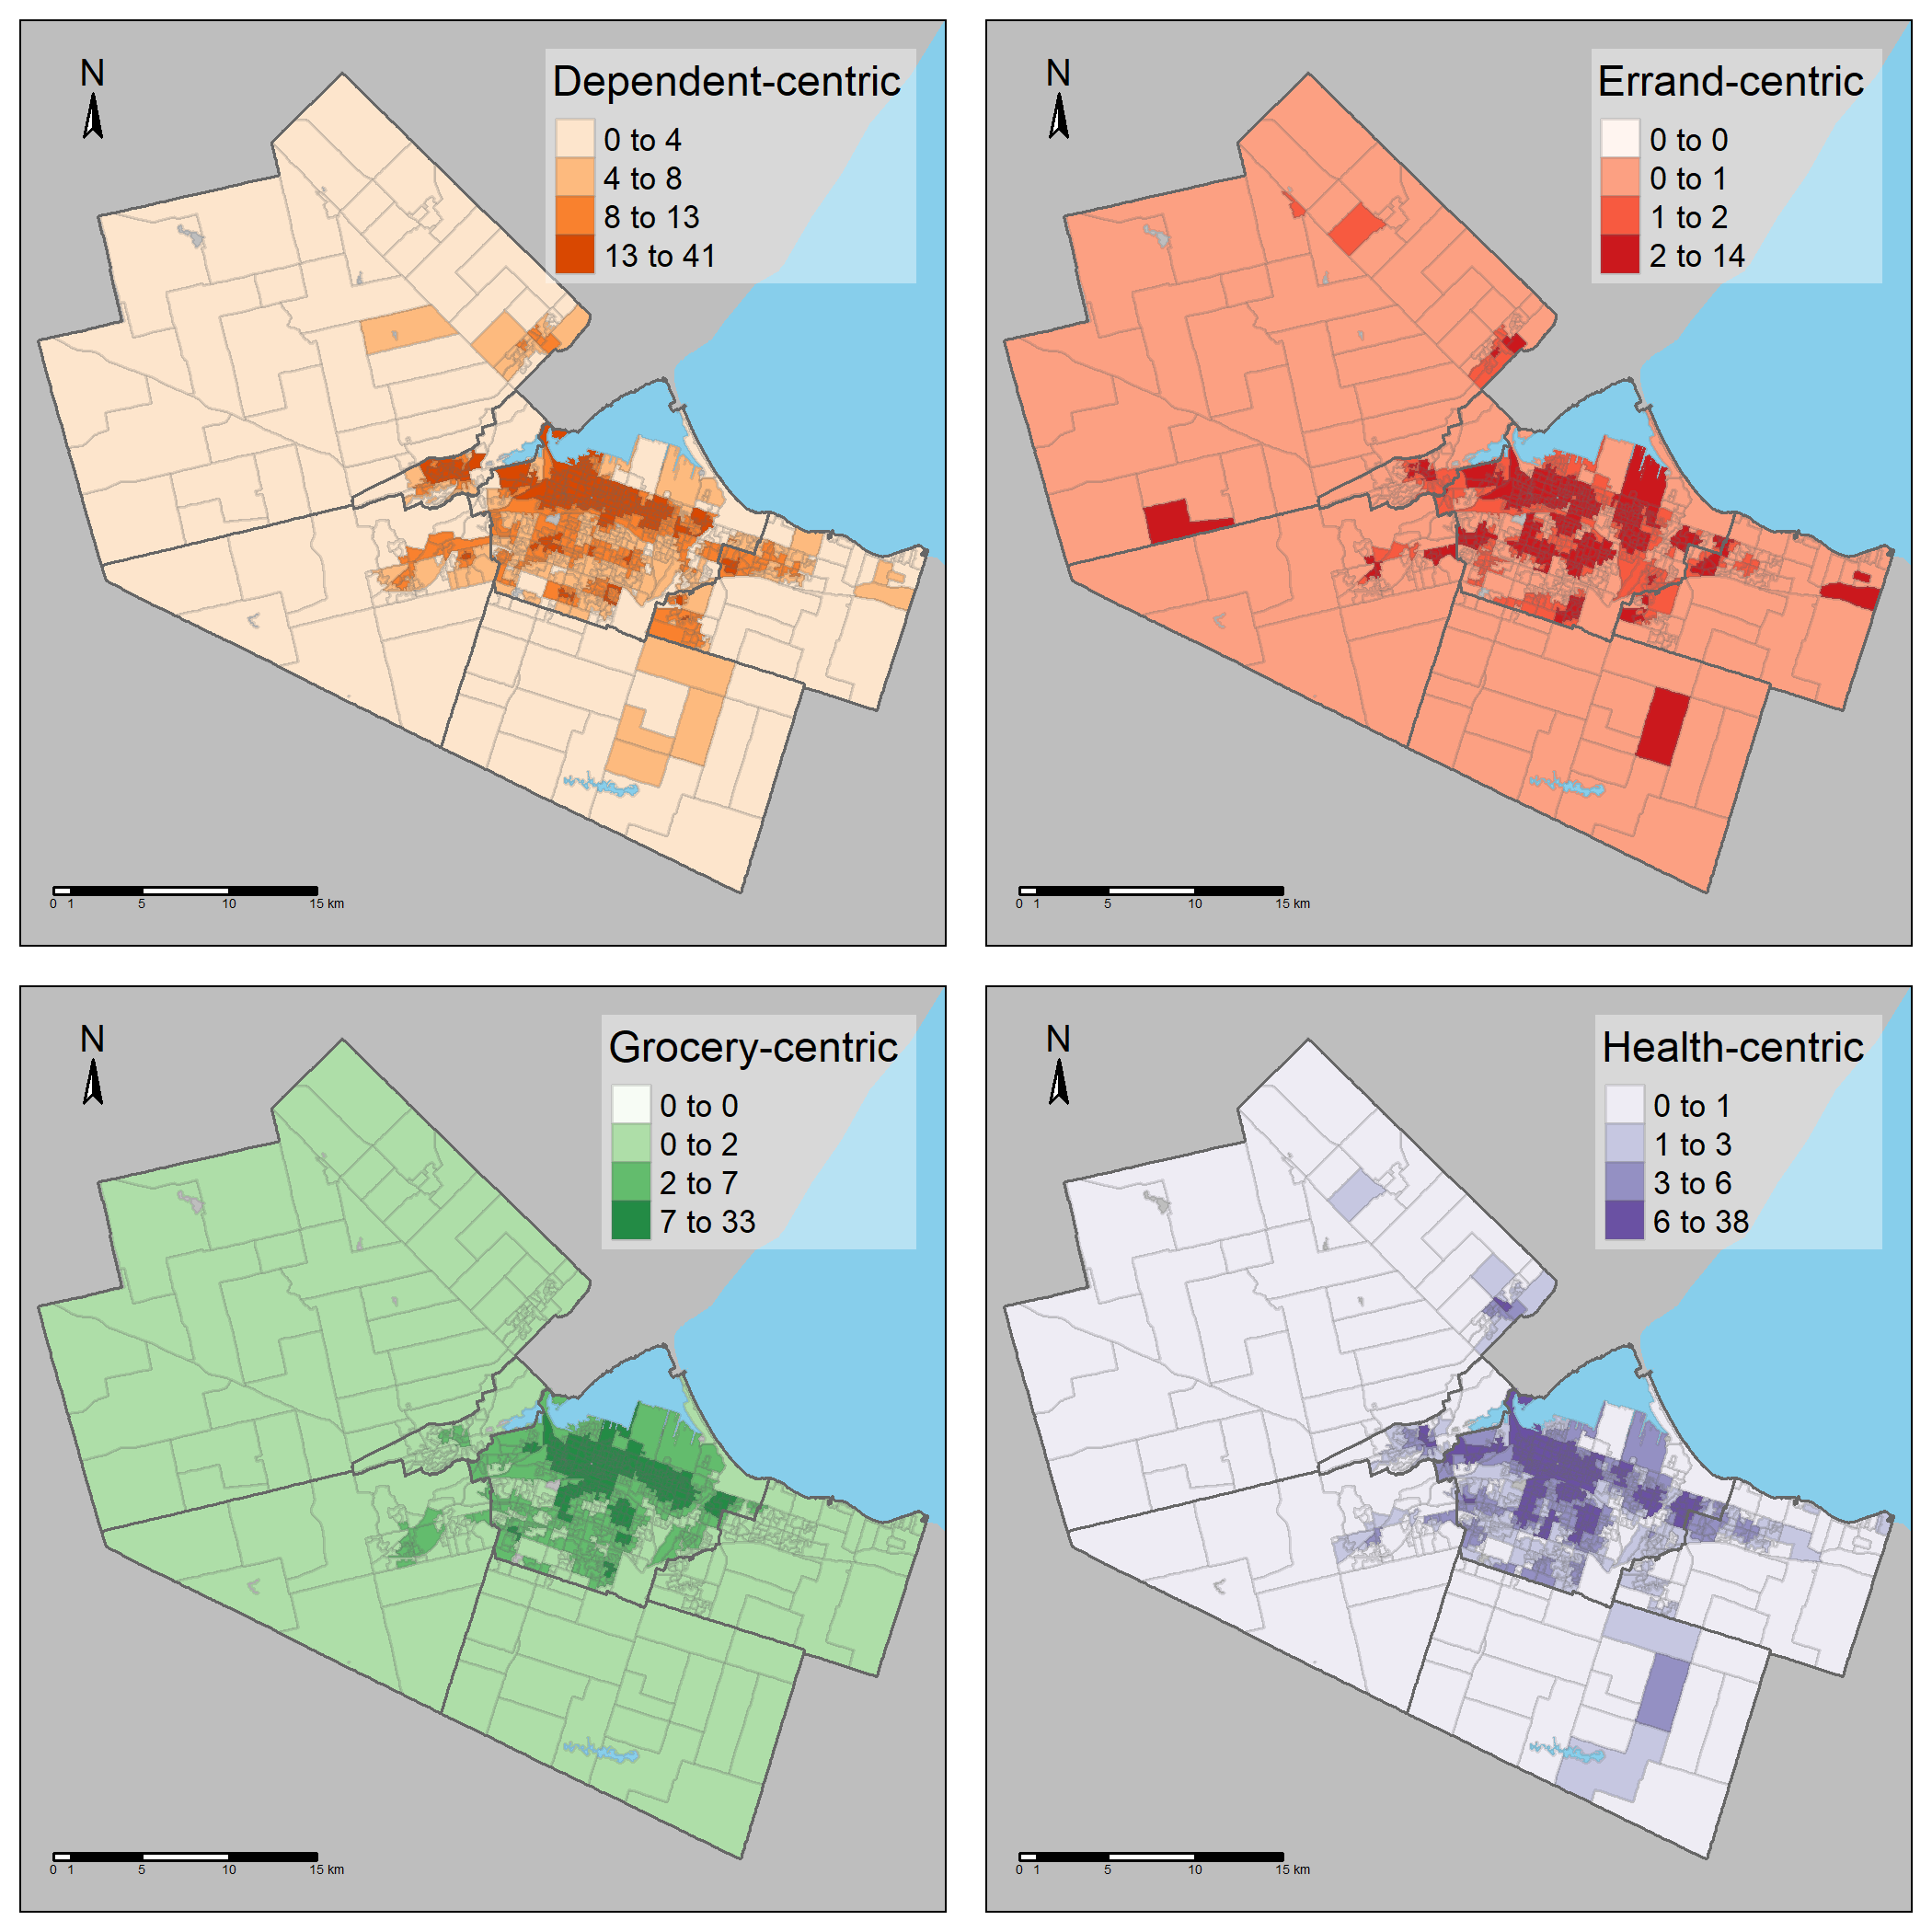
\includegraphics[width=6.25in,height=6.25in]{../figures/percats_copp_plot.png}

}

\caption{\label{fig-Fig4}The number of care destinations that can be
reached within a 15-min walk per care category for a median parcel in
each DA. The values are a summary of the 14 acessibility scores that
served as inputs into the SOM. Basemap shapefiles are retrieved from the
2021 Canadian census \citep{governmentofcanadaCensusPopulation2023}, the
Open Data Hamilton Portal \citep{opendatahamiltonCityBoundary2023} and
the USGS \citep{greatlakesUSGS2010}.}

\end{figure}%

\begin{figure}

\centering{

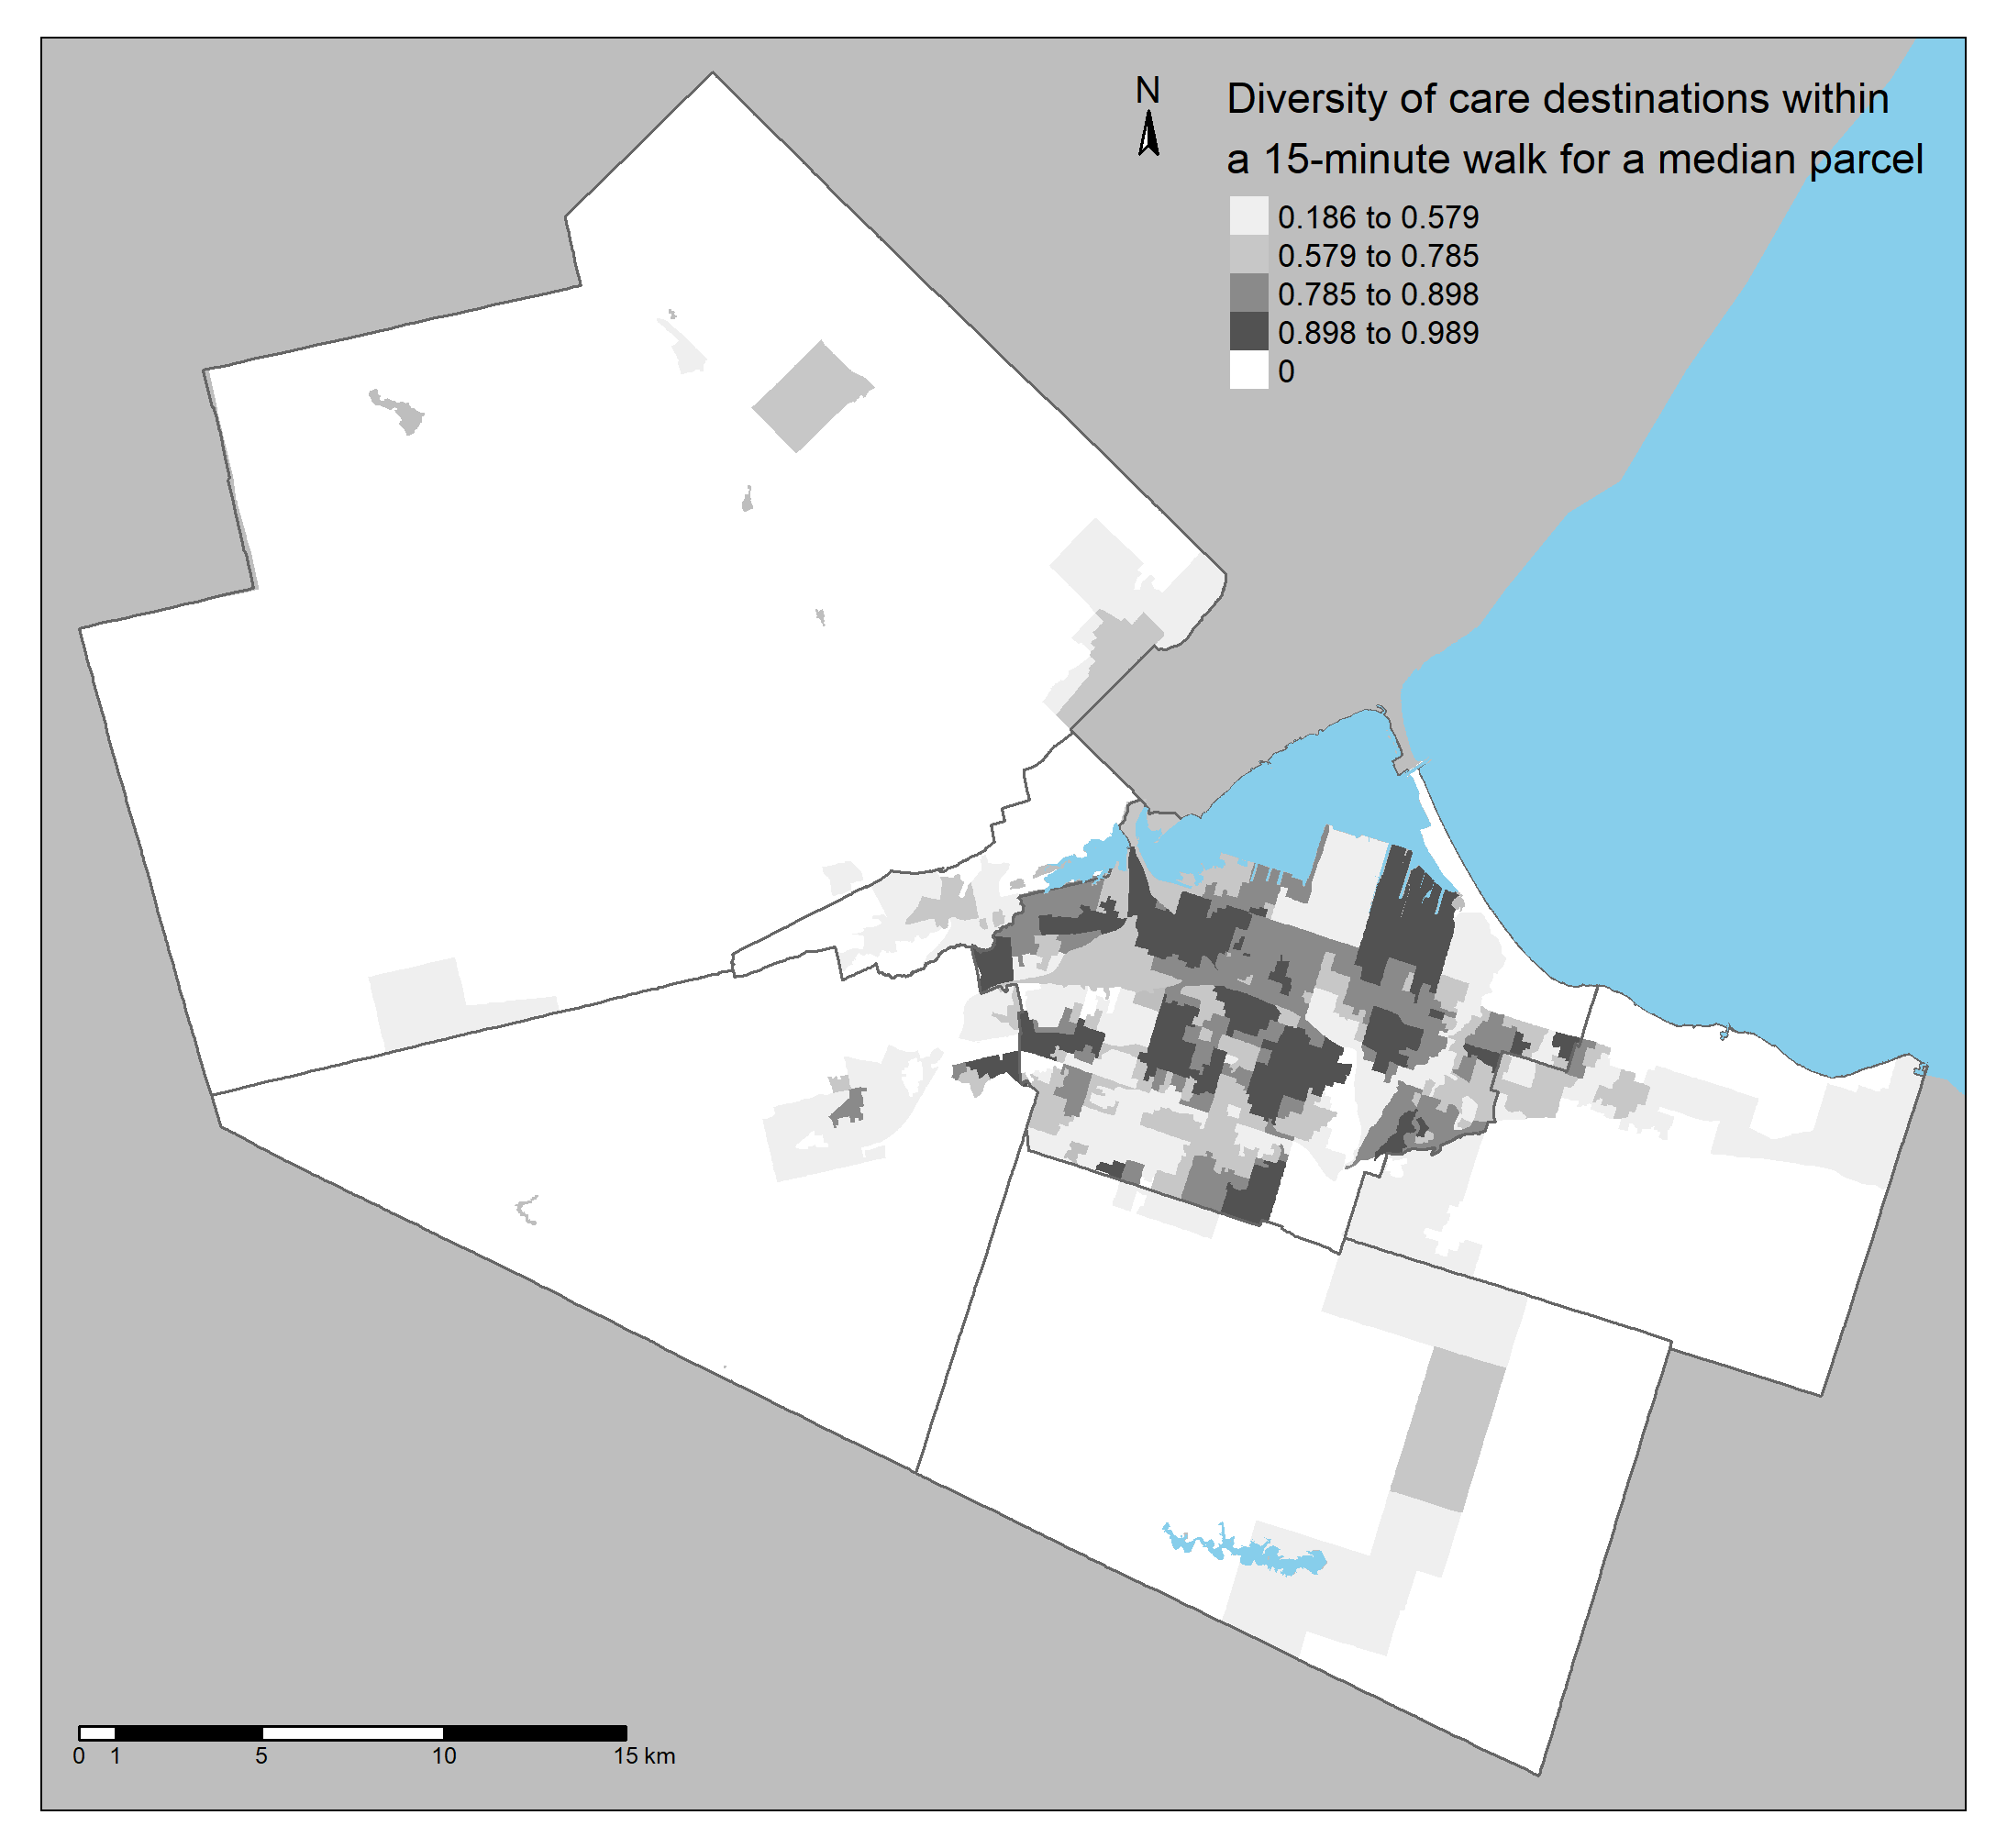
\includegraphics[width=4.6875in,height=4.6875in]{../figures/all_cats_entropy_copp_plot.png}

}

\caption{\label{fig-Fig5}The diversity measure based on the proportion
of care category accessibility in Figure 4. These values are also a
summary of the 15th input into the SOM. Basemap shapefiles are retrieved
from the 2021 Canadian census
\citep{governmentofcanadaCensusPopulation2023}, the Open Data Hamilton
Portal \citep{opendatahamiltonCityBoundary2023} and the USGS
\citep{greatlakesUSGS2010}.}

\end{figure}%

\newpage

\subsection{Identification of completely caring 15-minute neighbourhood
typologies}\label{identification-of-completely-caring-15-minute-neighbourhood-typologies}

In Figure~\ref{fig-Fig4}, the concentration of opportunities for all
category types is centered in the downtown of Hamilton, with the highest
concentration being in the lower city (near the lake shore) and pockets
of the high concentration further from the shoreline. Grocery-centric
destinations appear to be the most concentrated, followed by
health-centric and dependent-centric caring destinations. Errand-centric
destinations are the most sprawled. In many ways, Figure~\ref{fig-Fig4}
mirrors the spatial distribution of care destinations
(Figure~\ref{fig-Fig3}) as the range of 15-minutes of travel is small.
In Figure~\ref{fig-Fig5}, areas that have high care accessibility tend
to have high diversity as well, though there are exceptions in pockets
of the city outside the downtown core that have higher diversity but low
levels of accessibility for all care categories. Similarly, there are
areas with low diversity within the downtown core that have only
moderate or high accessibility to certain care destination types.

Based on the SOM methodology discussed, 7 superclusters are identified
from the 10 by 10 grid of SOM nodes. As diagnostics for the selection of
the number of superclusters, the dissimilarity-index-based dendrogram
with the proportion of parcels represented in each supercluster
alongside the variance explained plot is visualised in
Figure~\ref{fig-Fig6}. Labels representing grades A to D qualifying the
7 superclusters are then assigned. These grades as also reflected in
Figure~\ref{fig-Fig6} and represent the quantity of accessibility and
diversity in accessibility per care category. Higher grades (A+ and A)
corresponding to the highest accessibility and diversity, while lowest
grades (D) representing lowest accessibility and diversity scores.

\begin{figure}

\centering{

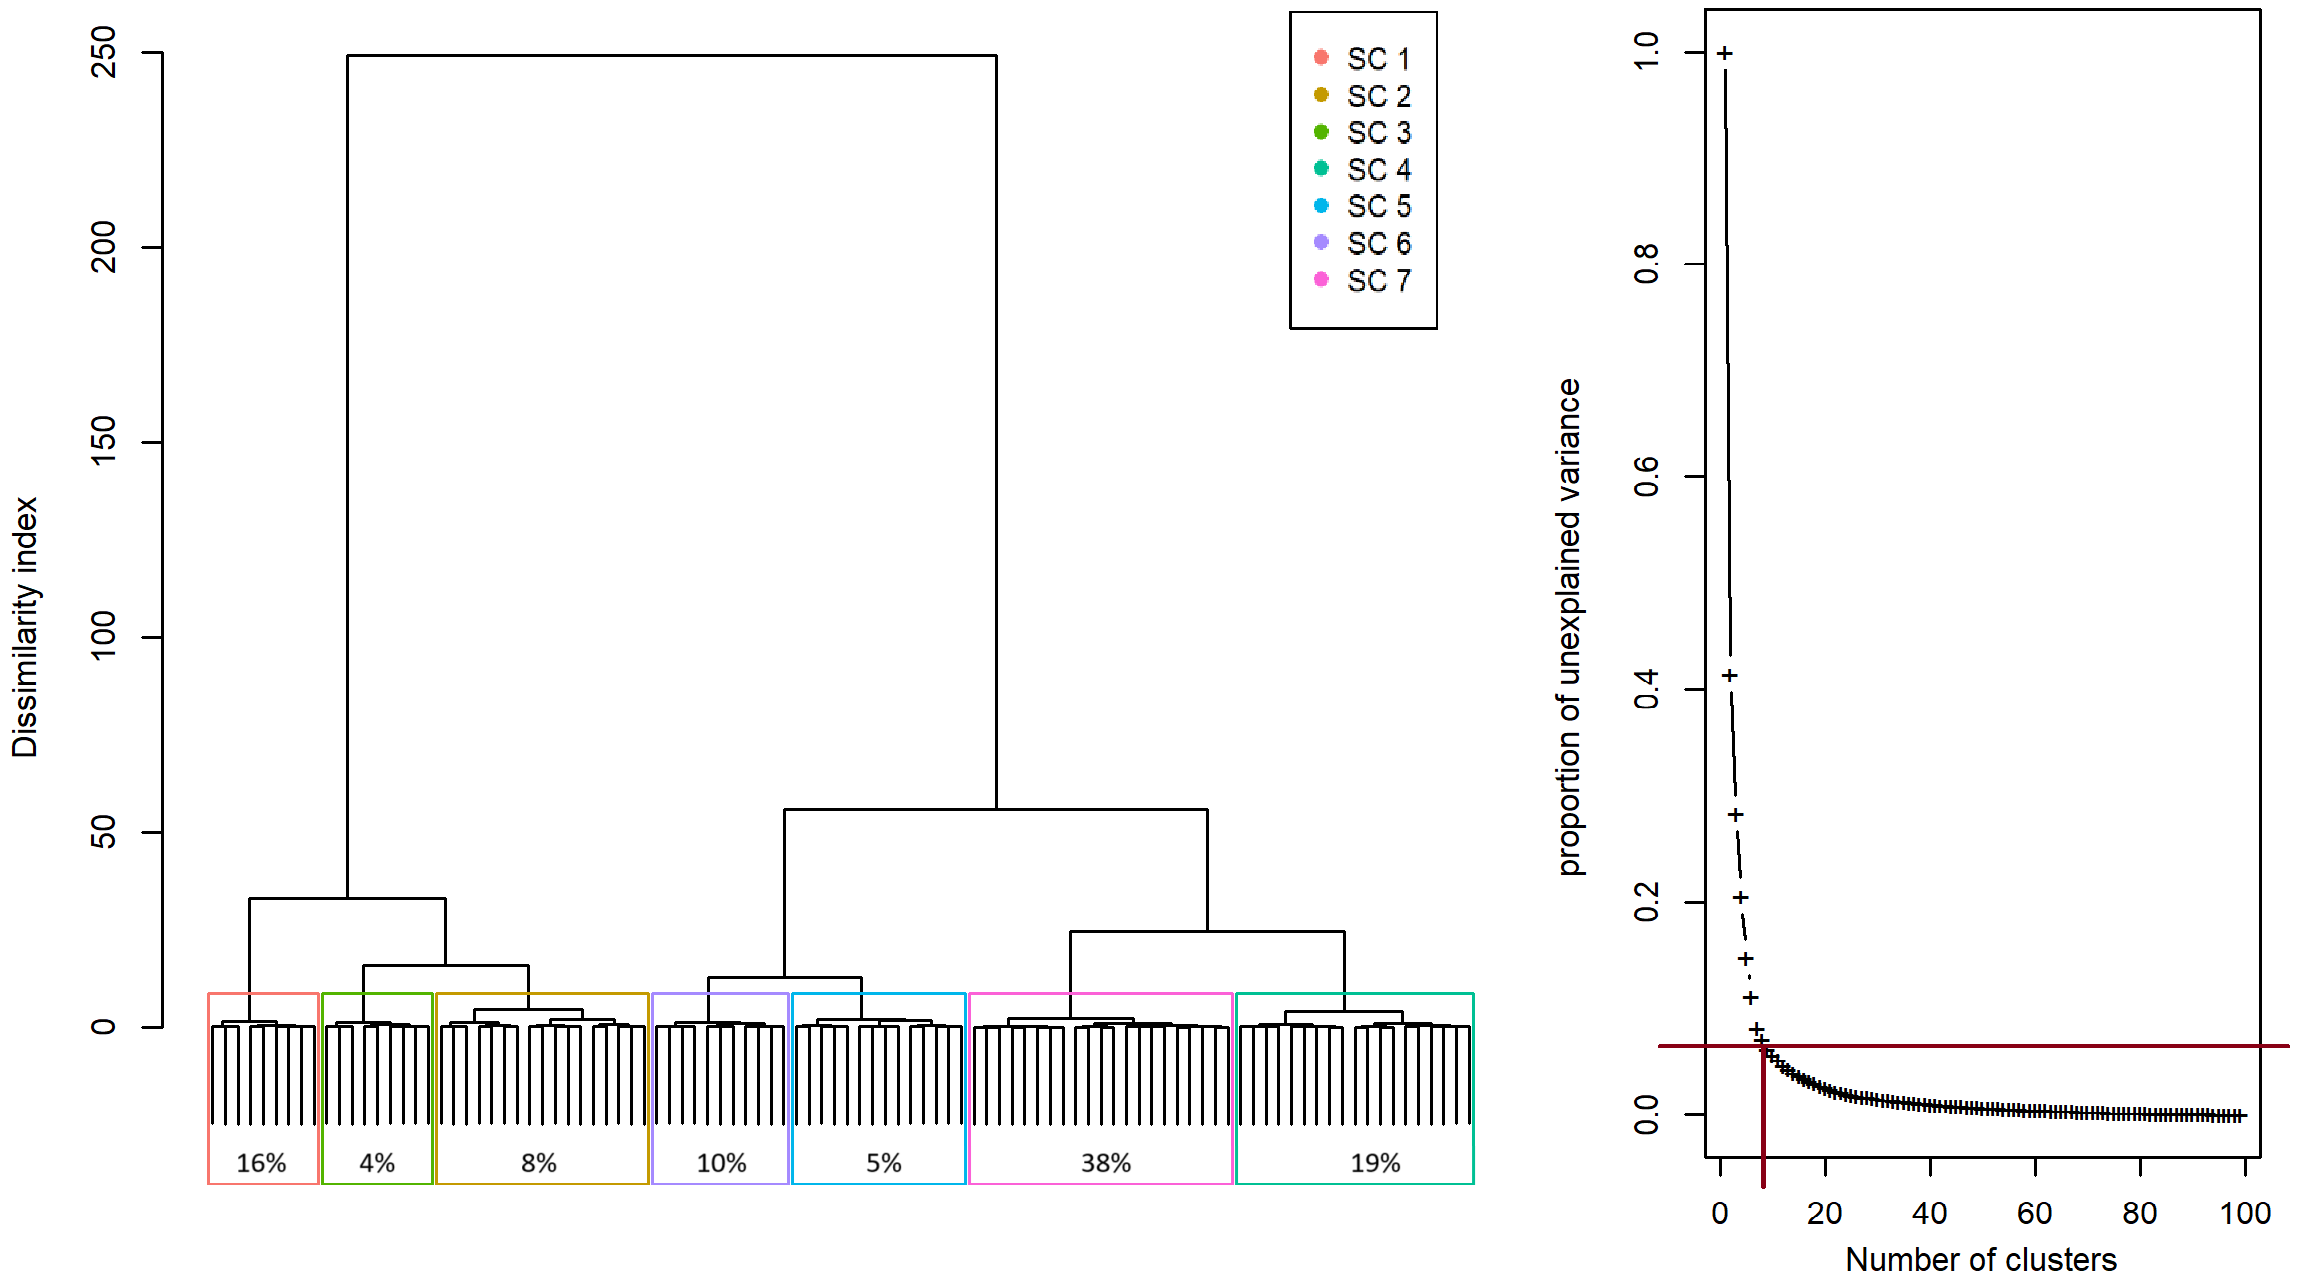
\includegraphics[width=1\textwidth,height=1\textheight]{../figures/all_access_sc_plot_small.png}

}

\caption{\label{fig-Fig6}The 7 resulting superclusters from the SOM the
10 by 10 grid output represented in a dendrogram (left) and the
proportion of variance unexplained by cluster (right).}

\end{figure}%

\newpage

The grade for each supercluster was carefully assigned by the authors by
referring to descriptive statistics and their notable trends. These
statistics are summarised in Table~\ref{tbl-Tbl2} and in the boxplots in
Figure~\ref{fig-Fig7}.

\begin{itemize}
\tightlist
\item
  A+ and A have exceptionally high caring accessibility for all
  destination types and high diversity scores in the top quantile or
  above. Together, these grades represent 24\% of all parcels in the
  city.
\item
  A- has high caring accessibility, but low diversity. Interestingly, A-
  is like A but with much higher dependent-centric destinations,
  particularly parks, schools, and daycares, with only moderately high
  scores for all other destination types. This disbalance lowers its
  overall diversity score. However, it can be characterized as a
  supercluster that demonstrates potential in being retrofitted to
  provide A+ or A level of completely caring access. 4\% of all parcels
  are represented by the A- grade.
\item
  B+ and B superclusters present about average completely caring access.
  These superclusters can serve as the benchmark for what `average'
  completely caring access in Hamilton currently looks like. These
  grades represent 15\% of all parcels.
\item
  B- provides above average dependent-centric destination access,
  particularly parks, daycares and schools, but below average access to
  other destination types and hence has low diversity scores. B- is like
  A- as it demonstrates complete caring 15-minute potential if
  retrofitted. As these parcels demonstrate caring access to some
  destinations, they may have the potential to be retrofitted to support
  complete access to all caring destination types. This grade represents
  19\% of all parcels.
\item
  D superclusters demonstrate the lowest scores all-around, representing
  room for land-use improvement that addresses complete and caring
  15-minute access. This supercluster characterizes the largest number
  of parcels, representing 38\% of parcels in the city.
\end{itemize}

\global\setlength{\Oldarrayrulewidth}{\arrayrulewidth}

\global\setlength{\Oldtabcolsep}{\tabcolsep}

\setlength{\tabcolsep}{2pt}

\renewcommand*{\arraystretch}{1}



\providecommand{\ascline}[3]{\noalign{\global\arrayrulewidth #1}\arrayrulecolor[HTML]{#2}\cline{#3}}

\begin{longtable}[c]{|p{1.20in}|p{0.60in}|p{0.60in}|p{0.60in}|p{0.60in}|p{0.60in}|p{0.60in}|p{0.60in}|p{0.60in}}

\caption{\label{tbl-Tbl2}Mean and (standard deviation) of each SOM
classified cluster by input variable and additional summary variables.
Variables included in the SOM algorthim are in regular case, while
additional summary variables are indicated by ALL CAPITAL LETERS.}

\tabularnewline

\hhline{>{\arrayrulecolor[HTML]{666666}\global\arrayrulewidth=1.5pt}->{\arrayrulecolor[HTML]{666666}\global\arrayrulewidth=1.5pt}->{\arrayrulecolor[HTML]{666666}\global\arrayrulewidth=1.5pt}->{\arrayrulecolor[HTML]{666666}\global\arrayrulewidth=1.5pt}->{\arrayrulecolor[HTML]{666666}\global\arrayrulewidth=1.5pt}->{\arrayrulecolor[HTML]{666666}\global\arrayrulewidth=1.5pt}->{\arrayrulecolor[HTML]{666666}\global\arrayrulewidth=1.5pt}->{\arrayrulecolor[HTML]{666666}\global\arrayrulewidth=1.5pt}->{\arrayrulecolor[HTML]{666666}\global\arrayrulewidth=1.5pt}-}

\multicolumn{1}{>{\raggedright}m{\dimexpr 1.2in+0\tabcolsep}}{\textcolor[HTML]{000000}{\fontsize{8}{8}\selectfont{\ }}} & \multicolumn{1}{>{\raggedright}m{\dimexpr 0.6in+0\tabcolsep}}{\textcolor[HTML]{000000}{\fontsize{8}{8}\selectfont{A+}}} & \multicolumn{1}{>{\raggedright}m{\dimexpr 0.6in+0\tabcolsep}}{\textcolor[HTML]{000000}{\fontsize{8}{8}\selectfont{A}}} & \multicolumn{1}{>{\raggedright}m{\dimexpr 0.6in+0\tabcolsep}}{\textcolor[HTML]{000000}{\fontsize{8}{8}\selectfont{A-}}} & \multicolumn{1}{>{\raggedright}m{\dimexpr 0.6in+0\tabcolsep}}{\textcolor[HTML]{000000}{\fontsize{8}{8}\selectfont{B+}}} & \multicolumn{1}{>{\raggedright}m{\dimexpr 0.6in+0\tabcolsep}}{\textcolor[HTML]{000000}{\fontsize{8}{8}\selectfont{B}}} & \multicolumn{1}{>{\raggedright}m{\dimexpr 0.6in+0\tabcolsep}}{\textcolor[HTML]{000000}{\fontsize{8}{8}\selectfont{B-}}} & \multicolumn{1}{>{\raggedright}m{\dimexpr 0.6in+0\tabcolsep}}{\textcolor[HTML]{000000}{\fontsize{8}{8}\selectfont{D}}} & \multicolumn{1}{>{\raggedright}m{\dimexpr 0.6in+0\tabcolsep}}{\textcolor[HTML]{000000}{\fontsize{8}{8}\selectfont{TOTAL}}} \\

\noalign{\global\arrayrulewidth 0pt}\arrayrulecolor[HTML]{000000}

\hhline{>{\arrayrulecolor[HTML]{666666}\global\arrayrulewidth=1.5pt}->{\arrayrulecolor[HTML]{666666}\global\arrayrulewidth=1.5pt}->{\arrayrulecolor[HTML]{666666}\global\arrayrulewidth=1.5pt}->{\arrayrulecolor[HTML]{666666}\global\arrayrulewidth=1.5pt}->{\arrayrulecolor[HTML]{666666}\global\arrayrulewidth=1.5pt}->{\arrayrulecolor[HTML]{666666}\global\arrayrulewidth=1.5pt}->{\arrayrulecolor[HTML]{666666}\global\arrayrulewidth=1.5pt}->{\arrayrulecolor[HTML]{666666}\global\arrayrulewidth=1.5pt}->{\arrayrulecolor[HTML]{666666}\global\arrayrulewidth=1.5pt}-}\endfirsthead 

\hhline{>{\arrayrulecolor[HTML]{666666}\global\arrayrulewidth=1.5pt}->{\arrayrulecolor[HTML]{666666}\global\arrayrulewidth=1.5pt}->{\arrayrulecolor[HTML]{666666}\global\arrayrulewidth=1.5pt}->{\arrayrulecolor[HTML]{666666}\global\arrayrulewidth=1.5pt}->{\arrayrulecolor[HTML]{666666}\global\arrayrulewidth=1.5pt}->{\arrayrulecolor[HTML]{666666}\global\arrayrulewidth=1.5pt}->{\arrayrulecolor[HTML]{666666}\global\arrayrulewidth=1.5pt}->{\arrayrulecolor[HTML]{666666}\global\arrayrulewidth=1.5pt}->{\arrayrulecolor[HTML]{666666}\global\arrayrulewidth=1.5pt}-}

\multicolumn{1}{>{\raggedright}m{\dimexpr 1.2in+0\tabcolsep}}{\textcolor[HTML]{000000}{\fontsize{8}{8}\selectfont{\ }}} & \multicolumn{1}{>{\raggedright}m{\dimexpr 0.6in+0\tabcolsep}}{\textcolor[HTML]{000000}{\fontsize{8}{8}\selectfont{A+}}} & \multicolumn{1}{>{\raggedright}m{\dimexpr 0.6in+0\tabcolsep}}{\textcolor[HTML]{000000}{\fontsize{8}{8}\selectfont{A}}} & \multicolumn{1}{>{\raggedright}m{\dimexpr 0.6in+0\tabcolsep}}{\textcolor[HTML]{000000}{\fontsize{8}{8}\selectfont{A-}}} & \multicolumn{1}{>{\raggedright}m{\dimexpr 0.6in+0\tabcolsep}}{\textcolor[HTML]{000000}{\fontsize{8}{8}\selectfont{B+}}} & \multicolumn{1}{>{\raggedright}m{\dimexpr 0.6in+0\tabcolsep}}{\textcolor[HTML]{000000}{\fontsize{8}{8}\selectfont{B}}} & \multicolumn{1}{>{\raggedright}m{\dimexpr 0.6in+0\tabcolsep}}{\textcolor[HTML]{000000}{\fontsize{8}{8}\selectfont{B-}}} & \multicolumn{1}{>{\raggedright}m{\dimexpr 0.6in+0\tabcolsep}}{\textcolor[HTML]{000000}{\fontsize{8}{8}\selectfont{D}}} & \multicolumn{1}{>{\raggedright}m{\dimexpr 0.6in+0\tabcolsep}}{\textcolor[HTML]{000000}{\fontsize{8}{8}\selectfont{TOTAL}}} \\

\noalign{\global\arrayrulewidth 0pt}\arrayrulecolor[HTML]{000000}

\hhline{>{\arrayrulecolor[HTML]{666666}\global\arrayrulewidth=1.5pt}->{\arrayrulecolor[HTML]{666666}\global\arrayrulewidth=1.5pt}->{\arrayrulecolor[HTML]{666666}\global\arrayrulewidth=1.5pt}->{\arrayrulecolor[HTML]{666666}\global\arrayrulewidth=1.5pt}->{\arrayrulecolor[HTML]{666666}\global\arrayrulewidth=1.5pt}->{\arrayrulecolor[HTML]{666666}\global\arrayrulewidth=1.5pt}->{\arrayrulecolor[HTML]{666666}\global\arrayrulewidth=1.5pt}->{\arrayrulecolor[HTML]{666666}\global\arrayrulewidth=1.5pt}->{\arrayrulecolor[HTML]{666666}\global\arrayrulewidth=1.5pt}-}\endhead



\multicolumn{1}{>{\raggedright}m{\dimexpr 1.2in+0\tabcolsep}}{\textcolor[HTML]{000000}{\fontsize{8}{0}\selectfont{GROCERY}}\textcolor[HTML]{000000}{\fontsize{8}{0}\selectfont{\ }}\textcolor[HTML]{000000}{\fontsize{8}{0}\selectfont{TOTALS}}} & \multicolumn{1}{>{\cellcolor[HTML]{48B376}\raggedright}m{\dimexpr 0.6in+0\tabcolsep}}{\textcolor[HTML]{000000}{\fontsize{8}{0}\selectfont{12.2}}\textcolor[HTML]{000000}{\fontsize{8}{0}\selectfont{\ }}\textcolor[HTML]{000000}{\fontsize{8}{0}\selectfont{(5.7)}}} & \multicolumn{1}{>{\cellcolor[HTML]{91CF60}\raggedright}m{\dimexpr 0.6in+0\tabcolsep}}{\textcolor[HTML]{000000}{\fontsize{8}{0}\selectfont{7}}\textcolor[HTML]{000000}{\fontsize{8}{0}\selectfont{\ }}\textcolor[HTML]{000000}{\fontsize{8}{0}\selectfont{(3.1)}}} & \multicolumn{1}{>{\cellcolor[HTML]{D9EF8B}\raggedright}m{\dimexpr 0.6in+0\tabcolsep}}{\textcolor[HTML]{000000}{\fontsize{8}{0}\selectfont{2.8}}\textcolor[HTML]{000000}{\fontsize{8}{0}\selectfont{\ }}\textcolor[HTML]{000000}{\fontsize{8}{0}\selectfont{(2.6)}}} & \multicolumn{1}{>{\cellcolor[HTML]{FFFFBF}\raggedright}m{\dimexpr 0.6in+0\tabcolsep}}{\textcolor[HTML]{000000}{\fontsize{8}{0}\selectfont{4.8}}\textcolor[HTML]{000000}{\fontsize{8}{0}\selectfont{\ }}\textcolor[HTML]{000000}{\fontsize{8}{0}\selectfont{(2.5)}}} & \multicolumn{1}{>{\cellcolor[HTML]{FEE08B}\raggedright}m{\dimexpr 0.6in+0\tabcolsep}}{\textcolor[HTML]{000000}{\fontsize{8}{0}\selectfont{2.7}}\textcolor[HTML]{000000}{\fontsize{8}{0}\selectfont{\ }}\textcolor[HTML]{000000}{\fontsize{8}{0}\selectfont{(2.2)}}} & \multicolumn{1}{>{\cellcolor[HTML]{FDAE61}\raggedright}m{\dimexpr 0.6in+0\tabcolsep}}{\textcolor[HTML]{000000}{\fontsize{8}{0}\selectfont{1}}\textcolor[HTML]{000000}{\fontsize{8}{0}\selectfont{\ }}\textcolor[HTML]{000000}{\fontsize{8}{0}\selectfont{(1.6)}}} & \multicolumn{1}{>{\cellcolor[HTML]{D75C56}\raggedright}m{\dimexpr 0.6in+0\tabcolsep}}{\textcolor[HTML]{000000}{\fontsize{8}{0}\selectfont{0.5}}\textcolor[HTML]{000000}{\fontsize{8}{0}\selectfont{\ }}\textcolor[HTML]{000000}{\fontsize{8}{0}\selectfont{(1.2)}}} & \multicolumn{1}{>{\raggedright}m{\dimexpr 0.6in+0\tabcolsep}}{\textcolor[HTML]{000000}{\fontsize{8}{0}\selectfont{3.6}}\textcolor[HTML]{000000}{\fontsize{8}{0}\selectfont{\ }}\textcolor[HTML]{000000}{\fontsize{8}{0}\selectfont{(5.1)}}} \\

\noalign{\global\arrayrulewidth 0pt}\arrayrulecolor[HTML]{000000}





\multicolumn{1}{>{\raggedright}m{\dimexpr 1.2in+0\tabcolsep}}{\textcolor[HTML]{000000}{\fontsize{8}{0}\selectfont{Convenience}}\textcolor[HTML]{000000}{\fontsize{8}{0}\selectfont{\ }}\textcolor[HTML]{000000}{\fontsize{8}{0}\selectfont{Store}}} & \multicolumn{1}{>{\cellcolor[HTML]{48B376}\raggedright}m{\dimexpr 0.6in+0\tabcolsep}}{\textcolor[HTML]{000000}{\fontsize{8}{0}\selectfont{8}}\textcolor[HTML]{000000}{\fontsize{8}{0}\selectfont{\ }}\textcolor[HTML]{000000}{\fontsize{8}{0}\selectfont{(4)}}} & \multicolumn{1}{>{\cellcolor[HTML]{91CF60}\raggedright}m{\dimexpr 0.6in+0\tabcolsep}}{\textcolor[HTML]{000000}{\fontsize{8}{0}\selectfont{4.5}}\textcolor[HTML]{000000}{\fontsize{8}{0}\selectfont{\ }}\textcolor[HTML]{000000}{\fontsize{8}{0}\selectfont{(2.6)}}} & \multicolumn{1}{>{\cellcolor[HTML]{D9EF8B}\raggedright}m{\dimexpr 0.6in+0\tabcolsep}}{\textcolor[HTML]{000000}{\fontsize{8}{0}\selectfont{2}}\textcolor[HTML]{000000}{\fontsize{8}{0}\selectfont{\ }}\textcolor[HTML]{000000}{\fontsize{8}{0}\selectfont{(2.1)}}} & \multicolumn{1}{>{\cellcolor[HTML]{FFFFBF}\raggedright}m{\dimexpr 0.6in+0\tabcolsep}}{\textcolor[HTML]{000000}{\fontsize{8}{0}\selectfont{3}}\textcolor[HTML]{000000}{\fontsize{8}{0}\selectfont{\ }}\textcolor[HTML]{000000}{\fontsize{8}{0}\selectfont{(1.9)}}} & \multicolumn{1}{>{\cellcolor[HTML]{FEE08B}\raggedright}m{\dimexpr 0.6in+0\tabcolsep}}{\textcolor[HTML]{000000}{\fontsize{8}{0}\selectfont{1.8}}\textcolor[HTML]{000000}{\fontsize{8}{0}\selectfont{\ }}\textcolor[HTML]{000000}{\fontsize{8}{0}\selectfont{(1.6)}}} & \multicolumn{1}{>{\cellcolor[HTML]{FDAE61}\raggedright}m{\dimexpr 0.6in+0\tabcolsep}}{\textcolor[HTML]{000000}{\fontsize{8}{0}\selectfont{0.8}}\textcolor[HTML]{000000}{\fontsize{8}{0}\selectfont{\ }}\textcolor[HTML]{000000}{\fontsize{8}{0}\selectfont{(1.2)}}} & \multicolumn{1}{>{\cellcolor[HTML]{D75C56}\raggedright}m{\dimexpr 0.6in+0\tabcolsep}}{\textcolor[HTML]{000000}{\fontsize{8}{0}\selectfont{0.4}}\textcolor[HTML]{000000}{\fontsize{8}{0}\selectfont{\ }}\textcolor[HTML]{000000}{\fontsize{8}{0}\selectfont{(0.9)}}} & \multicolumn{1}{>{\raggedright}m{\dimexpr 0.6in+0\tabcolsep}}{\textcolor[HTML]{000000}{\fontsize{8}{0}\selectfont{2.4}}\textcolor[HTML]{000000}{\fontsize{8}{0}\selectfont{\ }}\textcolor[HTML]{000000}{\fontsize{8}{0}\selectfont{(3.4)}}} \\

\noalign{\global\arrayrulewidth 0pt}\arrayrulecolor[HTML]{000000}





\multicolumn{1}{>{\raggedright}m{\dimexpr 1.2in+0\tabcolsep}}{\textcolor[HTML]{000000}{\fontsize{8}{0}\selectfont{Grocer}}} & \multicolumn{1}{>{\cellcolor[HTML]{48B376}\raggedright}m{\dimexpr 0.6in+0\tabcolsep}}{\textcolor[HTML]{000000}{\fontsize{8}{0}\selectfont{4.2}}\textcolor[HTML]{000000}{\fontsize{8}{0}\selectfont{\ }}\textcolor[HTML]{000000}{\fontsize{8}{0}\selectfont{(2.8)}}} & \multicolumn{1}{>{\cellcolor[HTML]{91CF60}\raggedright}m{\dimexpr 0.6in+0\tabcolsep}}{\textcolor[HTML]{000000}{\fontsize{8}{0}\selectfont{2.6}}\textcolor[HTML]{000000}{\fontsize{8}{0}\selectfont{\ }}\textcolor[HTML]{000000}{\fontsize{8}{0}\selectfont{(1.5)}}} & \multicolumn{1}{>{\cellcolor[HTML]{D9EF8B}\raggedright}m{\dimexpr 0.6in+0\tabcolsep}}{\textcolor[HTML]{000000}{\fontsize{8}{0}\selectfont{0.7}}\textcolor[HTML]{000000}{\fontsize{8}{0}\selectfont{\ }}\textcolor[HTML]{000000}{\fontsize{8}{0}\selectfont{(0.9)}}} & \multicolumn{1}{>{\cellcolor[HTML]{FFFFBF}\raggedright}m{\dimexpr 0.6in+0\tabcolsep}}{\textcolor[HTML]{000000}{\fontsize{8}{0}\selectfont{1.9}}\textcolor[HTML]{000000}{\fontsize{8}{0}\selectfont{\ }}\textcolor[HTML]{000000}{\fontsize{8}{0}\selectfont{(1.2)}}} & \multicolumn{1}{>{\cellcolor[HTML]{FEE08B}\raggedright}m{\dimexpr 0.6in+0\tabcolsep}}{\textcolor[HTML]{000000}{\fontsize{8}{0}\selectfont{0.9}}\textcolor[HTML]{000000}{\fontsize{8}{0}\selectfont{\ }}\textcolor[HTML]{000000}{\fontsize{8}{0}\selectfont{(1)}}} & \multicolumn{1}{>{\cellcolor[HTML]{FDAE61}\raggedright}m{\dimexpr 0.6in+0\tabcolsep}}{\textcolor[HTML]{000000}{\fontsize{8}{0}\selectfont{0.2}}\textcolor[HTML]{000000}{\fontsize{8}{0}\selectfont{\ }}\textcolor[HTML]{000000}{\fontsize{8}{0}\selectfont{(0.6)}}} & \multicolumn{1}{>{\cellcolor[HTML]{D75C56}\raggedright}m{\dimexpr 0.6in+0\tabcolsep}}{\textcolor[HTML]{000000}{\fontsize{8}{0}\selectfont{0.1}}\textcolor[HTML]{000000}{\fontsize{8}{0}\selectfont{\ }}\textcolor[HTML]{000000}{\fontsize{8}{0}\selectfont{(0.4)}}} & \multicolumn{1}{>{\raggedright}m{\dimexpr 0.6in+0\tabcolsep}}{\textcolor[HTML]{000000}{\fontsize{8}{0}\selectfont{1.2}}\textcolor[HTML]{000000}{\fontsize{8}{0}\selectfont{\ }}\textcolor[HTML]{000000}{\fontsize{8}{0}\selectfont{(2)}}} \\

\noalign{\global\arrayrulewidth 0pt}\arrayrulecolor[HTML]{000000}

\hhline{>{\arrayrulecolor[HTML]{666666}\global\arrayrulewidth=1pt}->{\arrayrulecolor[HTML]{666666}\global\arrayrulewidth=1pt}->{\arrayrulecolor[HTML]{666666}\global\arrayrulewidth=1pt}->{\arrayrulecolor[HTML]{666666}\global\arrayrulewidth=1pt}->{\arrayrulecolor[HTML]{666666}\global\arrayrulewidth=1pt}->{\arrayrulecolor[HTML]{666666}\global\arrayrulewidth=1pt}->{\arrayrulecolor[HTML]{666666}\global\arrayrulewidth=1pt}->{\arrayrulecolor[HTML]{666666}\global\arrayrulewidth=1pt}->{\arrayrulecolor[HTML]{666666}\global\arrayrulewidth=1pt}-}



\multicolumn{1}{>{\raggedright}m{\dimexpr 1.2in+0\tabcolsep}}{\textcolor[HTML]{000000}{\fontsize{8}{0}\selectfont{DEP.}}\textcolor[HTML]{000000}{\fontsize{8}{0}\selectfont{\ }}\textcolor[HTML]{000000}{\fontsize{8}{0}\selectfont{TOTALS}}} & \multicolumn{1}{>{\cellcolor[HTML]{48B376}\raggedright}m{\dimexpr 0.6in+0\tabcolsep}}{\textcolor[HTML]{000000}{\fontsize{8}{0}\selectfont{17.5}}\textcolor[HTML]{000000}{\fontsize{8}{0}\selectfont{\ }}\textcolor[HTML]{000000}{\fontsize{8}{0}\selectfont{(5.8)}}} & \multicolumn{1}{>{\cellcolor[HTML]{91CF60}\raggedright}m{\dimexpr 0.6in+0\tabcolsep}}{\textcolor[HTML]{000000}{\fontsize{8}{0}\selectfont{11.5}}\textcolor[HTML]{000000}{\fontsize{8}{0}\selectfont{\ }}\textcolor[HTML]{000000}{\fontsize{8}{0}\selectfont{(4.3)}}} & \multicolumn{1}{>{\cellcolor[HTML]{D9EF8B}\raggedright}m{\dimexpr 0.6in+0\tabcolsep}}{\textcolor[HTML]{000000}{\fontsize{8}{0}\selectfont{13.4}}\textcolor[HTML]{000000}{\fontsize{8}{0}\selectfont{\ }}\textcolor[HTML]{000000}{\fontsize{8}{0}\selectfont{(3)}}} & \multicolumn{1}{>{\cellcolor[HTML]{FFFFBF}\raggedright}m{\dimexpr 0.6in+0\tabcolsep}}{\textcolor[HTML]{000000}{\fontsize{8}{0}\selectfont{6.7}}\textcolor[HTML]{000000}{\fontsize{8}{0}\selectfont{\ }}\textcolor[HTML]{000000}{\fontsize{8}{0}\selectfont{(2.4)}}} & \multicolumn{1}{>{\cellcolor[HTML]{FEE08B}\raggedright}m{\dimexpr 0.6in+0\tabcolsep}}{\textcolor[HTML]{000000}{\fontsize{8}{0}\selectfont{5.3}}\textcolor[HTML]{000000}{\fontsize{8}{0}\selectfont{\ }}\textcolor[HTML]{000000}{\fontsize{8}{0}\selectfont{(2.4)}}} & \multicolumn{1}{>{\cellcolor[HTML]{FDAE61}\raggedright}m{\dimexpr 0.6in+0\tabcolsep}}{\textcolor[HTML]{000000}{\fontsize{8}{0}\selectfont{9.5}}\textcolor[HTML]{000000}{\fontsize{8}{0}\selectfont{\ }}\textcolor[HTML]{000000}{\fontsize{8}{0}\selectfont{(2.4)}}} & \multicolumn{1}{>{\cellcolor[HTML]{D75C56}\raggedright}m{\dimexpr 0.6in+0\tabcolsep}}{\textcolor[HTML]{000000}{\fontsize{8}{0}\selectfont{2.9}}\textcolor[HTML]{000000}{\fontsize{8}{0}\selectfont{\ }}\textcolor[HTML]{000000}{\fontsize{8}{0}\selectfont{(2.1)}}} & \multicolumn{1}{>{\raggedright}m{\dimexpr 0.6in+0\tabcolsep}}{\textcolor[HTML]{000000}{\fontsize{8}{0}\selectfont{8.1}}\textcolor[HTML]{000000}{\fontsize{8}{0}\selectfont{\ }}\textcolor[HTML]{000000}{\fontsize{8}{0}\selectfont{(6.2)}}} \\

\noalign{\global\arrayrulewidth 0pt}\arrayrulecolor[HTML]{000000}





\multicolumn{1}{>{\raggedright}m{\dimexpr 1.2in+0\tabcolsep}}{\textcolor[HTML]{000000}{\fontsize{8}{0}\selectfont{Comm.}}\textcolor[HTML]{000000}{\fontsize{8}{0}\selectfont{\ }}\textcolor[HTML]{000000}{\fontsize{8}{0}\selectfont{or}}\textcolor[HTML]{000000}{\fontsize{8}{0}\selectfont{\ }}\textcolor[HTML]{000000}{\fontsize{8}{0}\selectfont{Rec.}}\textcolor[HTML]{000000}{\fontsize{8}{0}\selectfont{\ }}\textcolor[HTML]{000000}{\fontsize{8}{0}\selectfont{centre}}} & \multicolumn{1}{>{\cellcolor[HTML]{48B376}\raggedright}m{\dimexpr 0.6in+0\tabcolsep}}{\textcolor[HTML]{000000}{\fontsize{8}{0}\selectfont{1.3}}\textcolor[HTML]{000000}{\fontsize{8}{0}\selectfont{\ }}\textcolor[HTML]{000000}{\fontsize{8}{0}\selectfont{(1)}}} & \multicolumn{1}{>{\cellcolor[HTML]{91CF60}\raggedright}m{\dimexpr 0.6in+0\tabcolsep}}{\textcolor[HTML]{000000}{\fontsize{8}{0}\selectfont{0.7}}\textcolor[HTML]{000000}{\fontsize{8}{0}\selectfont{\ }}\textcolor[HTML]{000000}{\fontsize{8}{0}\selectfont{(0.9)}}} & \multicolumn{1}{>{\cellcolor[HTML]{D9EF8B}\raggedright}m{\dimexpr 0.6in+0\tabcolsep}}{\textcolor[HTML]{000000}{\fontsize{8}{0}\selectfont{1}}\textcolor[HTML]{000000}{\fontsize{8}{0}\selectfont{\ }}\textcolor[HTML]{000000}{\fontsize{8}{0}\selectfont{(0.8)}}} & \multicolumn{1}{>{\cellcolor[HTML]{FFFFBF}\raggedright}m{\dimexpr 0.6in+0\tabcolsep}}{\textcolor[HTML]{000000}{\fontsize{8}{0}\selectfont{0.2}}\textcolor[HTML]{000000}{\fontsize{8}{0}\selectfont{\ }}\textcolor[HTML]{000000}{\fontsize{8}{0}\selectfont{(0.4)}}} & \multicolumn{1}{>{\cellcolor[HTML]{FEE08B}\raggedright}m{\dimexpr 0.6in+0\tabcolsep}}{\textcolor[HTML]{000000}{\fontsize{8}{0}\selectfont{0.2}}\textcolor[HTML]{000000}{\fontsize{8}{0}\selectfont{\ }}\textcolor[HTML]{000000}{\fontsize{8}{0}\selectfont{(0.4)}}} & \multicolumn{1}{>{\cellcolor[HTML]{FDAE61}\raggedright}m{\dimexpr 0.6in+0\tabcolsep}}{\textcolor[HTML]{000000}{\fontsize{8}{0}\selectfont{0.4}}\textcolor[HTML]{000000}{\fontsize{8}{0}\selectfont{\ }}\textcolor[HTML]{000000}{\fontsize{8}{0}\selectfont{(0.6)}}} & \multicolumn{1}{>{\cellcolor[HTML]{D75C56}\raggedright}m{\dimexpr 0.6in+0\tabcolsep}}{\textcolor[HTML]{000000}{\fontsize{8}{0}\selectfont{0.1}}\textcolor[HTML]{000000}{\fontsize{8}{0}\selectfont{\ }}\textcolor[HTML]{000000}{\fontsize{8}{0}\selectfont{(0.3)}}} & \multicolumn{1}{>{\raggedright}m{\dimexpr 0.6in+0\tabcolsep}}{\textcolor[HTML]{000000}{\fontsize{8}{0}\selectfont{0.4}}\textcolor[HTML]{000000}{\fontsize{8}{0}\selectfont{\ }}\textcolor[HTML]{000000}{\fontsize{8}{0}\selectfont{(0.8)}}} \\

\noalign{\global\arrayrulewidth 0pt}\arrayrulecolor[HTML]{000000}





\multicolumn{1}{>{\raggedright}m{\dimexpr 1.2in+0\tabcolsep}}{\textcolor[HTML]{000000}{\fontsize{8}{0}\selectfont{Daycare}}\textcolor[HTML]{000000}{\fontsize{8}{0}\selectfont{\ }}\textcolor[HTML]{000000}{\fontsize{8}{0}\selectfont{or}}\textcolor[HTML]{000000}{\fontsize{8}{0}\selectfont{\ }}\textcolor[HTML]{000000}{\fontsize{8}{0}\selectfont{EarlyON}}} & \multicolumn{1}{>{\cellcolor[HTML]{48B376}\raggedright}m{\dimexpr 0.6in+0\tabcolsep}}{\textcolor[HTML]{000000}{\fontsize{8}{0}\selectfont{4.9}}\textcolor[HTML]{000000}{\fontsize{8}{0}\selectfont{\ }}\textcolor[HTML]{000000}{\fontsize{8}{0}\selectfont{(2.2)}}} & \multicolumn{1}{>{\cellcolor[HTML]{91CF60}\raggedright}m{\dimexpr 0.6in+0\tabcolsep}}{\textcolor[HTML]{000000}{\fontsize{8}{0}\selectfont{3.3}}\textcolor[HTML]{000000}{\fontsize{8}{0}\selectfont{\ }}\textcolor[HTML]{000000}{\fontsize{8}{0}\selectfont{(2.1)}}} & \multicolumn{1}{>{\cellcolor[HTML]{D9EF8B}\raggedright}m{\dimexpr 0.6in+0\tabcolsep}}{\textcolor[HTML]{000000}{\fontsize{8}{0}\selectfont{3.9}}\textcolor[HTML]{000000}{\fontsize{8}{0}\selectfont{\ }}\textcolor[HTML]{000000}{\fontsize{8}{0}\selectfont{(2.3)}}} & \multicolumn{1}{>{\cellcolor[HTML]{FFFFBF}\raggedright}m{\dimexpr 0.6in+0\tabcolsep}}{\textcolor[HTML]{000000}{\fontsize{8}{0}\selectfont{1.8}}\textcolor[HTML]{000000}{\fontsize{8}{0}\selectfont{\ }}\textcolor[HTML]{000000}{\fontsize{8}{0}\selectfont{(1.4)}}} & \multicolumn{1}{>{\cellcolor[HTML]{FEE08B}\raggedright}m{\dimexpr 0.6in+0\tabcolsep}}{\textcolor[HTML]{000000}{\fontsize{8}{0}\selectfont{1.6}}\textcolor[HTML]{000000}{\fontsize{8}{0}\selectfont{\ }}\textcolor[HTML]{000000}{\fontsize{8}{0}\selectfont{(1.5)}}} & \multicolumn{1}{>{\cellcolor[HTML]{FDAE61}\raggedright}m{\dimexpr 0.6in+0\tabcolsep}}{\textcolor[HTML]{000000}{\fontsize{8}{0}\selectfont{3}}\textcolor[HTML]{000000}{\fontsize{8}{0}\selectfont{\ }}\textcolor[HTML]{000000}{\fontsize{8}{0}\selectfont{(1.5)}}} & \multicolumn{1}{>{\cellcolor[HTML]{D75C56}\raggedright}m{\dimexpr 0.6in+0\tabcolsep}}{\textcolor[HTML]{000000}{\fontsize{8}{0}\selectfont{0.6}}\textcolor[HTML]{000000}{\fontsize{8}{0}\selectfont{\ }}\textcolor[HTML]{000000}{\fontsize{8}{0}\selectfont{(0.8)}}} & \multicolumn{1}{>{\raggedright}m{\dimexpr 0.6in+0\tabcolsep}}{\textcolor[HTML]{000000}{\fontsize{8}{0}\selectfont{2.2}}\textcolor[HTML]{000000}{\fontsize{8}{0}\selectfont{\ }}\textcolor[HTML]{000000}{\fontsize{8}{0}\selectfont{(2.2)}}} \\

\noalign{\global\arrayrulewidth 0pt}\arrayrulecolor[HTML]{000000}





\multicolumn{1}{>{\raggedright}m{\dimexpr 1.2in+0\tabcolsep}}{\textcolor[HTML]{000000}{\fontsize{8}{0}\selectfont{LTC}}\textcolor[HTML]{000000}{\fontsize{8}{0}\selectfont{\ }}\textcolor[HTML]{000000}{\fontsize{8}{0}\selectfont{or}}\textcolor[HTML]{000000}{\fontsize{8}{0}\selectfont{\ }}\textcolor[HTML]{000000}{\fontsize{8}{0}\selectfont{retirment}}\textcolor[HTML]{000000}{\fontsize{8}{0}\selectfont{\ }}\textcolor[HTML]{000000}{\fontsize{8}{0}\selectfont{home}}} & \multicolumn{1}{>{\cellcolor[HTML]{48B376}\raggedright}m{\dimexpr 0.6in+0\tabcolsep}}{\textcolor[HTML]{000000}{\fontsize{8}{0}\selectfont{1.1}}\textcolor[HTML]{000000}{\fontsize{8}{0}\selectfont{\ }}\textcolor[HTML]{000000}{\fontsize{8}{0}\selectfont{(1.3)}}} & \multicolumn{1}{>{\cellcolor[HTML]{91CF60}\raggedright}m{\dimexpr 0.6in+0\tabcolsep}}{\textcolor[HTML]{000000}{\fontsize{8}{0}\selectfont{0.5}}\textcolor[HTML]{000000}{\fontsize{8}{0}\selectfont{\ }}\textcolor[HTML]{000000}{\fontsize{8}{0}\selectfont{(0.8)}}} & \multicolumn{1}{>{\cellcolor[HTML]{D9EF8B}\raggedright}m{\dimexpr 0.6in+0\tabcolsep}}{\textcolor[HTML]{000000}{\fontsize{8}{0}\selectfont{0.4}}\textcolor[HTML]{000000}{\fontsize{8}{0}\selectfont{\ }}\textcolor[HTML]{000000}{\fontsize{8}{0}\selectfont{(0.7)}}} & \multicolumn{1}{>{\cellcolor[HTML]{FFFFBF}\raggedright}m{\dimexpr 0.6in+0\tabcolsep}}{\textcolor[HTML]{000000}{\fontsize{8}{0}\selectfont{0.3}}\textcolor[HTML]{000000}{\fontsize{8}{0}\selectfont{\ }}\textcolor[HTML]{000000}{\fontsize{8}{0}\selectfont{(0.6)}}} & \multicolumn{1}{>{\cellcolor[HTML]{FEE08B}\raggedright}m{\dimexpr 0.6in+0\tabcolsep}}{\textcolor[HTML]{000000}{\fontsize{8}{0}\selectfont{0.2}}\textcolor[HTML]{000000}{\fontsize{8}{0}\selectfont{\ }}\textcolor[HTML]{000000}{\fontsize{8}{0}\selectfont{(0.5)}}} & \multicolumn{1}{>{\cellcolor[HTML]{FDAE61}\raggedright}m{\dimexpr 0.6in+0\tabcolsep}}{\textcolor[HTML]{000000}{\fontsize{8}{0}\selectfont{0.3}}\textcolor[HTML]{000000}{\fontsize{8}{0}\selectfont{\ }}\textcolor[HTML]{000000}{\fontsize{8}{0}\selectfont{(0.6)}}} & \multicolumn{1}{>{\cellcolor[HTML]{D75C56}\raggedright}m{\dimexpr 0.6in+0\tabcolsep}}{\textcolor[HTML]{000000}{\fontsize{8}{0}\selectfont{0.2}}\textcolor[HTML]{000000}{\fontsize{8}{0}\selectfont{\ }}\textcolor[HTML]{000000}{\fontsize{8}{0}\selectfont{(0.4)}}} & \multicolumn{1}{>{\raggedright}m{\dimexpr 0.6in+0\tabcolsep}}{\textcolor[HTML]{000000}{\fontsize{8}{0}\selectfont{0.4}}\textcolor[HTML]{000000}{\fontsize{8}{0}\selectfont{\ }}\textcolor[HTML]{000000}{\fontsize{8}{0}\selectfont{(0.8)}}} \\

\noalign{\global\arrayrulewidth 0pt}\arrayrulecolor[HTML]{000000}





\multicolumn{1}{>{\raggedright}m{\dimexpr 1.2in+0\tabcolsep}}{\textcolor[HTML]{000000}{\fontsize{8}{0}\selectfont{Park}}} & \multicolumn{1}{>{\cellcolor[HTML]{48B376}\raggedright}m{\dimexpr 0.6in+0\tabcolsep}}{\textcolor[HTML]{000000}{\fontsize{8}{0}\selectfont{6.9}}\textcolor[HTML]{000000}{\fontsize{8}{0}\selectfont{\ }}\textcolor[HTML]{000000}{\fontsize{8}{0}\selectfont{(3)}}} & \multicolumn{1}{>{\cellcolor[HTML]{91CF60}\raggedright}m{\dimexpr 0.6in+0\tabcolsep}}{\textcolor[HTML]{000000}{\fontsize{8}{0}\selectfont{4.8}}\textcolor[HTML]{000000}{\fontsize{8}{0}\selectfont{\ }}\textcolor[HTML]{000000}{\fontsize{8}{0}\selectfont{(2.3)}}} & \multicolumn{1}{>{\cellcolor[HTML]{D9EF8B}\raggedright}m{\dimexpr 0.6in+0\tabcolsep}}{\textcolor[HTML]{000000}{\fontsize{8}{0}\selectfont{5.6}}\textcolor[HTML]{000000}{\fontsize{8}{0}\selectfont{\ }}\textcolor[HTML]{000000}{\fontsize{8}{0}\selectfont{(2.2)}}} & \multicolumn{1}{>{\cellcolor[HTML]{FFFFBF}\raggedright}m{\dimexpr 0.6in+0\tabcolsep}}{\textcolor[HTML]{000000}{\fontsize{8}{0}\selectfont{3.2}}\textcolor[HTML]{000000}{\fontsize{8}{0}\selectfont{\ }}\textcolor[HTML]{000000}{\fontsize{8}{0}\selectfont{(1.6)}}} & \multicolumn{1}{>{\cellcolor[HTML]{FEE08B}\raggedright}m{\dimexpr 0.6in+0\tabcolsep}}{\textcolor[HTML]{000000}{\fontsize{8}{0}\selectfont{2.5}}\textcolor[HTML]{000000}{\fontsize{8}{0}\selectfont{\ }}\textcolor[HTML]{000000}{\fontsize{8}{0}\selectfont{(1.4)}}} & \multicolumn{1}{>{\cellcolor[HTML]{FDAE61}\raggedright}m{\dimexpr 0.6in+0\tabcolsep}}{\textcolor[HTML]{000000}{\fontsize{8}{0}\selectfont{3.9}}\textcolor[HTML]{000000}{\fontsize{8}{0}\selectfont{\ }}\textcolor[HTML]{000000}{\fontsize{8}{0}\selectfont{(1.6)}}} & \multicolumn{1}{>{\cellcolor[HTML]{D75C56}\raggedright}m{\dimexpr 0.6in+0\tabcolsep}}{\textcolor[HTML]{000000}{\fontsize{8}{0}\selectfont{1.7}}\textcolor[HTML]{000000}{\fontsize{8}{0}\selectfont{\ }}\textcolor[HTML]{000000}{\fontsize{8}{0}\selectfont{(1.3)}}} & \multicolumn{1}{>{\raggedright}m{\dimexpr 0.6in+0\tabcolsep}}{\textcolor[HTML]{000000}{\fontsize{8}{0}\selectfont{3.6}}\textcolor[HTML]{000000}{\fontsize{8}{0}\selectfont{\ }}\textcolor[HTML]{000000}{\fontsize{8}{0}\selectfont{(2.6)}}} \\

\noalign{\global\arrayrulewidth 0pt}\arrayrulecolor[HTML]{000000}





\multicolumn{1}{>{\raggedright}m{\dimexpr 1.2in+0\tabcolsep}}{\textcolor[HTML]{000000}{\fontsize{8}{0}\selectfont{School}}} & \multicolumn{1}{>{\cellcolor[HTML]{48B376}\raggedright}m{\dimexpr 0.6in+0\tabcolsep}}{\textcolor[HTML]{000000}{\fontsize{8}{0}\selectfont{2.8}}\textcolor[HTML]{000000}{\fontsize{8}{0}\selectfont{\ }}\textcolor[HTML]{000000}{\fontsize{8}{0}\selectfont{(1.5)}}} & \multicolumn{1}{>{\cellcolor[HTML]{91CF60}\raggedright}m{\dimexpr 0.6in+0\tabcolsep}}{\textcolor[HTML]{000000}{\fontsize{8}{0}\selectfont{2.1}}\textcolor[HTML]{000000}{\fontsize{8}{0}\selectfont{\ }}\textcolor[HTML]{000000}{\fontsize{8}{0}\selectfont{(1.1)}}} & \multicolumn{1}{>{\cellcolor[HTML]{D9EF8B}\raggedright}m{\dimexpr 0.6in+0\tabcolsep}}{\textcolor[HTML]{000000}{\fontsize{8}{0}\selectfont{1.9}}\textcolor[HTML]{000000}{\fontsize{8}{0}\selectfont{\ }}\textcolor[HTML]{000000}{\fontsize{8}{0}\selectfont{(1.2)}}} & \multicolumn{1}{>{\cellcolor[HTML]{FFFFBF}\raggedright}m{\dimexpr 0.6in+0\tabcolsep}}{\textcolor[HTML]{000000}{\fontsize{8}{0}\selectfont{1.2}}\textcolor[HTML]{000000}{\fontsize{8}{0}\selectfont{\ }}\textcolor[HTML]{000000}{\fontsize{8}{0}\selectfont{(0.8)}}} & \multicolumn{1}{>{\cellcolor[HTML]{FEE08B}\raggedright}m{\dimexpr 0.6in+0\tabcolsep}}{\textcolor[HTML]{000000}{\fontsize{8}{0}\selectfont{0.7}}\textcolor[HTML]{000000}{\fontsize{8}{0}\selectfont{\ }}\textcolor[HTML]{000000}{\fontsize{8}{0}\selectfont{(0.7)}}} & \multicolumn{1}{>{\cellcolor[HTML]{FDAE61}\raggedright}m{\dimexpr 0.6in+0\tabcolsep}}{\textcolor[HTML]{000000}{\fontsize{8}{0}\selectfont{1.8}}\textcolor[HTML]{000000}{\fontsize{8}{0}\selectfont{\ }}\textcolor[HTML]{000000}{\fontsize{8}{0}\selectfont{(0.9)}}} & \multicolumn{1}{>{\cellcolor[HTML]{D75C56}\raggedright}m{\dimexpr 0.6in+0\tabcolsep}}{\textcolor[HTML]{000000}{\fontsize{8}{0}\selectfont{0.4}}\textcolor[HTML]{000000}{\fontsize{8}{0}\selectfont{\ }}\textcolor[HTML]{000000}{\fontsize{8}{0}\selectfont{(0.5)}}} & \multicolumn{1}{>{\raggedright}m{\dimexpr 0.6in+0\tabcolsep}}{\textcolor[HTML]{000000}{\fontsize{8}{0}\selectfont{1.3}}\textcolor[HTML]{000000}{\fontsize{8}{0}\selectfont{\ }}\textcolor[HTML]{000000}{\fontsize{8}{0}\selectfont{(1.3)}}} \\

\noalign{\global\arrayrulewidth 0pt}\arrayrulecolor[HTML]{000000}





\multicolumn{1}{>{\raggedright}m{\dimexpr 1.2in+0\tabcolsep}}{\textcolor[HTML]{000000}{\fontsize{8}{0}\selectfont{Senior}}\textcolor[HTML]{000000}{\fontsize{8}{0}\selectfont{\ }}\textcolor[HTML]{000000}{\fontsize{8}{0}\selectfont{centre}}} & \multicolumn{1}{>{\cellcolor[HTML]{48B376}\raggedright}m{\dimexpr 0.6in+0\tabcolsep}}{\textcolor[HTML]{000000}{\fontsize{8}{0}\selectfont{0.5}}\textcolor[HTML]{000000}{\fontsize{8}{0}\selectfont{\ }}\textcolor[HTML]{000000}{\fontsize{8}{0}\selectfont{(0.9)}}} & \multicolumn{1}{>{\cellcolor[HTML]{91CF60}\raggedright}m{\dimexpr 0.6in+0\tabcolsep}}{\textcolor[HTML]{000000}{\fontsize{8}{0}\selectfont{0.3}}\textcolor[HTML]{000000}{\fontsize{8}{0}\selectfont{\ }}\textcolor[HTML]{000000}{\fontsize{8}{0}\selectfont{(0.5)}}} & \multicolumn{1}{>{\cellcolor[HTML]{D9EF8B}\raggedright}m{\dimexpr 0.6in+0\tabcolsep}}{\textcolor[HTML]{000000}{\fontsize{8}{0}\selectfont{0.5}}\textcolor[HTML]{000000}{\fontsize{8}{0}\selectfont{\ }}\textcolor[HTML]{000000}{\fontsize{8}{0}\selectfont{(0.7)}}} & \multicolumn{1}{>{\cellcolor[HTML]{FFFFBF}\raggedright}m{\dimexpr 0.6in+0\tabcolsep}}{\textcolor[HTML]{000000}{\fontsize{8}{0}\selectfont{0.1}}\textcolor[HTML]{000000}{\fontsize{8}{0}\selectfont{\ }}\textcolor[HTML]{000000}{\fontsize{8}{0}\selectfont{(0.2)}}} & \multicolumn{1}{>{\cellcolor[HTML]{FEE08B}\raggedright}m{\dimexpr 0.6in+0\tabcolsep}}{\textcolor[HTML]{000000}{\fontsize{8}{0}\selectfont{0.1}}\textcolor[HTML]{000000}{\fontsize{8}{0}\selectfont{\ }}\textcolor[HTML]{000000}{\fontsize{8}{0}\selectfont{(0.4)}}} & \multicolumn{1}{>{\cellcolor[HTML]{FDAE61}\raggedright}m{\dimexpr 0.6in+0\tabcolsep}}{\textcolor[HTML]{000000}{\fontsize{8}{0}\selectfont{0.1}}\textcolor[HTML]{000000}{\fontsize{8}{0}\selectfont{\ }}\textcolor[HTML]{000000}{\fontsize{8}{0}\selectfont{(0.3)}}} & \multicolumn{1}{>{\cellcolor[HTML]{D75C56}\raggedright}m{\dimexpr 0.6in+0\tabcolsep}}{\textcolor[HTML]{000000}{\fontsize{8}{0}\selectfont{0}}\textcolor[HTML]{000000}{\fontsize{8}{0}\selectfont{\ }}\textcolor[HTML]{000000}{\fontsize{8}{0}\selectfont{(0.2)}}} & \multicolumn{1}{>{\raggedright}m{\dimexpr 0.6in+0\tabcolsep}}{\textcolor[HTML]{000000}{\fontsize{8}{0}\selectfont{0.2}}\textcolor[HTML]{000000}{\fontsize{8}{0}\selectfont{\ }}\textcolor[HTML]{000000}{\fontsize{8}{0}\selectfont{(0.5)}}} \\

\noalign{\global\arrayrulewidth 0pt}\arrayrulecolor[HTML]{000000}

\hhline{>{\arrayrulecolor[HTML]{666666}\global\arrayrulewidth=1pt}->{\arrayrulecolor[HTML]{666666}\global\arrayrulewidth=1pt}->{\arrayrulecolor[HTML]{666666}\global\arrayrulewidth=1pt}->{\arrayrulecolor[HTML]{666666}\global\arrayrulewidth=1pt}->{\arrayrulecolor[HTML]{666666}\global\arrayrulewidth=1pt}->{\arrayrulecolor[HTML]{666666}\global\arrayrulewidth=1pt}->{\arrayrulecolor[HTML]{666666}\global\arrayrulewidth=1pt}->{\arrayrulecolor[HTML]{666666}\global\arrayrulewidth=1pt}->{\arrayrulecolor[HTML]{666666}\global\arrayrulewidth=1pt}-}



\multicolumn{1}{>{\raggedright}m{\dimexpr 1.2in+0\tabcolsep}}{\textcolor[HTML]{000000}{\fontsize{8}{0}\selectfont{HEALTH}}\textcolor[HTML]{000000}{\fontsize{8}{0}\selectfont{\ }}\textcolor[HTML]{000000}{\fontsize{8}{0}\selectfont{TOTALS}}} & \multicolumn{1}{>{\cellcolor[HTML]{48B376}\raggedright}m{\dimexpr 0.6in+0\tabcolsep}}{\textcolor[HTML]{000000}{\fontsize{8}{0}\selectfont{11.1}}\textcolor[HTML]{000000}{\fontsize{8}{0}\selectfont{\ }}\textcolor[HTML]{000000}{\fontsize{8}{0}\selectfont{(6.3)}}} & \multicolumn{1}{>{\cellcolor[HTML]{91CF60}\raggedright}m{\dimexpr 0.6in+0\tabcolsep}}{\textcolor[HTML]{000000}{\fontsize{8}{0}\selectfont{5.8}}\textcolor[HTML]{000000}{\fontsize{8}{0}\selectfont{\ }}\textcolor[HTML]{000000}{\fontsize{8}{0}\selectfont{(2.8)}}} & \multicolumn{1}{>{\cellcolor[HTML]{D9EF8B}\raggedright}m{\dimexpr 0.6in+0\tabcolsep}}{\textcolor[HTML]{000000}{\fontsize{8}{0}\selectfont{3.6}}\textcolor[HTML]{000000}{\fontsize{8}{0}\selectfont{\ }}\textcolor[HTML]{000000}{\fontsize{8}{0}\selectfont{(1.8)}}} & \multicolumn{1}{>{\cellcolor[HTML]{FFFFBF}\raggedright}m{\dimexpr 0.6in+0\tabcolsep}}{\textcolor[HTML]{000000}{\fontsize{8}{0}\selectfont{3.9}}\textcolor[HTML]{000000}{\fontsize{8}{0}\selectfont{\ }}\textcolor[HTML]{000000}{\fontsize{8}{0}\selectfont{(1.8)}}} & \multicolumn{1}{>{\cellcolor[HTML]{FEE08B}\raggedright}m{\dimexpr 0.6in+0\tabcolsep}}{\textcolor[HTML]{000000}{\fontsize{8}{0}\selectfont{2.9}}\textcolor[HTML]{000000}{\fontsize{8}{0}\selectfont{\ }}\textcolor[HTML]{000000}{\fontsize{8}{0}\selectfont{(1.9)}}} & \multicolumn{1}{>{\cellcolor[HTML]{FDAE61}\raggedright}m{\dimexpr 0.6in+0\tabcolsep}}{\textcolor[HTML]{000000}{\fontsize{8}{0}\selectfont{1.5}}\textcolor[HTML]{000000}{\fontsize{8}{0}\selectfont{\ }}\textcolor[HTML]{000000}{\fontsize{8}{0}\selectfont{(1.4)}}} & \multicolumn{1}{>{\cellcolor[HTML]{D75C56}\raggedright}m{\dimexpr 0.6in+0\tabcolsep}}{\textcolor[HTML]{000000}{\fontsize{8}{0}\selectfont{0.6}}\textcolor[HTML]{000000}{\fontsize{8}{0}\selectfont{\ }}\textcolor[HTML]{000000}{\fontsize{8}{0}\selectfont{(1)}}} & \multicolumn{1}{>{\raggedright}m{\dimexpr 0.6in+0\tabcolsep}}{\textcolor[HTML]{000000}{\fontsize{8}{0}\selectfont{3.4}}\textcolor[HTML]{000000}{\fontsize{8}{0}\selectfont{\ }}\textcolor[HTML]{000000}{\fontsize{8}{0}\selectfont{(4.7)}}} \\

\noalign{\global\arrayrulewidth 0pt}\arrayrulecolor[HTML]{000000}





\multicolumn{1}{>{\raggedright}m{\dimexpr 1.2in+0\tabcolsep}}{\textcolor[HTML]{000000}{\fontsize{8}{0}\selectfont{Dentist}}} & \multicolumn{1}{>{\cellcolor[HTML]{48B376}\raggedright}m{\dimexpr 0.6in+0\tabcolsep}}{\textcolor[HTML]{000000}{\fontsize{8}{0}\selectfont{4.1}}\textcolor[HTML]{000000}{\fontsize{8}{0}\selectfont{\ }}\textcolor[HTML]{000000}{\fontsize{8}{0}\selectfont{(3.4)}}} & \multicolumn{1}{>{\cellcolor[HTML]{91CF60}\raggedright}m{\dimexpr 0.6in+0\tabcolsep}}{\textcolor[HTML]{000000}{\fontsize{8}{0}\selectfont{2.2}}\textcolor[HTML]{000000}{\fontsize{8}{0}\selectfont{\ }}\textcolor[HTML]{000000}{\fontsize{8}{0}\selectfont{(2)}}} & \multicolumn{1}{>{\cellcolor[HTML]{D9EF8B}\raggedright}m{\dimexpr 0.6in+0\tabcolsep}}{\textcolor[HTML]{000000}{\fontsize{8}{0}\selectfont{0.8}}\textcolor[HTML]{000000}{\fontsize{8}{0}\selectfont{\ }}\textcolor[HTML]{000000}{\fontsize{8}{0}\selectfont{(1.1)}}} & \multicolumn{1}{>{\cellcolor[HTML]{FFFFBF}\raggedright}m{\dimexpr 0.6in+0\tabcolsep}}{\textcolor[HTML]{000000}{\fontsize{8}{0}\selectfont{1.4}}\textcolor[HTML]{000000}{\fontsize{8}{0}\selectfont{\ }}\textcolor[HTML]{000000}{\fontsize{8}{0}\selectfont{(1.4)}}} & \multicolumn{1}{>{\cellcolor[HTML]{FEE08B}\raggedright}m{\dimexpr 0.6in+0\tabcolsep}}{\textcolor[HTML]{000000}{\fontsize{8}{0}\selectfont{0.9}}\textcolor[HTML]{000000}{\fontsize{8}{0}\selectfont{\ }}\textcolor[HTML]{000000}{\fontsize{8}{0}\selectfont{(1.1)}}} & \multicolumn{1}{>{\cellcolor[HTML]{FDAE61}\raggedright}m{\dimexpr 0.6in+0\tabcolsep}}{\textcolor[HTML]{000000}{\fontsize{8}{0}\selectfont{0.3}}\textcolor[HTML]{000000}{\fontsize{8}{0}\selectfont{\ }}\textcolor[HTML]{000000}{\fontsize{8}{0}\selectfont{(0.7)}}} & \multicolumn{1}{>{\cellcolor[HTML]{D75C56}\raggedright}m{\dimexpr 0.6in+0\tabcolsep}}{\textcolor[HTML]{000000}{\fontsize{8}{0}\selectfont{0.1}}\textcolor[HTML]{000000}{\fontsize{8}{0}\selectfont{\ }}\textcolor[HTML]{000000}{\fontsize{8}{0}\selectfont{(0.4)}}} & \multicolumn{1}{>{\raggedright}m{\dimexpr 0.6in+0\tabcolsep}}{\textcolor[HTML]{000000}{\fontsize{8}{0}\selectfont{1.1}}\textcolor[HTML]{000000}{\fontsize{8}{0}\selectfont{\ }}\textcolor[HTML]{000000}{\fontsize{8}{0}\selectfont{(2.2)}}} \\

\noalign{\global\arrayrulewidth 0pt}\arrayrulecolor[HTML]{000000}





\multicolumn{1}{>{\raggedright}m{\dimexpr 1.2in+0\tabcolsep}}{\textcolor[HTML]{000000}{\fontsize{8}{0}\selectfont{Hospital}}\textcolor[HTML]{000000}{\fontsize{8}{0}\selectfont{\ }}\textcolor[HTML]{000000}{\fontsize{8}{0}\selectfont{or}}\textcolor[HTML]{000000}{\fontsize{8}{0}\selectfont{\ }}\textcolor[HTML]{000000}{\fontsize{8}{0}\selectfont{clinic}}} & \multicolumn{1}{>{\cellcolor[HTML]{48B376}\raggedright}m{\dimexpr 0.6in+0\tabcolsep}}{\textcolor[HTML]{000000}{\fontsize{8}{0}\selectfont{0.6}}\textcolor[HTML]{000000}{\fontsize{8}{0}\selectfont{\ }}\textcolor[HTML]{000000}{\fontsize{8}{0}\selectfont{(0.7)}}} & \multicolumn{1}{>{\cellcolor[HTML]{91CF60}\raggedright}m{\dimexpr 0.6in+0\tabcolsep}}{\textcolor[HTML]{000000}{\fontsize{8}{0}\selectfont{0.3}}\textcolor[HTML]{000000}{\fontsize{8}{0}\selectfont{\ }}\textcolor[HTML]{000000}{\fontsize{8}{0}\selectfont{(0.5)}}} & \multicolumn{1}{>{\cellcolor[HTML]{D9EF8B}\raggedright}m{\dimexpr 0.6in+0\tabcolsep}}{\textcolor[HTML]{000000}{\fontsize{8}{0}\selectfont{0.3}}\textcolor[HTML]{000000}{\fontsize{8}{0}\selectfont{\ }}\textcolor[HTML]{000000}{\fontsize{8}{0}\selectfont{(0.6)}}} & \multicolumn{1}{>{\cellcolor[HTML]{FFFFBF}\raggedright}m{\dimexpr 0.6in+0\tabcolsep}}{\textcolor[HTML]{000000}{\fontsize{8}{0}\selectfont{0.2}}\textcolor[HTML]{000000}{\fontsize{8}{0}\selectfont{\ }}\textcolor[HTML]{000000}{\fontsize{8}{0}\selectfont{(0.5)}}} & \multicolumn{1}{>{\cellcolor[HTML]{FEE08B}\raggedright}m{\dimexpr 0.6in+0\tabcolsep}}{\textcolor[HTML]{000000}{\fontsize{8}{0}\selectfont{0.3}}\textcolor[HTML]{000000}{\fontsize{8}{0}\selectfont{\ }}\textcolor[HTML]{000000}{\fontsize{8}{0}\selectfont{(0.7)}}} & \multicolumn{1}{>{\cellcolor[HTML]{FDAE61}\raggedright}m{\dimexpr 0.6in+0\tabcolsep}}{\textcolor[HTML]{000000}{\fontsize{8}{0}\selectfont{0.1}}\textcolor[HTML]{000000}{\fontsize{8}{0}\selectfont{\ }}\textcolor[HTML]{000000}{\fontsize{8}{0}\selectfont{(0.3)}}} & \multicolumn{1}{>{\cellcolor[HTML]{D75C56}\raggedright}m{\dimexpr 0.6in+0\tabcolsep}}{\textcolor[HTML]{000000}{\fontsize{8}{0}\selectfont{0}}\textcolor[HTML]{000000}{\fontsize{8}{0}\selectfont{\ }}\textcolor[HTML]{000000}{\fontsize{8}{0}\selectfont{(0.2)}}} & \multicolumn{1}{>{\raggedright}m{\dimexpr 0.6in+0\tabcolsep}}{\textcolor[HTML]{000000}{\fontsize{8}{0}\selectfont{0.2}}\textcolor[HTML]{000000}{\fontsize{8}{0}\selectfont{\ }}\textcolor[HTML]{000000}{\fontsize{8}{0}\selectfont{(0.5)}}} \\

\noalign{\global\arrayrulewidth 0pt}\arrayrulecolor[HTML]{000000}





\multicolumn{1}{>{\raggedright}m{\dimexpr 1.2in+0\tabcolsep}}{\textcolor[HTML]{000000}{\fontsize{8}{0}\selectfont{Pharmacy}}} & \multicolumn{1}{>{\cellcolor[HTML]{48B376}\raggedright}m{\dimexpr 0.6in+0\tabcolsep}}{\textcolor[HTML]{000000}{\fontsize{8}{0}\selectfont{6.4}}\textcolor[HTML]{000000}{\fontsize{8}{0}\selectfont{\ }}\textcolor[HTML]{000000}{\fontsize{8}{0}\selectfont{(3.7)}}} & \multicolumn{1}{>{\cellcolor[HTML]{91CF60}\raggedright}m{\dimexpr 0.6in+0\tabcolsep}}{\textcolor[HTML]{000000}{\fontsize{8}{0}\selectfont{3.3}}\textcolor[HTML]{000000}{\fontsize{8}{0}\selectfont{\ }}\textcolor[HTML]{000000}{\fontsize{8}{0}\selectfont{(1.5)}}} & \multicolumn{1}{>{\cellcolor[HTML]{D9EF8B}\raggedright}m{\dimexpr 0.6in+0\tabcolsep}}{\textcolor[HTML]{000000}{\fontsize{8}{0}\selectfont{2.5}}\textcolor[HTML]{000000}{\fontsize{8}{0}\selectfont{\ }}\textcolor[HTML]{000000}{\fontsize{8}{0}\selectfont{(1.3)}}} & \multicolumn{1}{>{\cellcolor[HTML]{FFFFBF}\raggedright}m{\dimexpr 0.6in+0\tabcolsep}}{\textcolor[HTML]{000000}{\fontsize{8}{0}\selectfont{2.3}}\textcolor[HTML]{000000}{\fontsize{8}{0}\selectfont{\ }}\textcolor[HTML]{000000}{\fontsize{8}{0}\selectfont{(1.2)}}} & \multicolumn{1}{>{\cellcolor[HTML]{FEE08B}\raggedright}m{\dimexpr 0.6in+0\tabcolsep}}{\textcolor[HTML]{000000}{\fontsize{8}{0}\selectfont{1.7}}\textcolor[HTML]{000000}{\fontsize{8}{0}\selectfont{\ }}\textcolor[HTML]{000000}{\fontsize{8}{0}\selectfont{(1.2)}}} & \multicolumn{1}{>{\cellcolor[HTML]{FDAE61}\raggedright}m{\dimexpr 0.6in+0\tabcolsep}}{\textcolor[HTML]{000000}{\fontsize{8}{0}\selectfont{1.2}}\textcolor[HTML]{000000}{\fontsize{8}{0}\selectfont{\ }}\textcolor[HTML]{000000}{\fontsize{8}{0}\selectfont{(1.2)}}} & \multicolumn{1}{>{\cellcolor[HTML]{D75C56}\raggedright}m{\dimexpr 0.6in+0\tabcolsep}}{\textcolor[HTML]{000000}{\fontsize{8}{0}\selectfont{0.4}}\textcolor[HTML]{000000}{\fontsize{8}{0}\selectfont{\ }}\textcolor[HTML]{000000}{\fontsize{8}{0}\selectfont{(0.8)}}} & \multicolumn{1}{>{\raggedright}m{\dimexpr 0.6in+0\tabcolsep}}{\textcolor[HTML]{000000}{\fontsize{8}{0}\selectfont{2.1}}\textcolor[HTML]{000000}{\fontsize{8}{0}\selectfont{\ }}\textcolor[HTML]{000000}{\fontsize{8}{0}\selectfont{(2.7)}}} \\

\noalign{\global\arrayrulewidth 0pt}\arrayrulecolor[HTML]{000000}

\hhline{>{\arrayrulecolor[HTML]{666666}\global\arrayrulewidth=1pt}->{\arrayrulecolor[HTML]{666666}\global\arrayrulewidth=1pt}->{\arrayrulecolor[HTML]{666666}\global\arrayrulewidth=1pt}->{\arrayrulecolor[HTML]{666666}\global\arrayrulewidth=1pt}->{\arrayrulecolor[HTML]{666666}\global\arrayrulewidth=1pt}->{\arrayrulecolor[HTML]{666666}\global\arrayrulewidth=1pt}->{\arrayrulecolor[HTML]{666666}\global\arrayrulewidth=1pt}->{\arrayrulecolor[HTML]{666666}\global\arrayrulewidth=1pt}->{\arrayrulecolor[HTML]{666666}\global\arrayrulewidth=1pt}-}



\multicolumn{1}{>{\raggedright}m{\dimexpr 1.2in+0\tabcolsep}}{\textcolor[HTML]{000000}{\fontsize{8}{0}\selectfont{ERRAND}}\textcolor[HTML]{000000}{\fontsize{8}{0}\selectfont{\ }}\textcolor[HTML]{000000}{\fontsize{8}{0}\selectfont{TOTALS}}} & \multicolumn{1}{>{\cellcolor[HTML]{48B376}\raggedright}m{\dimexpr 0.6in+0\tabcolsep}}{\textcolor[HTML]{000000}{\fontsize{8}{0}\selectfont{3.9}}\textcolor[HTML]{000000}{\fontsize{8}{0}\selectfont{\ }}\textcolor[HTML]{000000}{\fontsize{8}{0}\selectfont{(2)}}} & \multicolumn{1}{>{\cellcolor[HTML]{91CF60}\raggedright}m{\dimexpr 0.6in+0\tabcolsep}}{\textcolor[HTML]{000000}{\fontsize{8}{0}\selectfont{2.5}}\textcolor[HTML]{000000}{\fontsize{8}{0}\selectfont{\ }}\textcolor[HTML]{000000}{\fontsize{8}{0}\selectfont{(1.4)}}} & \multicolumn{1}{>{\cellcolor[HTML]{D9EF8B}\raggedright}m{\dimexpr 0.6in+0\tabcolsep}}{\textcolor[HTML]{000000}{\fontsize{8}{0}\selectfont{1.1}}\textcolor[HTML]{000000}{\fontsize{8}{0}\selectfont{\ }}\textcolor[HTML]{000000}{\fontsize{8}{0}\selectfont{(1)}}} & \multicolumn{1}{>{\cellcolor[HTML]{FFFFBF}\raggedright}m{\dimexpr 0.6in+0\tabcolsep}}{\textcolor[HTML]{000000}{\fontsize{8}{0}\selectfont{2.2}}\textcolor[HTML]{000000}{\fontsize{8}{0}\selectfont{\ }}\textcolor[HTML]{000000}{\fontsize{8}{0}\selectfont{(1)}}} & \multicolumn{1}{>{\cellcolor[HTML]{FEE08B}\raggedright}m{\dimexpr 0.6in+0\tabcolsep}}{\textcolor[HTML]{000000}{\fontsize{8}{0}\selectfont{1}}\textcolor[HTML]{000000}{\fontsize{8}{0}\selectfont{\ }}\textcolor[HTML]{000000}{\fontsize{8}{0}\selectfont{(0.6)}}} & \multicolumn{1}{>{\cellcolor[HTML]{FDAE61}\raggedright}m{\dimexpr 0.6in+0\tabcolsep}}{\textcolor[HTML]{000000}{\fontsize{8}{0}\selectfont{0.3}}\textcolor[HTML]{000000}{\fontsize{8}{0}\selectfont{\ }}\textcolor[HTML]{000000}{\fontsize{8}{0}\selectfont{(0.6)}}} & \multicolumn{1}{>{\cellcolor[HTML]{D75C56}\raggedright}m{\dimexpr 0.6in+0\tabcolsep}}{\textcolor[HTML]{000000}{\fontsize{8}{0}\selectfont{0.1}}\textcolor[HTML]{000000}{\fontsize{8}{0}\selectfont{\ }}\textcolor[HTML]{000000}{\fontsize{8}{0}\selectfont{(0.4)}}} & \multicolumn{1}{>{\raggedright}m{\dimexpr 0.6in+0\tabcolsep}}{\textcolor[HTML]{000000}{\fontsize{8}{0}\selectfont{1.2}}\textcolor[HTML]{000000}{\fontsize{8}{0}\selectfont{\ }}\textcolor[HTML]{000000}{\fontsize{8}{0}\selectfont{(1.8)}}} \\

\noalign{\global\arrayrulewidth 0pt}\arrayrulecolor[HTML]{000000}





\multicolumn{1}{>{\raggedright}m{\dimexpr 1.2in+0\tabcolsep}}{\textcolor[HTML]{000000}{\fontsize{8}{0}\selectfont{Bank}}\textcolor[HTML]{000000}{\fontsize{8}{0}\selectfont{\ }}\textcolor[HTML]{000000}{\fontsize{8}{0}\selectfont{or}}\textcolor[HTML]{000000}{\fontsize{8}{0}\selectfont{\ }}\textcolor[HTML]{000000}{\fontsize{8}{0}\selectfont{ATM}}} & \multicolumn{1}{>{\cellcolor[HTML]{48B376}\raggedright}m{\dimexpr 0.6in+0\tabcolsep}}{\textcolor[HTML]{000000}{\fontsize{8}{0}\selectfont{2.2}}\textcolor[HTML]{000000}{\fontsize{8}{0}\selectfont{\ }}\textcolor[HTML]{000000}{\fontsize{8}{0}\selectfont{(1.8)}}} & \multicolumn{1}{>{\cellcolor[HTML]{91CF60}\raggedright}m{\dimexpr 0.6in+0\tabcolsep}}{\textcolor[HTML]{000000}{\fontsize{8}{0}\selectfont{1.5}}\textcolor[HTML]{000000}{\fontsize{8}{0}\selectfont{\ }}\textcolor[HTML]{000000}{\fontsize{8}{0}\selectfont{(1.2)}}} & \multicolumn{1}{>{\cellcolor[HTML]{D9EF8B}\raggedright}m{\dimexpr 0.6in+0\tabcolsep}}{\textcolor[HTML]{000000}{\fontsize{8}{0}\selectfont{0.4}}\textcolor[HTML]{000000}{\fontsize{8}{0}\selectfont{\ }}\textcolor[HTML]{000000}{\fontsize{8}{0}\selectfont{(0.5)}}} & \multicolumn{1}{>{\cellcolor[HTML]{FFFFBF}\raggedright}m{\dimexpr 0.6in+0\tabcolsep}}{\textcolor[HTML]{000000}{\fontsize{8}{0}\selectfont{1.5}}\textcolor[HTML]{000000}{\fontsize{8}{0}\selectfont{\ }}\textcolor[HTML]{000000}{\fontsize{8}{0}\selectfont{(1.1)}}} & \multicolumn{1}{>{\cellcolor[HTML]{FEE08B}\raggedright}m{\dimexpr 0.6in+0\tabcolsep}}{\textcolor[HTML]{000000}{\fontsize{8}{0}\selectfont{0.7}}\textcolor[HTML]{000000}{\fontsize{8}{0}\selectfont{\ }}\textcolor[HTML]{000000}{\fontsize{8}{0}\selectfont{(0.7)}}} & \multicolumn{1}{>{\cellcolor[HTML]{FDAE61}\raggedright}m{\dimexpr 0.6in+0\tabcolsep}}{\textcolor[HTML]{000000}{\fontsize{8}{0}\selectfont{0.1}}\textcolor[HTML]{000000}{\fontsize{8}{0}\selectfont{\ }}\textcolor[HTML]{000000}{\fontsize{8}{0}\selectfont{(0.3)}}} & \multicolumn{1}{>{\cellcolor[HTML]{D75C56}\raggedright}m{\dimexpr 0.6in+0\tabcolsep}}{\textcolor[HTML]{000000}{\fontsize{8}{0}\selectfont{0}}\textcolor[HTML]{000000}{\fontsize{8}{0}\selectfont{\ }}\textcolor[HTML]{000000}{\fontsize{8}{0}\selectfont{(0.2)}}} & \multicolumn{1}{>{\raggedright}m{\dimexpr 0.6in+0\tabcolsep}}{\textcolor[HTML]{000000}{\fontsize{8}{0}\selectfont{0.7}}\textcolor[HTML]{000000}{\fontsize{8}{0}\selectfont{\ }}\textcolor[HTML]{000000}{\fontsize{8}{0}\selectfont{(1.2)}}} \\

\noalign{\global\arrayrulewidth 0pt}\arrayrulecolor[HTML]{000000}





\multicolumn{1}{>{\raggedright}m{\dimexpr 1.2in+0\tabcolsep}}{\textcolor[HTML]{000000}{\fontsize{8}{0}\selectfont{Library}}} & \multicolumn{1}{>{\cellcolor[HTML]{48B376}\raggedright}m{\dimexpr 0.6in+0\tabcolsep}}{\textcolor[HTML]{000000}{\fontsize{8}{0}\selectfont{0.5}}\textcolor[HTML]{000000}{\fontsize{8}{0}\selectfont{\ }}\textcolor[HTML]{000000}{\fontsize{8}{0}\selectfont{(0.5)}}} & \multicolumn{1}{>{\cellcolor[HTML]{91CF60}\raggedright}m{\dimexpr 0.6in+0\tabcolsep}}{\textcolor[HTML]{000000}{\fontsize{8}{0}\selectfont{0.3}}\textcolor[HTML]{000000}{\fontsize{8}{0}\selectfont{\ }}\textcolor[HTML]{000000}{\fontsize{8}{0}\selectfont{(0.5)}}} & \multicolumn{1}{>{\cellcolor[HTML]{D9EF8B}\raggedright}m{\dimexpr 0.6in+0\tabcolsep}}{\textcolor[HTML]{000000}{\fontsize{8}{0}\selectfont{0.2}}\textcolor[HTML]{000000}{\fontsize{8}{0}\selectfont{\ }}\textcolor[HTML]{000000}{\fontsize{8}{0}\selectfont{(0.4)}}} & \multicolumn{1}{>{\cellcolor[HTML]{FFFFBF}\raggedright}m{\dimexpr 0.6in+0\tabcolsep}}{\textcolor[HTML]{000000}{\fontsize{8}{0}\selectfont{0.1}}\textcolor[HTML]{000000}{\fontsize{8}{0}\selectfont{\ }}\textcolor[HTML]{000000}{\fontsize{8}{0}\selectfont{(0.2)}}} & \multicolumn{1}{>{\cellcolor[HTML]{FEE08B}\raggedright}m{\dimexpr 0.6in+0\tabcolsep}}{\textcolor[HTML]{000000}{\fontsize{8}{0}\selectfont{0.1}}\textcolor[HTML]{000000}{\fontsize{8}{0}\selectfont{\ }}\textcolor[HTML]{000000}{\fontsize{8}{0}\selectfont{(0.2)}}} & \multicolumn{1}{>{\cellcolor[HTML]{FDAE61}\raggedright}m{\dimexpr 0.6in+0\tabcolsep}}{\textcolor[HTML]{000000}{\fontsize{8}{0}\selectfont{0.1}}\textcolor[HTML]{000000}{\fontsize{8}{0}\selectfont{\ }}\textcolor[HTML]{000000}{\fontsize{8}{0}\selectfont{(0.3)}}} & \multicolumn{1}{>{\cellcolor[HTML]{D75C56}\raggedright}m{\dimexpr 0.6in+0\tabcolsep}}{\textcolor[HTML]{000000}{\fontsize{8}{0}\selectfont{0}}\textcolor[HTML]{000000}{\fontsize{8}{0}\selectfont{\ }}\textcolor[HTML]{000000}{\fontsize{8}{0}\selectfont{(0.2)}}} & \multicolumn{1}{>{\raggedright}m{\dimexpr 0.6in+0\tabcolsep}}{\textcolor[HTML]{000000}{\fontsize{8}{0}\selectfont{0.2}}\textcolor[HTML]{000000}{\fontsize{8}{0}\selectfont{\ }}\textcolor[HTML]{000000}{\fontsize{8}{0}\selectfont{(0.4)}}} \\

\noalign{\global\arrayrulewidth 0pt}\arrayrulecolor[HTML]{000000}





\multicolumn{1}{>{\raggedright}m{\dimexpr 1.2in+0\tabcolsep}}{\textcolor[HTML]{000000}{\fontsize{8}{0}\selectfont{Post}}\textcolor[HTML]{000000}{\fontsize{8}{0}\selectfont{\ }}\textcolor[HTML]{000000}{\fontsize{8}{0}\selectfont{office}}} & \multicolumn{1}{>{\cellcolor[HTML]{48B376}\raggedright}m{\dimexpr 0.6in+0\tabcolsep}}{\textcolor[HTML]{000000}{\fontsize{8}{0}\selectfont{1.2}}\textcolor[HTML]{000000}{\fontsize{8}{0}\selectfont{\ }}\textcolor[HTML]{000000}{\fontsize{8}{0}\selectfont{(0.8)}}} & \multicolumn{1}{>{\cellcolor[HTML]{91CF60}\raggedright}m{\dimexpr 0.6in+0\tabcolsep}}{\textcolor[HTML]{000000}{\fontsize{8}{0}\selectfont{0.7}}\textcolor[HTML]{000000}{\fontsize{8}{0}\selectfont{\ }}\textcolor[HTML]{000000}{\fontsize{8}{0}\selectfont{(0.7)}}} & \multicolumn{1}{>{\cellcolor[HTML]{D9EF8B}\raggedright}m{\dimexpr 0.6in+0\tabcolsep}}{\textcolor[HTML]{000000}{\fontsize{8}{0}\selectfont{0.5}}\textcolor[HTML]{000000}{\fontsize{8}{0}\selectfont{\ }}\textcolor[HTML]{000000}{\fontsize{8}{0}\selectfont{(0.8)}}} & \multicolumn{1}{>{\cellcolor[HTML]{FFFFBF}\raggedright}m{\dimexpr 0.6in+0\tabcolsep}}{\textcolor[HTML]{000000}{\fontsize{8}{0}\selectfont{0.6}}\textcolor[HTML]{000000}{\fontsize{8}{0}\selectfont{\ }}\textcolor[HTML]{000000}{\fontsize{8}{0}\selectfont{(0.7)}}} & \multicolumn{1}{>{\cellcolor[HTML]{FEE08B}\raggedright}m{\dimexpr 0.6in+0\tabcolsep}}{\textcolor[HTML]{000000}{\fontsize{8}{0}\selectfont{0.3}}\textcolor[HTML]{000000}{\fontsize{8}{0}\selectfont{\ }}\textcolor[HTML]{000000}{\fontsize{8}{0}\selectfont{(0.5)}}} & \multicolumn{1}{>{\cellcolor[HTML]{FDAE61}\raggedright}m{\dimexpr 0.6in+0\tabcolsep}}{\textcolor[HTML]{000000}{\fontsize{8}{0}\selectfont{0.1}}\textcolor[HTML]{000000}{\fontsize{8}{0}\selectfont{\ }}\textcolor[HTML]{000000}{\fontsize{8}{0}\selectfont{(0.3)}}} & \multicolumn{1}{>{\cellcolor[HTML]{D75C56}\raggedright}m{\dimexpr 0.6in+0\tabcolsep}}{\textcolor[HTML]{000000}{\fontsize{8}{0}\selectfont{0}}\textcolor[HTML]{000000}{\fontsize{8}{0}\selectfont{\ }}\textcolor[HTML]{000000}{\fontsize{8}{0}\selectfont{(0.2)}}} & \multicolumn{1}{>{\raggedright}m{\dimexpr 0.6in+0\tabcolsep}}{\textcolor[HTML]{000000}{\fontsize{8}{0}\selectfont{0.4}}\textcolor[HTML]{000000}{\fontsize{8}{0}\selectfont{\ }}\textcolor[HTML]{000000}{\fontsize{8}{0}\selectfont{(0.7)}}} \\

\noalign{\global\arrayrulewidth 0pt}\arrayrulecolor[HTML]{000000}

\hhline{>{\arrayrulecolor[HTML]{666666}\global\arrayrulewidth=1pt}->{\arrayrulecolor[HTML]{666666}\global\arrayrulewidth=1pt}->{\arrayrulecolor[HTML]{666666}\global\arrayrulewidth=1pt}->{\arrayrulecolor[HTML]{666666}\global\arrayrulewidth=1pt}->{\arrayrulecolor[HTML]{666666}\global\arrayrulewidth=1pt}->{\arrayrulecolor[HTML]{666666}\global\arrayrulewidth=1pt}->{\arrayrulecolor[HTML]{666666}\global\arrayrulewidth=1pt}->{\arrayrulecolor[HTML]{666666}\global\arrayrulewidth=1pt}->{\arrayrulecolor[HTML]{666666}\global\arrayrulewidth=1pt}-}



\multicolumn{1}{>{\raggedright}m{\dimexpr 1.2in+0\tabcolsep}}{\textcolor[HTML]{000000}{\fontsize{8}{0}\selectfont{Category}}\textcolor[HTML]{000000}{\fontsize{8}{0}\selectfont{\ }}\textcolor[HTML]{000000}{\fontsize{8}{0}\selectfont{diversity}}} & \multicolumn{1}{>{\cellcolor[HTML]{48B376}\raggedright}m{\dimexpr 0.6in+0\tabcolsep}}{\textcolor[HTML]{000000}{\fontsize{8}{0}\selectfont{0.9}}\textcolor[HTML]{000000}{\fontsize{8}{0}\selectfont{\ }}\textcolor[HTML]{000000}{\fontsize{8}{0}\selectfont{(0.1)}}} & \multicolumn{1}{>{\cellcolor[HTML]{91CF60}\raggedright}m{\dimexpr 0.6in+0\tabcolsep}}{\textcolor[HTML]{000000}{\fontsize{8}{0}\selectfont{0.8}}\textcolor[HTML]{000000}{\fontsize{8}{0}\selectfont{\ }}\textcolor[HTML]{000000}{\fontsize{8}{0}\selectfont{(0.2)}}} & \multicolumn{1}{>{\cellcolor[HTML]{D9EF8B}\raggedright}m{\dimexpr 0.6in+0\tabcolsep}}{\textcolor[HTML]{000000}{\fontsize{8}{0}\selectfont{0.3}}\textcolor[HTML]{000000}{\fontsize{8}{0}\selectfont{\ }}\textcolor[HTML]{000000}{\fontsize{8}{0}\selectfont{(0.3)}}} & \multicolumn{1}{>{\cellcolor[HTML]{FFFFBF}\raggedright}m{\dimexpr 0.6in+0\tabcolsep}}{\textcolor[HTML]{000000}{\fontsize{8}{0}\selectfont{0.9}}\textcolor[HTML]{000000}{\fontsize{8}{0}\selectfont{\ }}\textcolor[HTML]{000000}{\fontsize{8}{0}\selectfont{(0.1)}}} & \multicolumn{1}{>{\cellcolor[HTML]{FEE08B}\raggedright}m{\dimexpr 0.6in+0\tabcolsep}}{\textcolor[HTML]{000000}{\fontsize{8}{0}\selectfont{0.6}}\textcolor[HTML]{000000}{\fontsize{8}{0}\selectfont{\ }}\textcolor[HTML]{000000}{\fontsize{8}{0}\selectfont{(0.4)}}} & \multicolumn{1}{>{\cellcolor[HTML]{FDAE61}\raggedright}m{\dimexpr 0.6in+0\tabcolsep}}{\textcolor[HTML]{000000}{\fontsize{8}{0}\selectfont{0}}\textcolor[HTML]{000000}{\fontsize{8}{0}\selectfont{\ }}\textcolor[HTML]{000000}{\fontsize{8}{0}\selectfont{(0.1)}}} & \multicolumn{1}{>{\cellcolor[HTML]{D75C56}\raggedright}m{\dimexpr 0.6in+0\tabcolsep}}{\textcolor[HTML]{000000}{\fontsize{8}{0}\selectfont{0}}\textcolor[HTML]{000000}{\fontsize{8}{0}\selectfont{\ }}\textcolor[HTML]{000000}{\fontsize{8}{0}\selectfont{(0)}}} & \multicolumn{1}{>{\raggedright}m{\dimexpr 0.6in+0\tabcolsep}}{\textcolor[HTML]{000000}{\fontsize{8}{0}\selectfont{0.3}}\textcolor[HTML]{000000}{\fontsize{8}{0}\selectfont{\ }}\textcolor[HTML]{000000}{\fontsize{8}{0}\selectfont{(0.4)}}} \\

\noalign{\global\arrayrulewidth 0pt}\arrayrulecolor[HTML]{000000}

\hhline{>{\arrayrulecolor[HTML]{666666}\global\arrayrulewidth=1.5pt}->{\arrayrulecolor[HTML]{666666}\global\arrayrulewidth=1.5pt}->{\arrayrulecolor[HTML]{666666}\global\arrayrulewidth=1.5pt}->{\arrayrulecolor[HTML]{666666}\global\arrayrulewidth=1.5pt}->{\arrayrulecolor[HTML]{666666}\global\arrayrulewidth=1.5pt}->{\arrayrulecolor[HTML]{666666}\global\arrayrulewidth=1.5pt}->{\arrayrulecolor[HTML]{666666}\global\arrayrulewidth=1.5pt}->{\arrayrulecolor[HTML]{666666}\global\arrayrulewidth=1.5pt}->{\arrayrulecolor[HTML]{666666}\global\arrayrulewidth=1.5pt}-}


\end{longtable}

\arrayrulecolor[HTML]{000000}

\global\setlength{\arrayrulewidth}{\Oldarrayrulewidth}

\global\setlength{\tabcolsep}{\Oldtabcolsep}

\renewcommand*{\arraystretch}{1}

\begin{figure}

\centering{

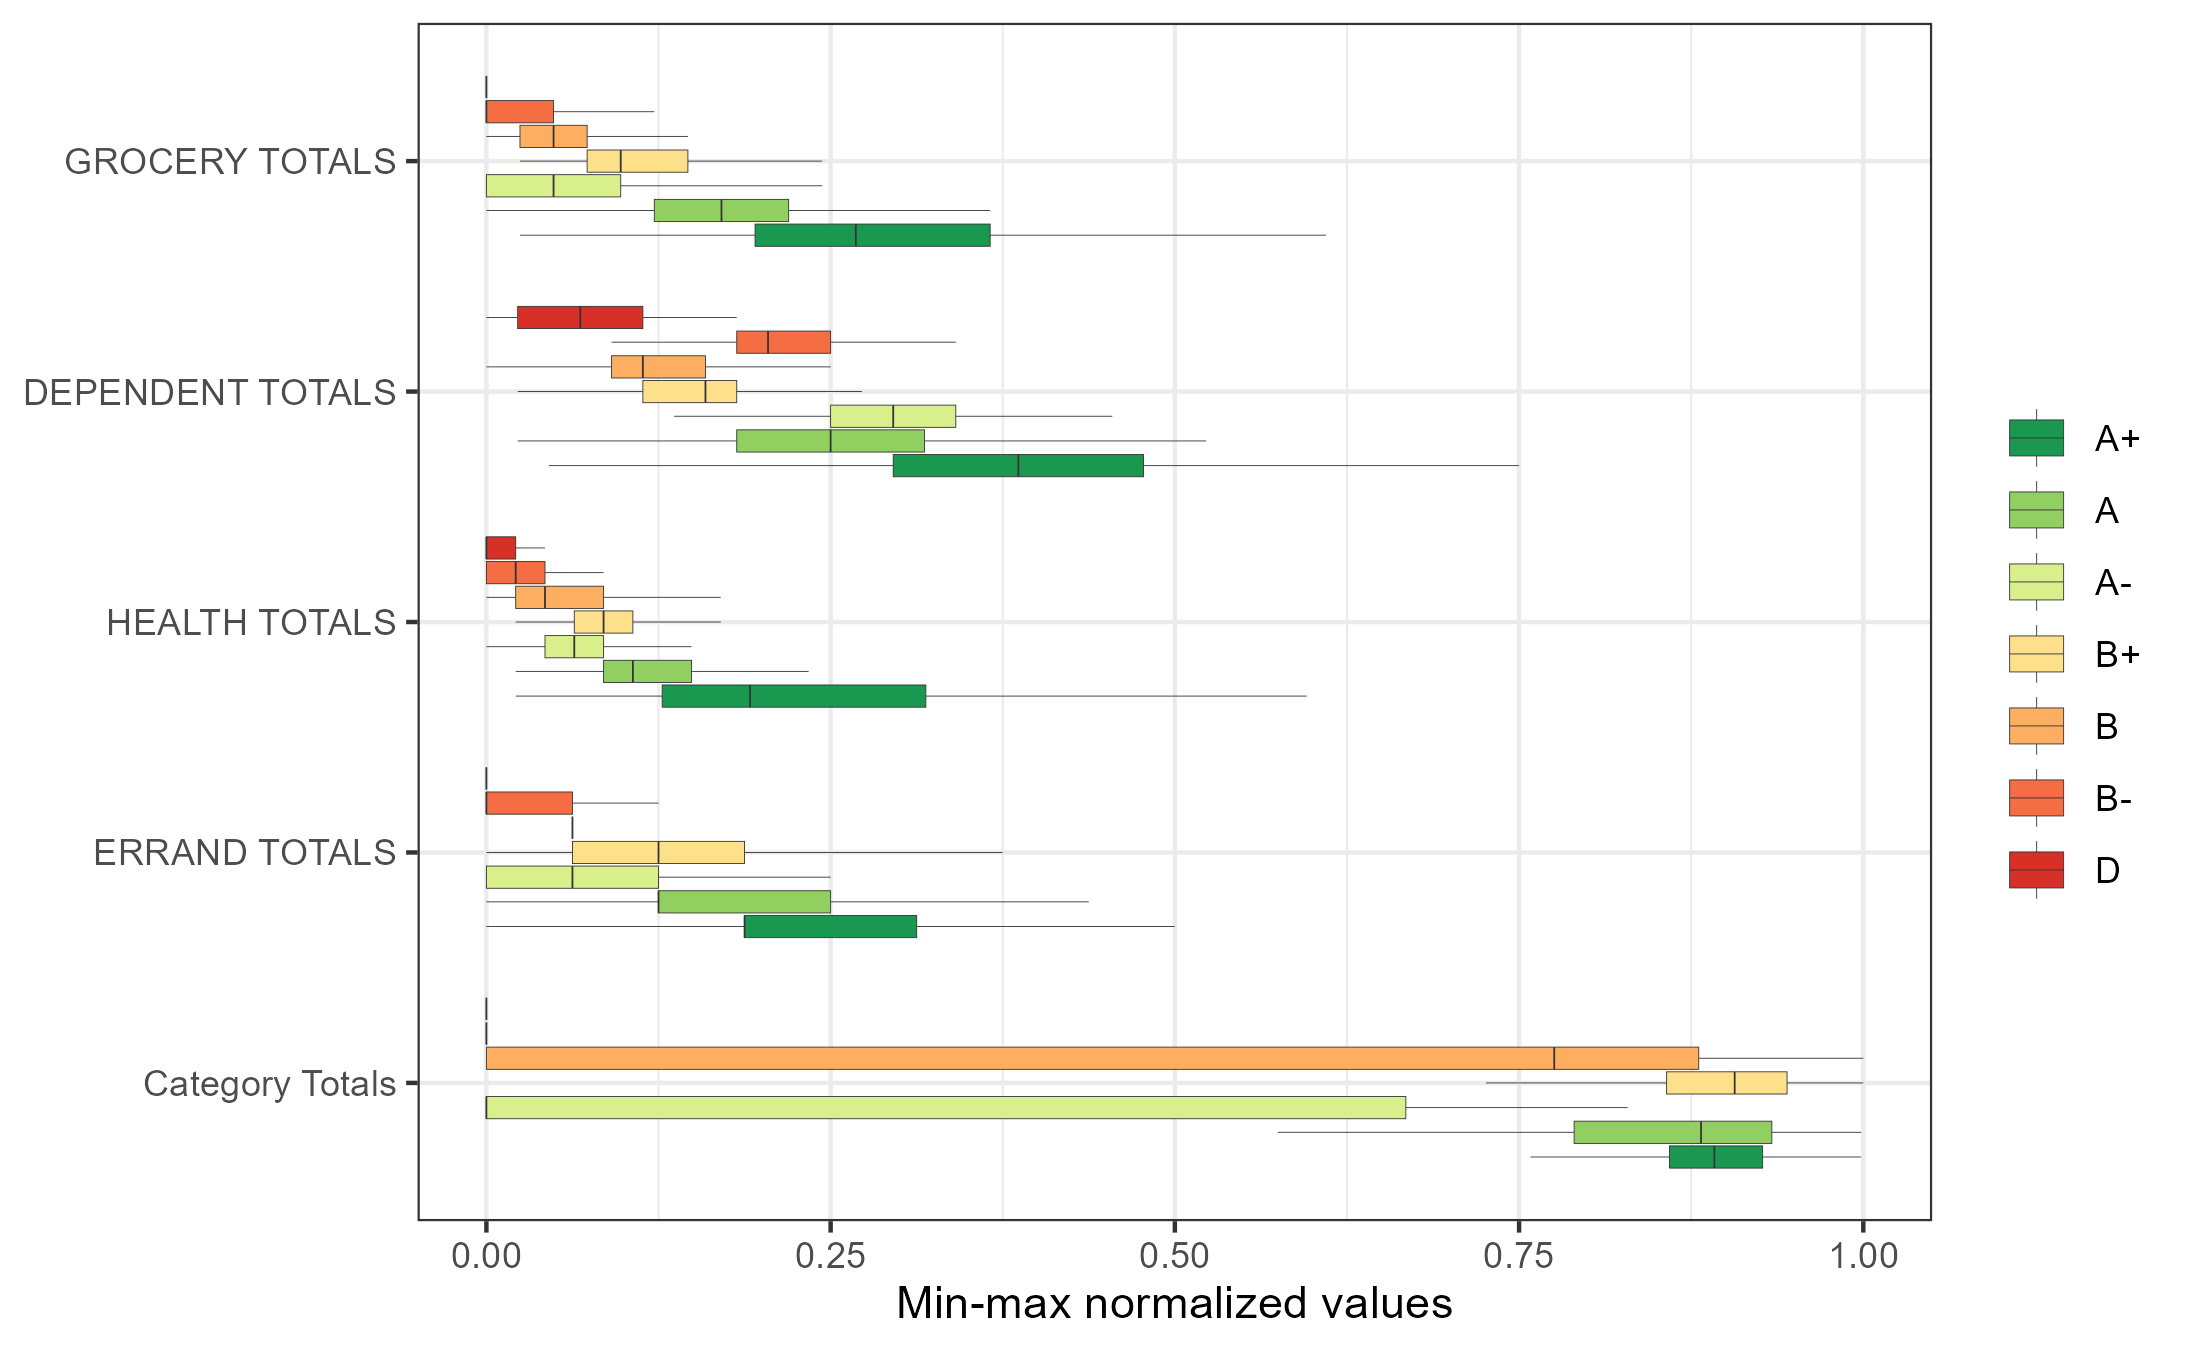
\includegraphics[width=8.33333in,height=3.125in]{../figures/box-plot.png}

}

\caption{\label{fig-Fig7}A boxplot demonstrating summary variables and
category diversity that define the superclusters.}

\end{figure}%

\newpage

To spatially demonstrate where the superclusters are located,
representative supercluster labels for each DA are visualised in
Figure~\ref{fig-Fig8}. This visualisation is created by grouping parcels
by their DA, calculating the median supercluster label for each label,
and selecting the label that is most dominant within that DA. For
reference, the median number of parcels in each DA is 150 and
supercluster label membership within a DA is typically pure, with the
median membership being 80\% of a single cluster.

\begin{figure}

\centering{

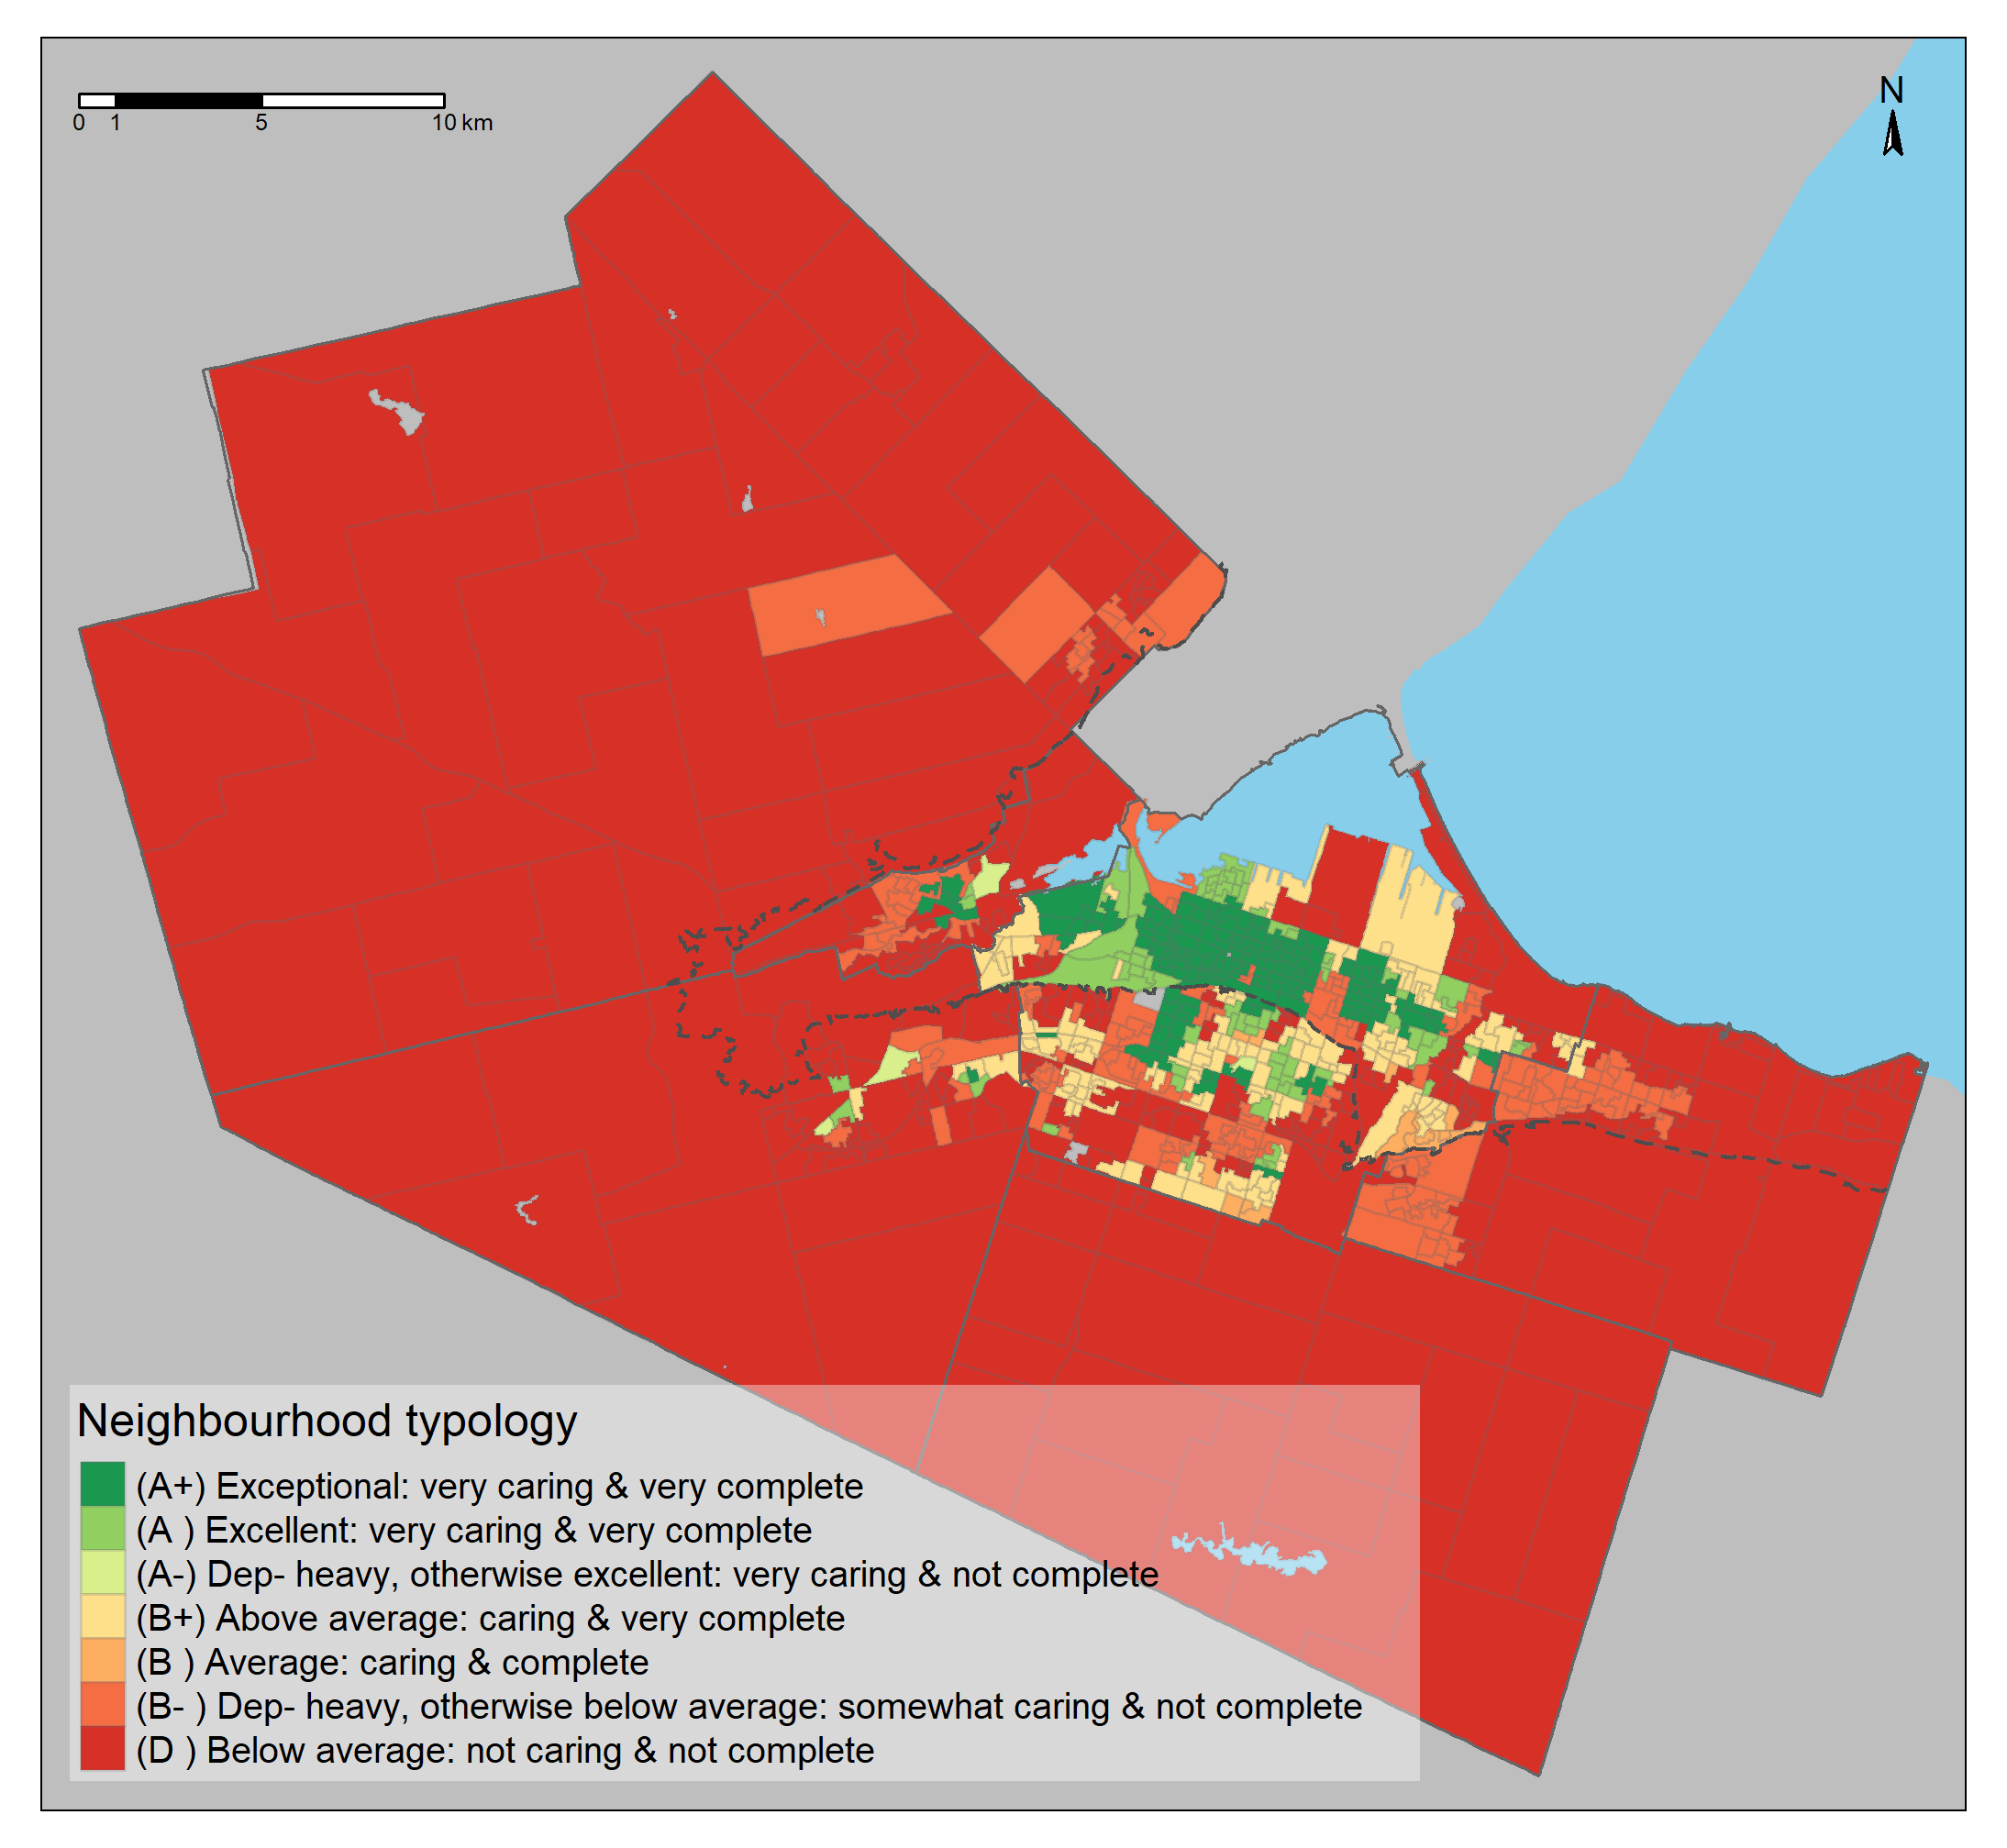
\includegraphics[width=4.6875in,height=4.6875in]{../figures/SClabel_plot.png}

}

\caption{\label{fig-Fig8}The maximum median parcel supercluster
membership per DA. Escarpment is visualised as a grey dashed line.
Basemap shapefiles are retrieved from the 2021 Canadian census
\citep{governmentofcanadaCensusPopulation2023}, the Open Data Hamilton
Portal \citep{opendatahamiltonCityBoundary2023} and the USGS
\citep{greatlakesUSGS2010}.}

\end{figure}%

The resulting superclusters visualised in Figure~\ref{fig-Fig8} are a
combination of the cumulative opportunity and diversity of access
measures translated into meaningful typologies through the SOM
methodology. To reiterate, accessibility is the measure of
\emph{potential} interaction, e.g., how many care destinations one could
reach within a 15-minute walk, these typologies are useful in
identifying which areas of the city are providing regionally high levels
of complete caring access, which areas are regionally average, and which
areas are regionally below average. Furthermore, neighbourhoods which
provide disbalanced access can be further investigated.

In Figure~\ref{fig-Fig8}, it can be observed that the excellent and
exceptional neighbourhoods (A, A+), which are very caring and very
complete 15-minute neighbourhoods, are located within the center of the
city and closest to the shoreline in the downtown core of Hamilton. The
above and below average neighbourhoods (B+ B) are often proximate to the
excellent and exceptional neighbourhoods and are more prevalent in south
of the escarpment within the center Hamilton. The escarpment is a
physical barrier, with few pedestrian-accessible access points to
traverse; hence the typologies describing neighbouring DAs separated by
the escarpment are often different. Below average (D) neighbourhoods are
located in peripheral areas outside the center of Hamilton, in areas
where urban form is characterised by lower density residential housing
and auto-dependent mobility.

Furthermore in Figure~\ref{fig-Fig8}, A- and B- grades stand out as
offering high access for children-centric destinations for their
grade-group but below grade-group average access in other destination
types. These neighbourhoods may be more suitable for populations who
prioritize walkable access to destinations like schools, parks and
daycares, and find access to other types of caring destinations less
important. These neighbourhoods also stand out as demonstrating
potential to be retrofitted to provide more complete access if
additional destination types were located within their neighbourhoods.

\subsection{Profiles of who does and does not reside in caring 15-minute
neighbourhoods}\label{profiles-of-who-does-and-does-not-reside-in-caring-15-minute-neighbourhoods}

To enhance the meaning of the superclusters beyond a descriptive and
spatial conceptualisation of ``caring'' and ``complete'', \emph{who?}
resides in what neighbourhood is investigated through the Decision Tree
results. The input features of the Decision Tree are the supercluster
labels and the feature variables are various population-weighted
socio-demographic characteristics of the 2021 Canadian Census, namely:
median household income, \% below the median household income, \% LICO
prevalence, average number of children per household, \% population aged
0 to 14, \% not in the labour force, \% not employed, Gini index on
adjusted household after-tax income, \% visible minority, \% single
parent household, \% who walk to work (relative to bike, care/truck/van,
public transit and `other'), \% of owner household in core housing need
(i.e., inadequate housing structure or paying higher than 30\% income on
housing), \% of tenant households in subsidized housing, \% of tenant
households in core housing need, \% no certification or with only a
highschool diploma.

Of all the included input variables, \emph{median household income}
proved to be the most meaningful in partitioning the superclusters data.
Figure~\ref{fig-Fig9} provides the Decision Tree with the significant
splits in median household income and the proportion composition of
supercluster along each branch for three terminal Decision Tree nodes.
While the algorithm is unable to homogenously use each supercluster,
Figure~\ref{fig-Fig9} is helpful to report a narrative of who may reside
in what caring/complete supercluster. Particularly, the Decision Tree
demonstrates a more pure supercluster membership for only two of the
three terminal Decision Tree nodes: supercluster A+ (exceptional
completely caring access) and D (not caring and complete access). For
reference, the city-wide mean household income is 81,316 (SD: 25,239 and
median: 80,000). The notable splits for income are \textgreater\$91,500,
\textgreater\$68,750, or between \$68,750 and \$91,500; roughly split by
lower income, middle income, and higher income median household
brackets.

\begin{figure}

\centering{

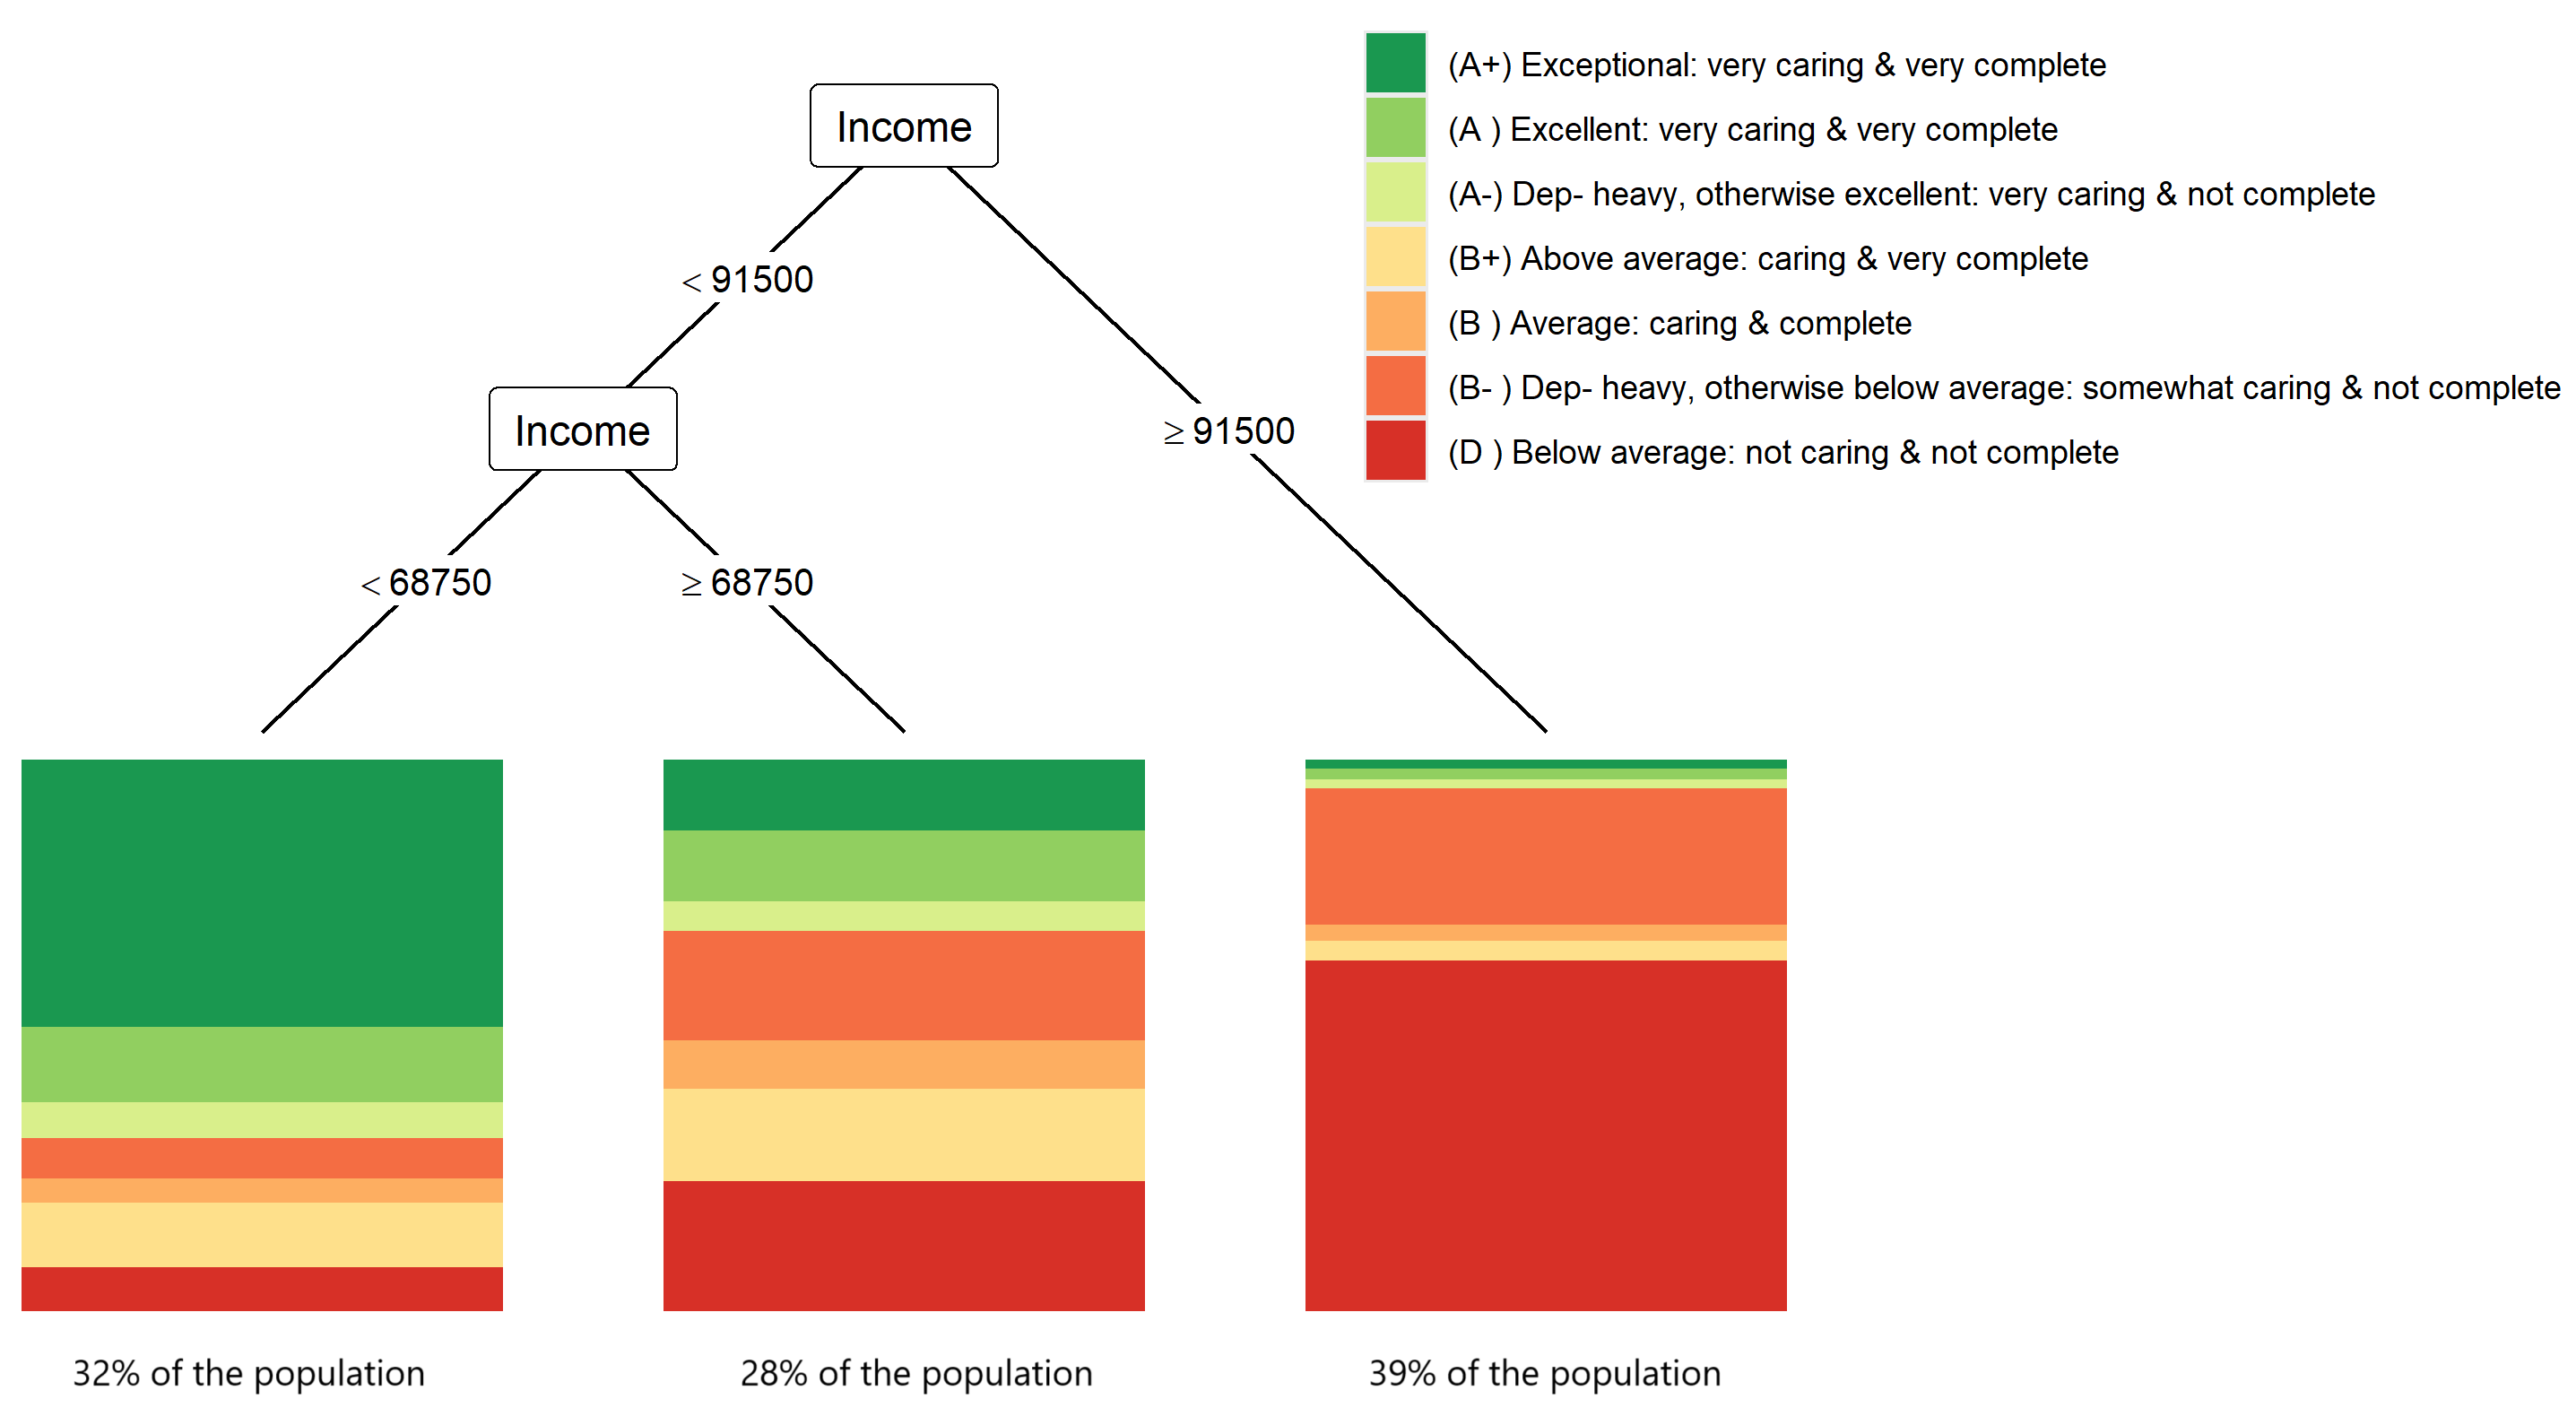
\includegraphics[width=6.25in,height=4.6875in]{../figures/access_sc_profiles_justincome.png}

}

\caption{\label{fig-Fig9}The Decision Tree demonstrating median
household income splits and superclusters composition within each
branch.}

\end{figure}%

Describing Figure~\ref{fig-Fig9}, the bar column on the right represents
DAs with higher household income. In these DAs, the majority of parcels
are labeled as D superclusters, i.e not caring or complete 15-minute
neighbourhoods. Within this higher-income-representing bar column, the
second highest proportion of supercluster membership are B- parcels. B-
parcels are low in most amenity types except a few child-centric
destinations and show promise in being more easily improved than the D
parcels. The higher income column represents 39\% of the population, the
largest proportion of any of the three columns. The left column in
Figure~\ref{fig-Fig9} corresponds to the lowest income, i.e., below
68,750 CAD median household income, and accounts for 32\% the
population. It is dominated by A+ parcels along with A and A- parcels,
in the largest quantities relative to other bar columns, however,
proportions of all other superclusters are also present. The middle
column is defined by parcels with a mix of supercluster classifications
and represents DAs with middle households incomes, between 68,750 CAD
and 91,500 CAD representing 28\% of the population.

Though median income was the most useful in partitioning the parcels by
their supercluster labels in Figure~\ref{fig-Fig9}, other variables are
still important. Namely, the following variables in order of importance
and correlation coefficient with the median household income variable in
brackets, are listed: the \% below the median household income (-0.89),
\% single parent household (-0.57), \% no certification or with only a
highschool diploma (-0.49), the average number of children per household
(0.38), \% not in the labour force (-0.41), \% LICO prevalence (-0.67),
and \% who walk to work (-0.37).

It is notable that median household income is highly or moderately
correlated with many of these important variables, and discussing these
correlations is useful for interpretation alongside the Decision Tree
diagram. For instance, single-parent families are most positively
correlated with the proportion of households being in the bottom income
distribution (-0.89) and lower or no diploma (0.6), and most negatively
with the median after-tax household income (-0.57), reflecting
nationwide trends
\citep{governmentofcanadaDailyMainHighlights2024, governmentofcanadaPrevalenceLowIncome2024}.
Though not all single-family households are below the LICO (i.e.,
single-family households are not highly correlated with LICO at the
DA-level in Hamilton), DAs with higher concentrations of single-family
households and LICO prevalence tend to have A+ access. Conversely, DAs
with lower single-parent households are in DAs with a higher
concentration of parcels with D access. These findings are notable from
an equity perspective since economic disadvantaged often intersects with
other socio-demographic characteristics.

\section{Discussion}\label{discussion}

Geographically, Hamilton is city that offers very caring - and
completely caring - 15-Minute neighbourhoods for some, but not all.
There are evident spatial inequalities, with areas ranging from
excellent (A+ and A), average (B+ and B), to well below average (D).
Some areas, like those labelled A- and B-, show potential for
improvement within their grade groups. While the downtown core has the
highest concentration of \emph{caring 15-minute neighborhoods}, certain
areas outside the core do as well. This finding somewhat contrasts
employment accessibility studies, such as
\citet{elgeneidyNonstopEquityAssessing2016}'s assessment of public
transit access to employment in the Greater Toronto Area (including
Hamilton), where access is heavily concentrated in the downtown core,
more so than appears to be present in this work. Though our paper uses a
different methodology, both studies highlight distinct patterns: indeed,
A+, A or A- care access is concentrated in the downtown core but it is
also present in certain pockets outside of the center of Hamilton,
leading to interesting conjectures. For instance, some of the A-grade
neighborhoods in Hamilton likely follow land-use principles that
emphasized residential proximity to amenities, similar to the NUC
reviewed. The potential overlap of the NUC with caring 15-minute
neighborhoods warrants further investigation.

Who currently resides in Hamilton's completely caring 15-Minute
neighbhorhoods is also demonstrated to be a somewhat optimistic story.
Parcels that provide A+ completely caring access tend to be in DAs that
are economically disadvantaged. Economic disadvantage tends to intersect
with other identities such as gender
\citep{lightmanMeasuringEconomicExclusion2018}. And as reviewed in this
work, all women and especially those from lower income households tend
to complete most Mobility of Care trips
\citep{ravensbergen2023exploratory}. Furthermore, lower-income
households tend to also be single-parent households. Broadly,
single-parent households are more likely to be time-disadvantaged
\citep{nieuwenhuisSingleparentFamiliesWork2018}, and tasked with a
higher proportion of care duties \citep{craigTimeCareComparison2004}. In
this way, the most economically disadvantaged groups having A+ complete
and caring access is an optimistic finding. However, Hamilton is
experiencing gentrification \citep{ellisyoungWeReJust2018}; rents are
rising along the future light rail transit corridor and throughout the
city
\citep{vandermerweSpilloverGentrificationMidsized2021, mayersLightTransitDocumenting2023}.
Toronto, Hamilton's larger and higher-rent neighbouring city, is
spilling gentrification into Hamilton's downtown core, (re)producing
neighbourhoods based on Toronto's middle class identities
\citep{mayersLightTransitDocumenting2023}. In these ways, the lower
income residents of Hamilton's A+ neighbourhoods are more likely to be
displaced, which is matter of wellbeing and justice. There are now few
low-rent choices that provide the same exceptional level of access as
the downtown core, hence lower household income residents that currently
reside in A+ neighhourhoods will likely displaced in the coming years if
current trends continue.

In discussing policy interventions that equitably increase completely
caring 15-Minute neighbourhoods in Hamilton, this work's presents a
methodology to create city-wide relative typologies and investigate who
currently resides in what neighbourhood, as a stepping stone for further
investigation. Neighbourhoods with the lowest grades (D) and with the
highest potential in being improved (i.e., high accessibiltiy for
certain types of destinations but not all) are neighbourhoods with B-
and A- grades. However, the work's findings demonstrate a mismatch in
household income and completely caring access: higher income areas are
often the ones targeted for improvement. This raises important questions
from the land-use policy perspective that need to be further analysed.
For instance, is it equitable to focus policy on ameliorating
neighbourhoods that are already higher-rent though they tend to be more
rural, single-use zoned and car-dependent (parcels with D grades)?
Further, of the parcels that provide high child-centrics but low
otherwise, A- parcels (better access) tend to be in DAs with
lower-income households more so than B- parcels (lower access than A-).
From the perspective of ameliorating land-use to support the equitable
distribution of 15-minute caring neighbourhoods which areas be targeted?
Who should benefit, and how? If the policy initiative is targeted to
specific neighbourhoods: sustainability linked to car dependency and
equity are in tension. This harkens to what role a planned
neighbourhood, and bottom-up planning approaches that include the
evaluation of travel behaviour by socio-economic and demographic profile
should be adopted to achieve equitable 15-minute cities.

As is the case for all research, the results should also be interpreted
along with methodological assumptions. This work measures spatial
accessibility which is a measure of potential interaction with all
reachable destinations from an origin. These destinations, however, may
not be relevant to people at an origin, e.g., they may be underutilized
(walkable access to 2 schools may be underused, as children often only
attend 1 school), the trip physically undesirable (the walk may be along
an arterial with high traffic speeds, making the trip unlikely to ever
happen by foot), or the average walking speed assumed may not reflect
the walking speeds of all populations
\citep{willberg15minuteCityAll2023}. Further, people who reside in these
neighbourhoods may also disagree with the neighbourhood's label. The
grade labels are region-relative (e.g., high accessibility in Hamilton
may be subjectively insufficient for some) and they do not consider
subjective perceptions that influence accessibility (e.g., though a
neighbourhood has many opportunities, it may not feel safe to access
them). Furthermore, accessibility is calculated from the point of
residential parcels. Care trips are not necessarily completed from home,
in-fact, they are often completed in complex trip-chains
\citep{scheinerWomenComplexDaily2015}. In this way, the results flatten
the dynamic patterns of care trips. These methodological assumptions
should all be taken together when interpreting the results. In this way,
the methodologyand findings presented identifies spatial and
socio-economic trends that should be further investigated.

\section{Conclusion}\label{conclusion}

This study makes three types of contributions to the transportation and
city planning literature: empirical, methodological and theoretical. At
the empirical level, areas of the mid-sized City of Hamilton have been
typified by their degree of `15-Minute Caring Neighbourhood' potential.
Methodologically, we applied the longstanding accessibility measure of
cumulative opportunities and entropy to classify spatial areas based on
how many destinations could be reached in a 15-minute walk and the
diversity of destination type. These values were then clustered using a
novel machine learning approach, SOM, to generate meaningful typologies
for discussion and further comparison with socio-economic composition of
the area. We find A+ and A 15-minute caring neighbourhoods are located
within the downtown core and in certain suburban pockets of the city,
while the peripheral regions provide D level caring access. A- and B-
areas are also identified as neighbourhoods that already support a high
amount of children-centric destination access, and could be improved to
provide better complete care access. Theoretically, our work puts forth
an explicitly caring 15-Minute Neighbourhod conceptualisation, bridging
the Mobility of Care and the 15-Minute City concepts. We discuss how
measuring caring neighbourhoods can be explicitly considered within city
planning.

Our work is of relevance to researchers and practitioners planning
equitable and sustainable cities. Instead of prescribing an urban form
design principle, such as ``all local amenities should be within a
15-minute walking distance'', it instead examines an empirical example
to determine which areas in the city have the \emph{potential} to be
15-minute neighbourhood based on the existing spatial accessibility
offered by the urban environment and walking transport network. To this
end, this data-driven methodology introduces a way to identify
neighbourhoods that have potential, almost have potential, and are far
from containing this potential to support future context-specific
qualitative work.

\section{References}\label{references}

\renewcommand{\bibsection}{}
\bibliography{bibliography.bib}




\end{document}
